\documentclass{beamer}
\usetheme{Madrid}
\usecolortheme{default}
\usepackage{amsmath,amssymb,lmodern}
\usepackage[thicklines]{cancel}
\usepackage{caption}
\usepackage{listings}
\usepackage{animate}
\usepackage{subcaption}
\usepackage{xcolor}
\usepackage{graphicx} %Loading the package

\graphicspath{{figures/}} %Setting the graphicspath
\title[Machine Learning]
{Treinamento de Machine Learning e Deep Learning}

\subtitle{Do Básico ao Avançado}

\author[Mafalda, Salomão] % (optional, for multiple authors)
{Salomão Machado Mafalda\inst{1}}

\institute[PAVIC] % (optional)
{
  \inst{1}%
  Universidade Federal do Acre\\
  PAVIC

}

\date[2023] % (optional)
{2023}

\logo{
\includegraphics[height=0.8cm]{ente}}

\definecolor{uoftblue}{RGB}{6,41,88}
\setbeamercolor{titlelike}{bg=uoftblue}
\setbeamerfont{title}{series=\bfseries}

\begin{document}

\frame{\titlepage}

\begin{frame}
\frametitle{Agenda}
\tableofcontents
\end{frame}



%==========================================================================================
\section{Pytorch Workflow}

\begin{frame}
	\frametitle{Pytorch Workflow}
	\begin{block}{Pytorch Workflow}
		Agora vamos fazer tudo o que fizemos anteriormente no pytorch! \\
		Os passos básicos que sempre faremos daqui pra frente serão: 
		\begin{itemize}
			\item Escolher e Adquirir os dados
			\item Pytorch:
			\begin{itemize}
				\item Escolher modelo pre-treinado ou construir um modelo
				\item Escolher função de custo e otimizador
				\item Construir laço de treinamento
			\end{itemize}
			\item Treinar o modelo e fazer predições
			\item Avaliar o modelo
			\item Melhorar o modelo
			\item Salvar e Recarregar o modelo
		\end{itemize}
	\end{block}
\end{frame}
%==========================================================================================
\begin{frame}
	\frametitle{Pytorch Workflow}
	\begin{block}{Pytorch Workflow}
		Normalmente, os dados usados em Machine Learning são obtidos a partir de: Tabelas de Excel, Imagens de alguma coisa, Vídeos, Áudios, DNA, Texto, Etc.
	Machine Learning funciona em duas partes: \\
	1. Adquirir os dados em uma representação numérica. \\
	2. Construir um modelo capaz de aprender padrões na representação numérica.
	\begin{figure}
		\centering
		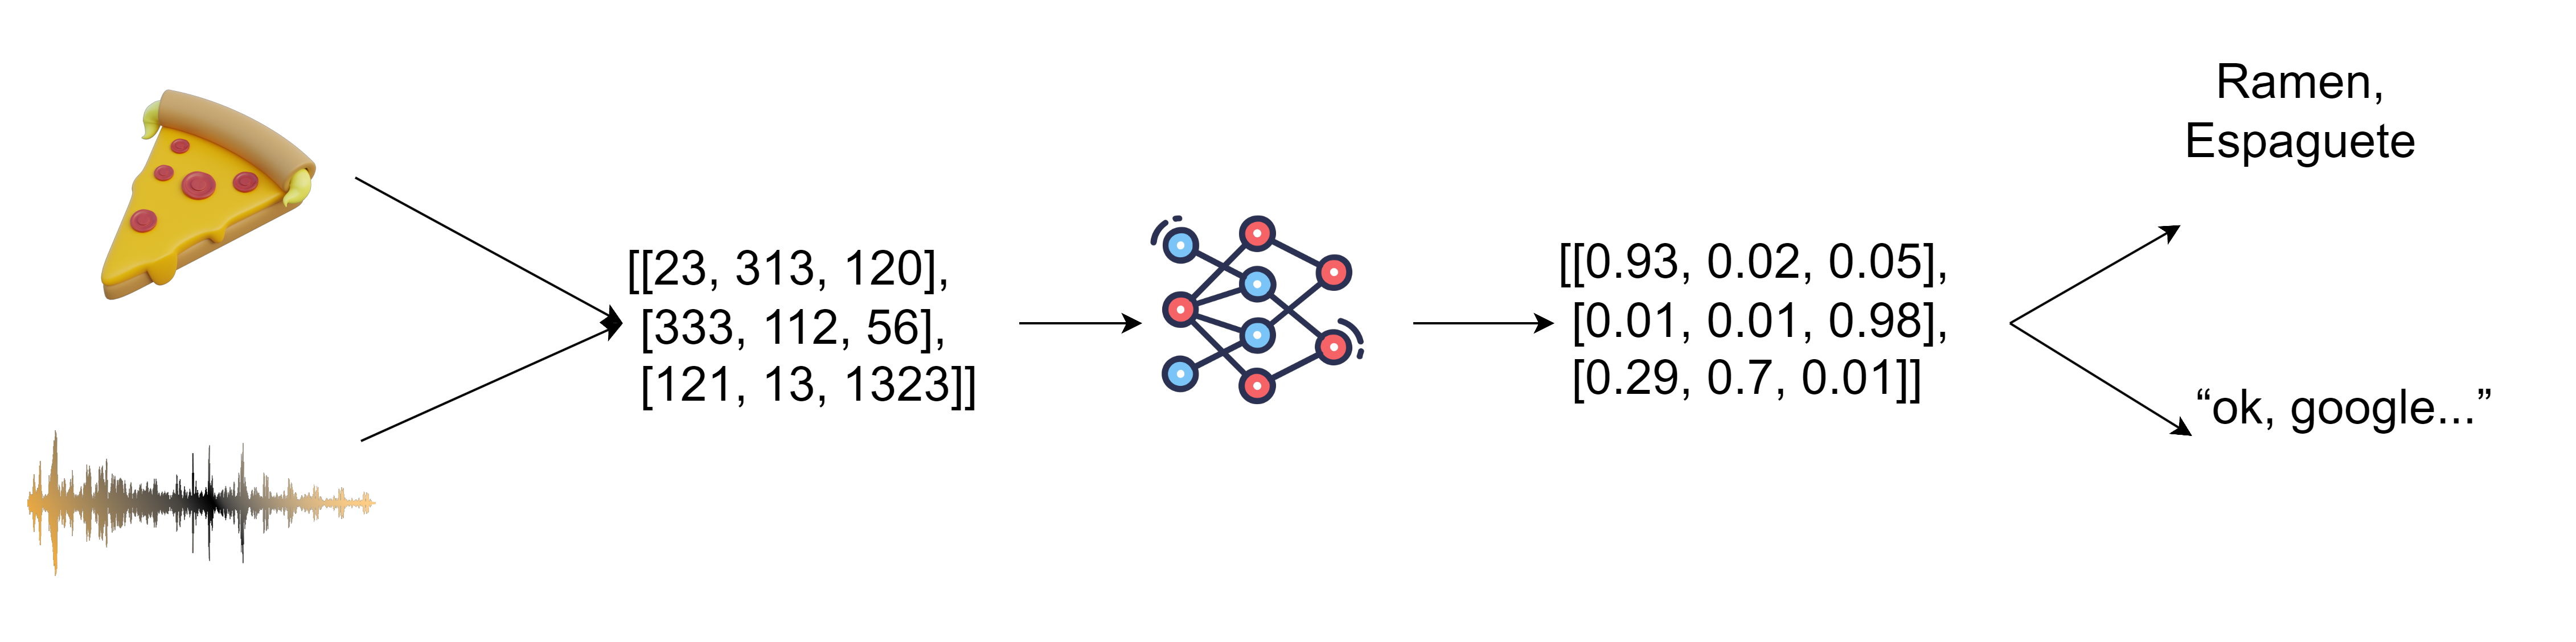
\includegraphics[width=1\linewidth]{figures/workflow_nn}
	\end{figure}
	
	\end{block}
\end{frame}

%==========================================================================================
\section{Pytorch Regressão Linear}

\begin{frame}
	\frametitle{Pytorch Regressão Linear}
	\begin{block}{Pytorch Regressão Linear}
		
		Se recordam da fórmula da função linear? 
		$$y = a + b*X$$
		
		Vamos ver isso diretamente no notebook enquanto acompanhamos os slides! \\
		Agora vamos avançar para a construção de um modelo que pode aprender a relação entre X (features) e y (labels).
	\end{block}
\begin{alertblock}{Nota}
	Vamos usar o notebook 08
\end{alertblock}
\end{frame}
%==========================================================================================

\begin{frame}
	\frametitle{Pytorch Regressão Linear}
	\begin{block}{Divida os dados em conjuntos de treinamento e teste}
		Temos alguns dados. 
		
		Mas antes de construirmos um modelo, precisamos dividi-lo. 
		
		Uma das etapas mais importantes em um projeto de aprendizado de máquina é criar um conjunto de treinamento e teste (e, quando necessário, um conjunto de validação). 
		
		Cada divisão do conjunto de dados serve a um propósito específico:
		\begin{table}[]
			\resizebox{\textwidth}{!}{%
				\begin{tabular}{|l|l|l|l|}
					\hline
					Divisão &
					Objetivo &
					Qtd. de dados &
					Frequência \\ \hline
					Treinamento &
					\begin{tabular}[c]{@{}l@{}}O modelo aprende com esses dados\\ (como os materiais do curso que você estuda durante o semestre).\end{tabular} &
					$\sim$60-80\% &
					Sempre \\ \hline
					Validação &
					\begin{tabular}[c]{@{}l@{}}O modelo é ajustado nesses dados\\ (como o exame simulado que você faz antes do exame final).\end{tabular} &
					$\sim$10-20\% &
					\begin{tabular}[c]{@{}l@{}}Muitas vezes\\ mas nem sempre\end{tabular} \\ \hline
					Teste &
					\begin{tabular}[c]{@{}l@{}}O modelo é avaliado com base nesses dados para testar o que aprendeu\\ (como o exame final que você faz no final do semestre)\end{tabular} &
					$\sim$10-20\% &
					Sempre \\ \hline
				\end{tabular}%
			}
		\end{table}
		Por enquanto, usaremos apenas um conjunto de treinamento e teste, o que significa que teremos um conjunto de dados para nosso modelo aprender e também ser avaliado.
	\end{block}
\end{frame}
%==========================================================================================
\begin{frame}
	\frametitle{Pytorch Regressão Linear}
	\begin{block}{Divida os dados em conjuntos de treinamento e teste}
		
		Podemos criá-los dividindo nossos tensores $X$ e $y$.
		
		\textbf{Observação:} Ao lidar com dados do mundo real, esta etapa normalmente é realizada logo no início de um projeto (o conjunto de teste sempre deve ser mantido separado de todos os outros dados). Queremos que nosso modelo aprenda com os dados de treinamento e depois os avalie com os dados de teste para obter uma indicação de quão bem ele \textbf{generaliza} para exemplos não vistos.
		
		O modelo que criamos vai tentar aprender a relação entre X\_train e y\_train e então avaliaremos o que ele aprende em X\_test e y\_test.
		
		Mas agora nossos dados são apenas números em uma página.
		
		Vamos criar uma função para visualizá-lo.
	\end{block}
\end{frame}
%==========================================================================================

\begin{frame}
	\frametitle{Pytorch Regressão Linear}
	\begin{block}{Vizualize, vizualize, vizualize!}
		Observação: agora é um bom momento para apresentar a você o lema do explorador de dados... "visualize, visualize, visualize!"
		
		Pense nisso sempre que estiver trabalhando com dados e transformando-os em números, se você pode visualizar algo, pode fazer maravilhas para a compreensão.
		
		As máquinas adoram números e nós, humanos, também gostamos de números, mas também gostamos de olhar para as coisas.
	\end{block}
\end{frame}
%==========================================================================================
\begin{frame}
	\frametitle{Pytorch Regressão Linear - Construção do Modelo}
	\begin{block}{Fundamentos da construção de modelos PyTorch}
		PyTorch tem quatro (mais ou menos) módulos essenciais que você pode usar para criar quase qualquer tipo de rede neural que você possa imaginar.
		
		Eles são torch.nn, torch.optim, torch.utils.data.Dataset e torch.utils.data.DataLoader. Por enquanto, vamos nos concentrar nos dois primeiros e chegar aos outros dois mais tarde (embora você possa adivinhar o que eles fazem).
		
		% Please add the following required packages to your document preamble:
		% \usepackage{graphicx}
		\begin{table}[]
			\resizebox{\textwidth}{!}{%
				\begin{tabular}{|l|l|}
					\hline
					\textbf{Módulo PyTorch} &
					\textbf{Objetivo} \\ \hline
					torch.nn &
					\begin{tabular}[c]{@{}l@{}}Contém todos os blocos de construção para gráficos computacionais\\ (essencialmente uma série de cálculos executados de uma maneira particular).\end{tabular} \\ \hline
					torch.nn.Parameter &
					\begin{tabular}[c]{@{}l@{}}Armazena tensores que podem ser usados com nn.Module. Se os gradientes requires\_grad=True\\ (usados para atualizar os parâmetros do modelo por meio de gradient descent) forem calculados automaticamente,\\ isso é muitas vezes referido como "autogrado".\end{tabular} \\ \hline
					torch.nn.Module &
					\begin{tabular}[c]{@{}l@{}}A classe base para todos os módulos de rede neural, todos os blocos de construção para redes neurais são subclasses.\\ Se você estiver construindo uma rede neural no PyTorch, seus modelos devem subclassificar nn.Module.\\ Requer que um método forward() seja implementado.\end{tabular} \\ \hline
					torch.optim &
					\begin{tabular}[c]{@{}l@{}}Contém vários algoritmos de otimização (estes dizem aos parâmetros do modelo armazenados em\\ nn.Parameter como alterar melhor para melhorar a descida do gradiente e, por sua vez, reduzir a perda).\end{tabular} \\ \hline
					def forward() &
					\begin{tabular}[c]{@{}l@{}}Todas as subclasses nn.Module requerem um método forward(), que define a computação que ocorrerá\\ nos dados passados para o nn.Module específico (por exemplo, a fórmula de regressão linear acima).\end{tabular} \\ \hline
				\end{tabular}%
			}
		\end{table}
	\end{block}
\end{frame}
%==========================================================================================
\begin{frame}
	\frametitle{Pytorch Regressão Linear - Construção do Modelo}
	\begin{block}{Fundamentos da construção de modelos PyTorch}
		\begin{figure}
			\centering
			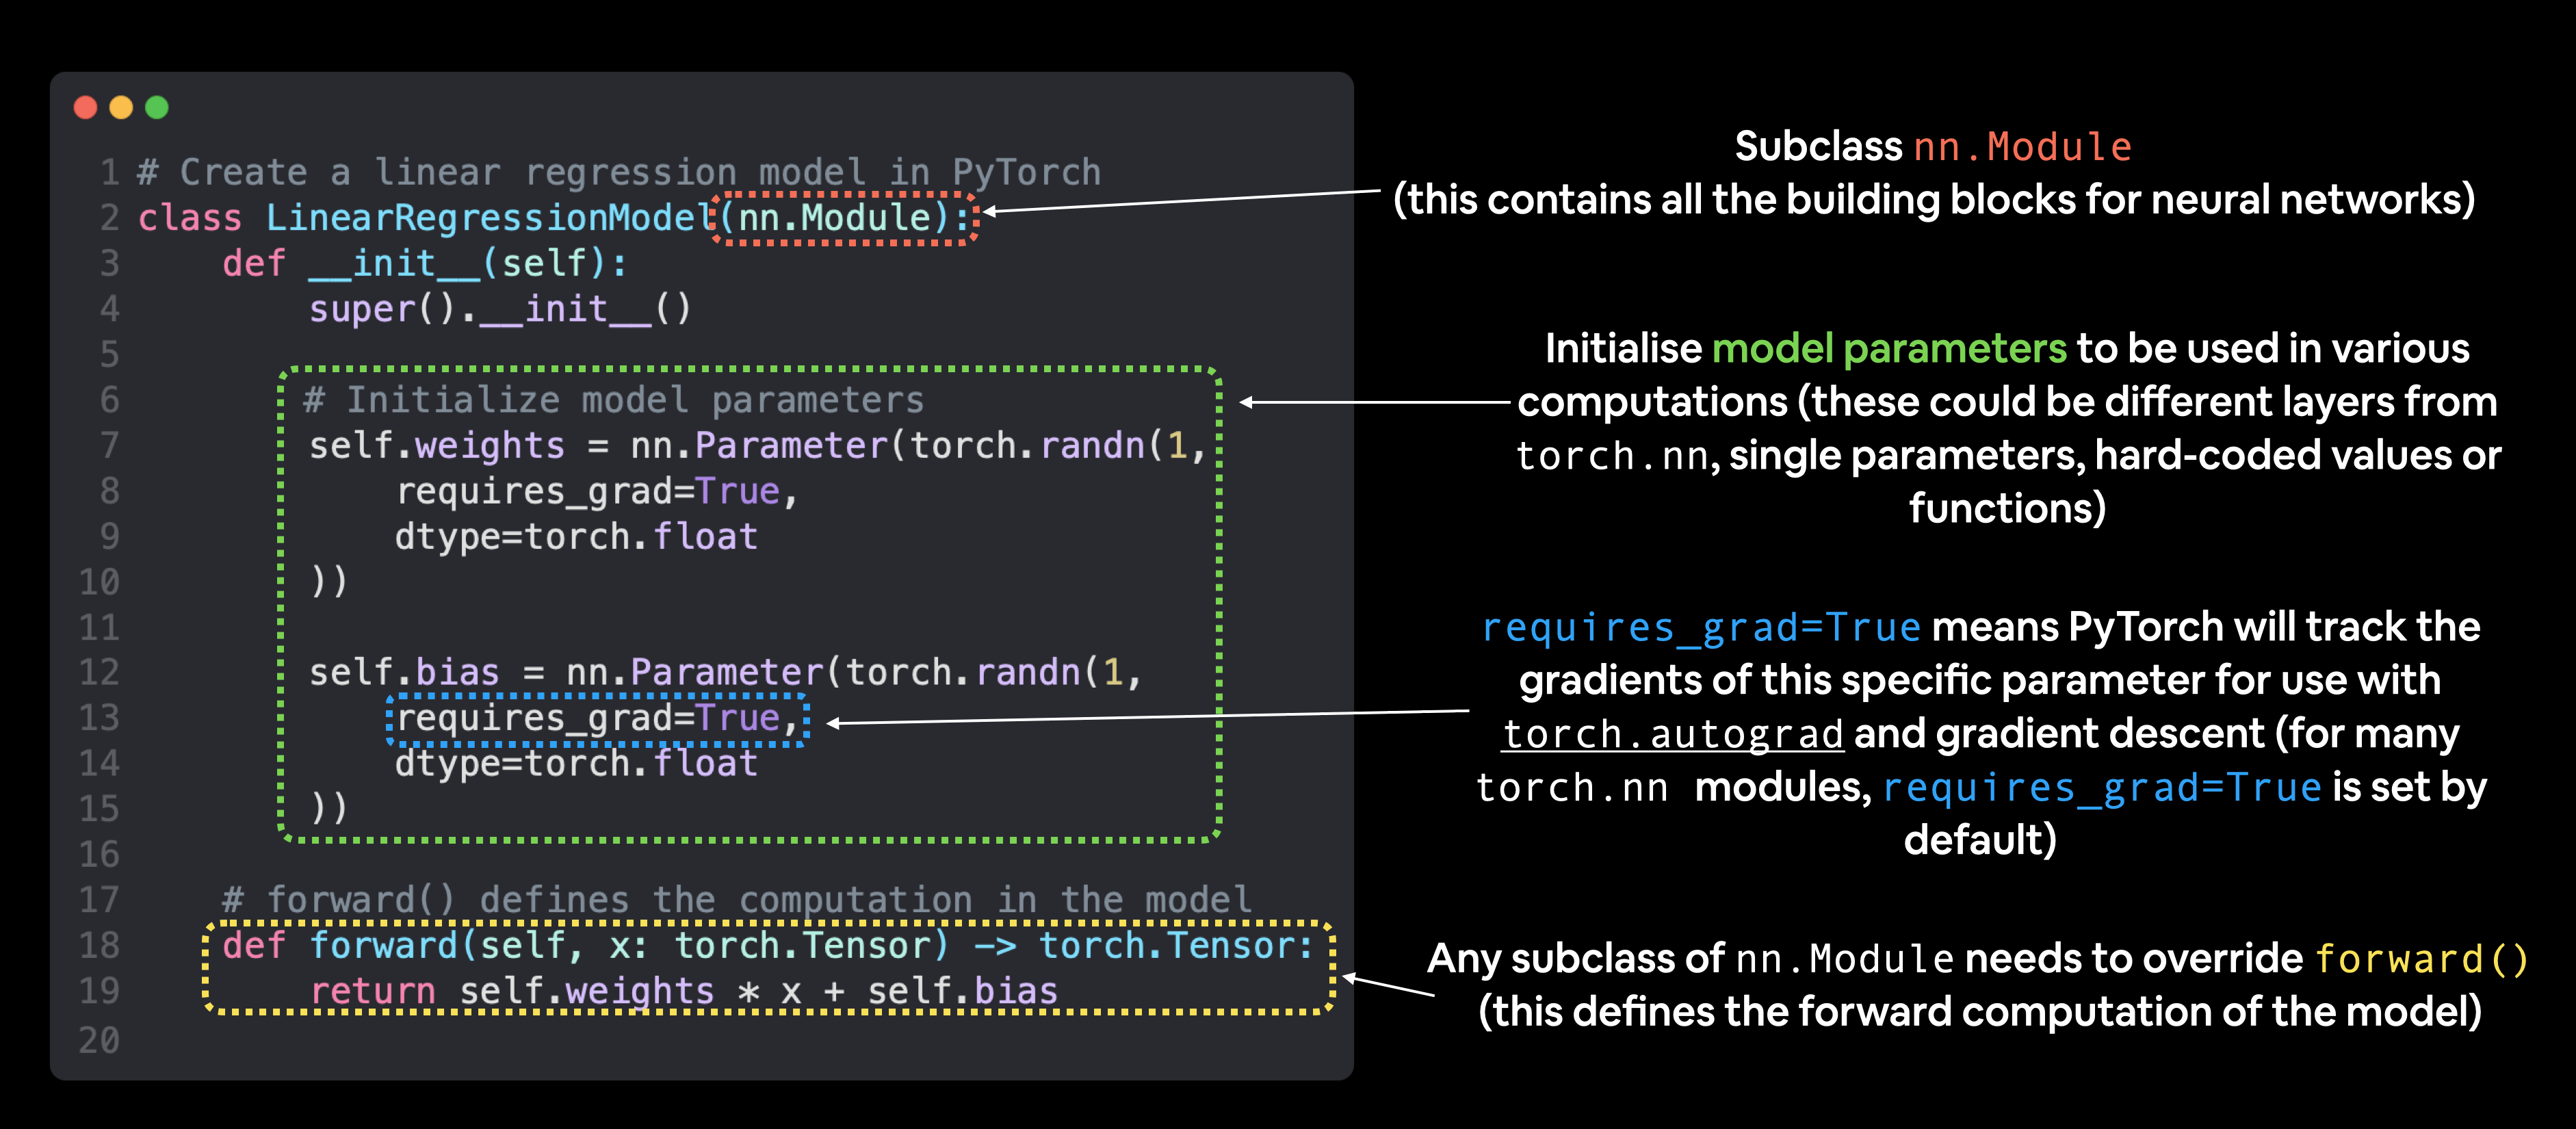
\includegraphics[width=1\linewidth]{figures/basic_torch_implmentation}
		\end{figure}
		
	\end{block}
\end{frame}
%==========================================================================================
\begin{frame}
	\frametitle{Pytorch Regressão Linear - Fazendo predições}
	\begin{block}{Fazendo predições sem treinar o modelo}
		\begin{figure}
			\centering
			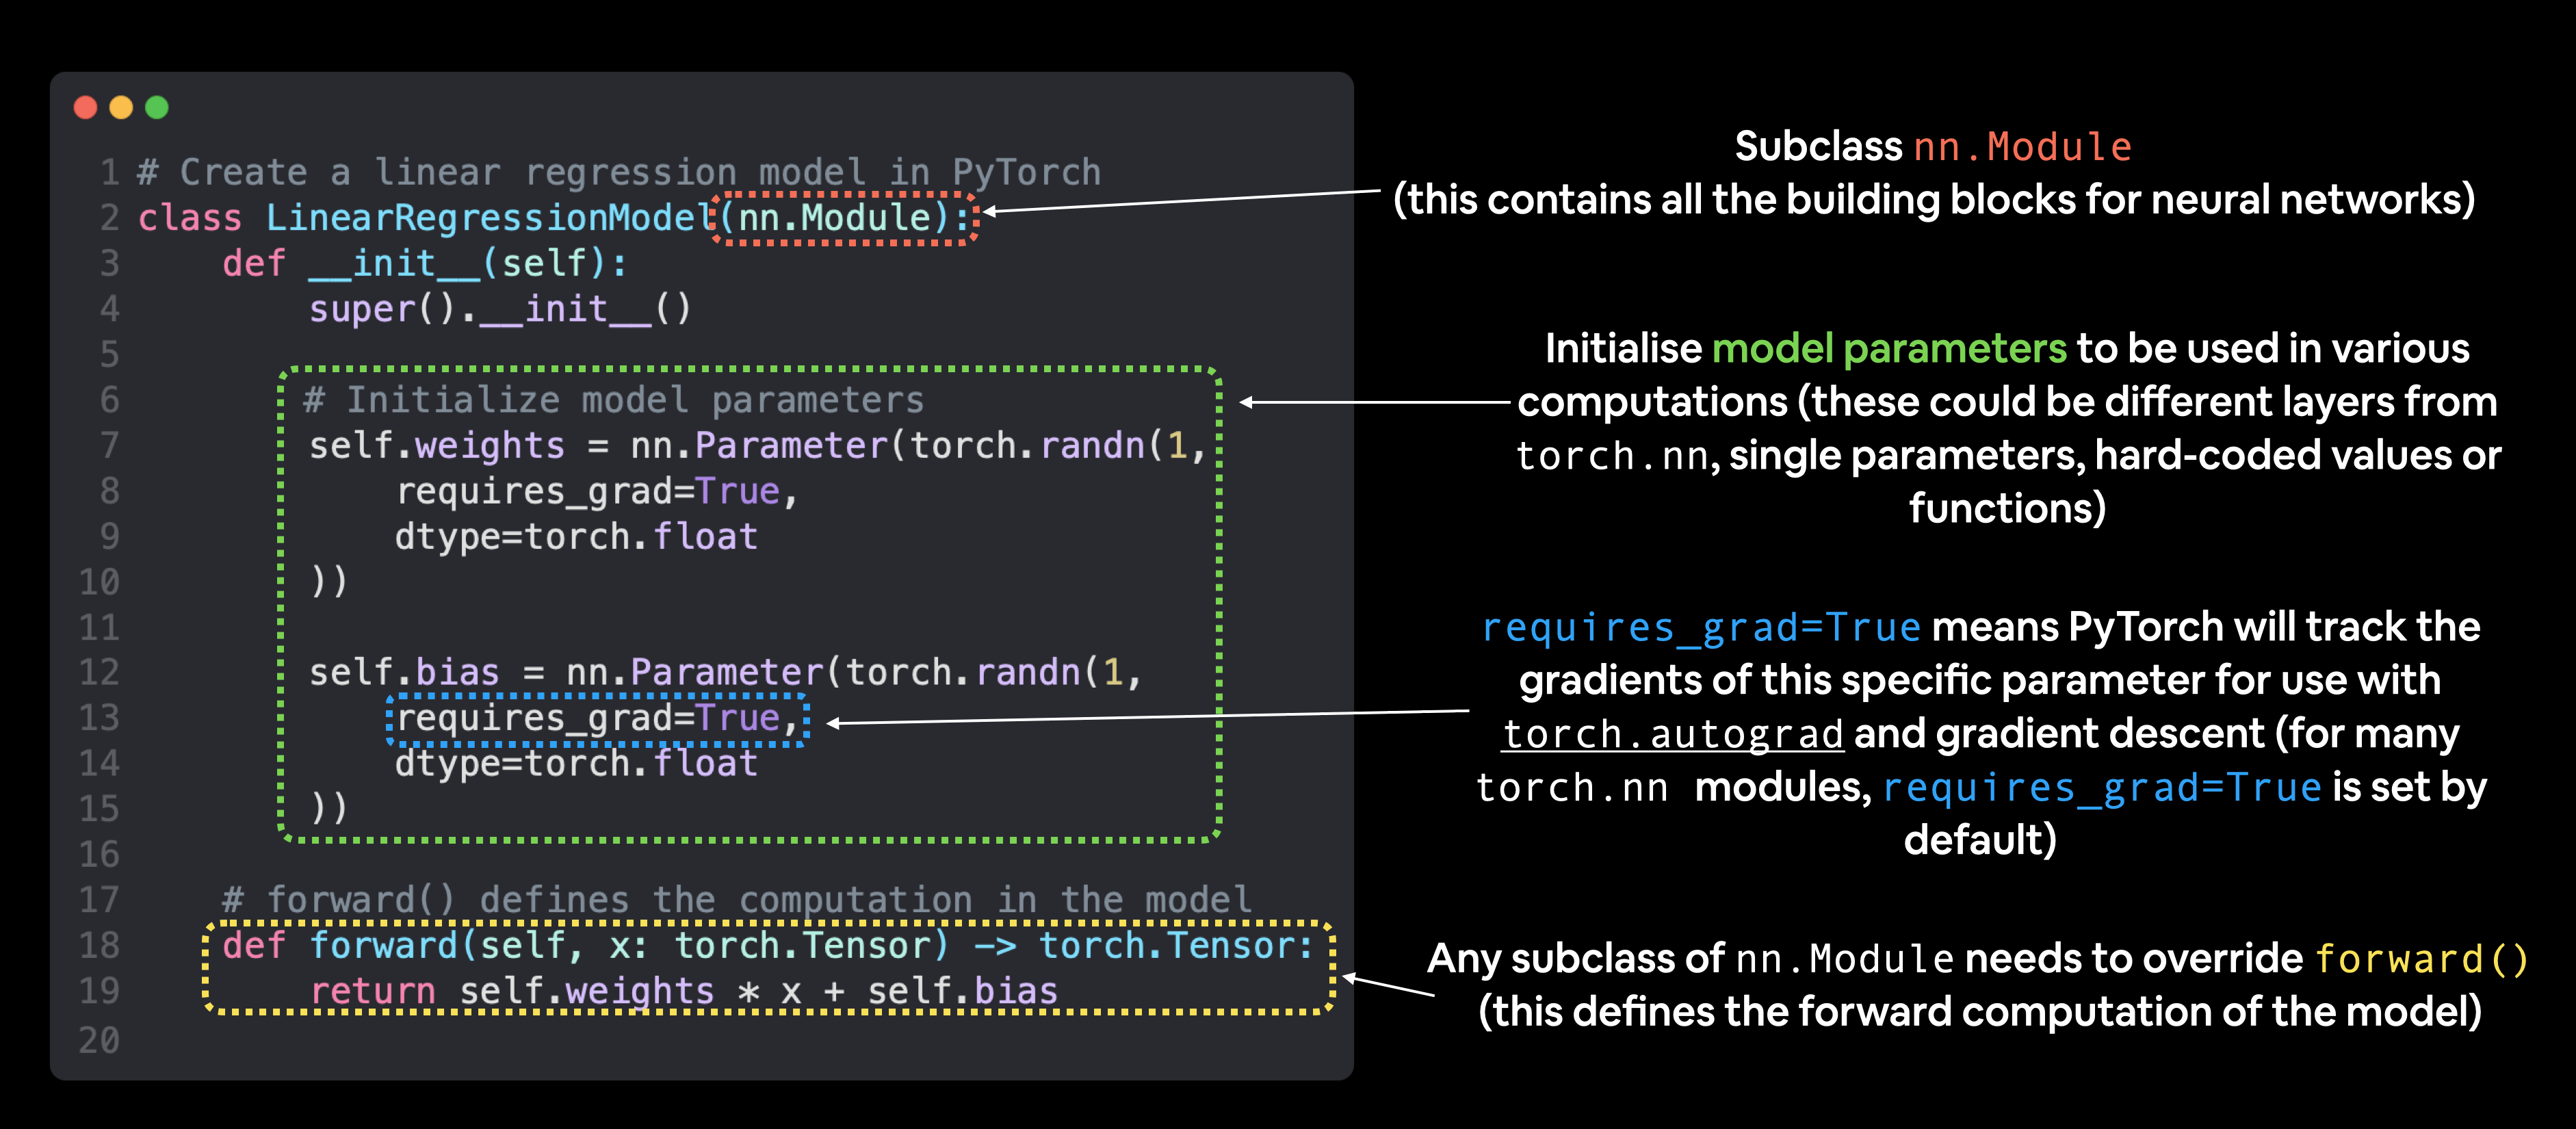
\includegraphics[width=1\linewidth]{figures/basic_torch_implmentation}
		\end{figure}
		
	\end{block}
\end{frame}
%==========================================================================================
\begin{frame}
	\frametitle{Pytorch Regressão Linear - Treinando o Modelo}
	\begin{block}{Treinando o modelo}
		\begin{itemize}
			\item Selecione a função de perda:
			\begin{itemize}
				\item Mean absolute error (MAE) for regression problems (torch.nn.L1Loss())
				\item Binary cross entropy for binary classification problems (torch.nn.BCELoss()).
			\end{itemize}
			\item Selecione seu otimizador:
				\begin{itemize}
					\item Stochastic gradient descent (torch.optim.SGD()).
					\item Adam optimizer (torch.optim.Adam()).
				\end{itemize}
			\item Crie seu loop de teinamento!
		\end{itemize}
		
	\end{block}
\end{frame}
%==========================================================================================
\begin{frame}
	\frametitle{Pytorch Regressão Linear - Treinando o Modelo}
	\begin{block}{Criando o loop de treinamento do modelo para o \textbf{Treinamento}}
		\begin{itemize}
			\item[1] Forward pass $model(x_train)$ 
			\item[2] Calcule a perda $loss = loss_fn(y_pred, y_train)$
			\item[3] Gradientes zero $optimizer.zero_grad()$
			\item[4] Executar retropropagação na perda $loss.backward()$
			\item[5] Atualize o otimizador (descida de gradiente) $optimizer.step()$
		\end{itemize}
		\begin{figure}
			\centering
			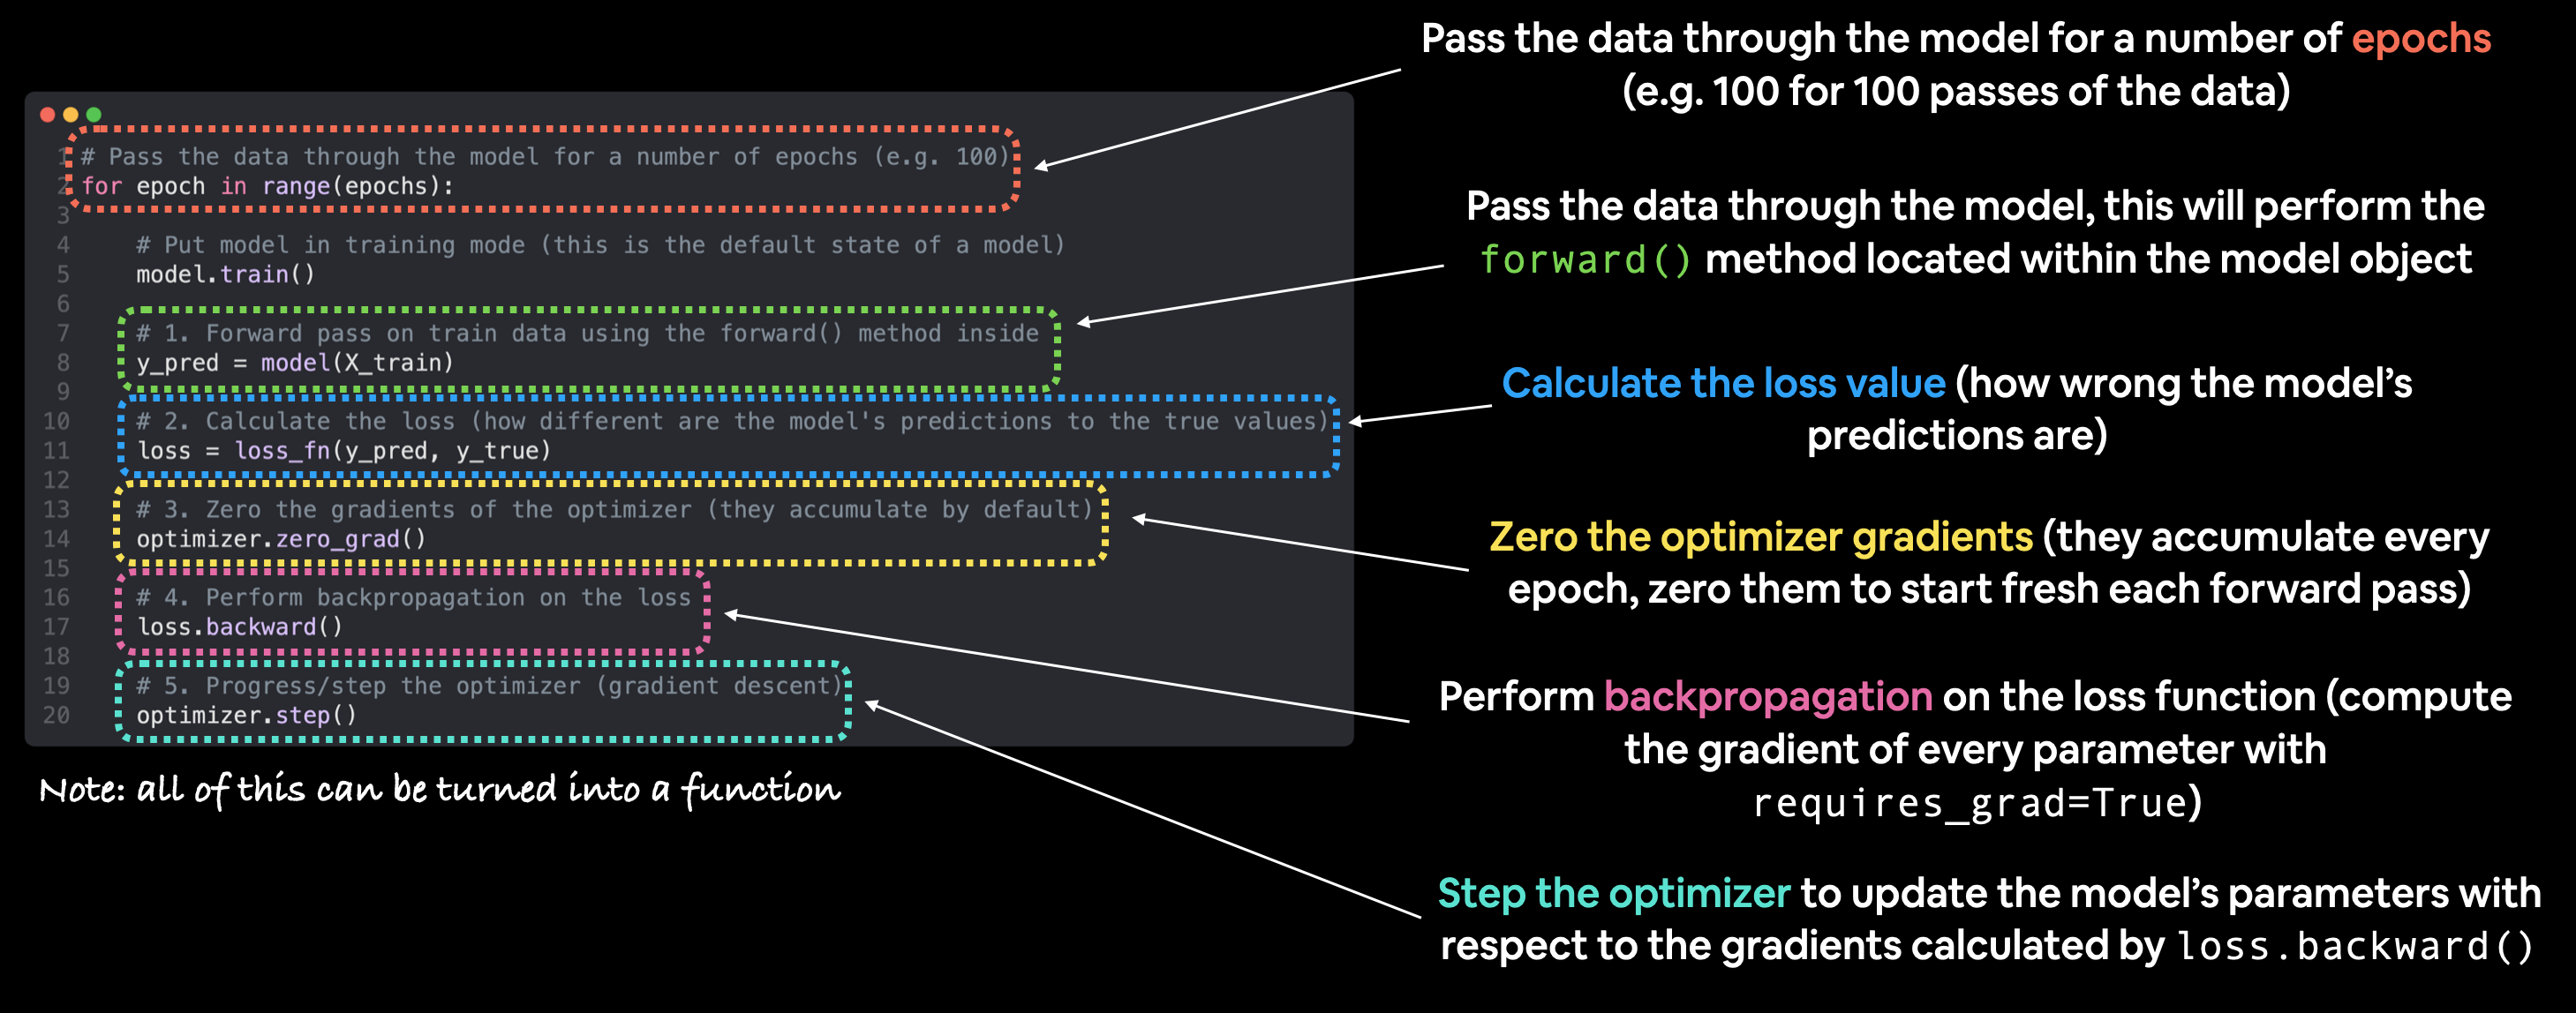
\includegraphics[width=0.7\linewidth]{figures/steps_train_torch}
		\end{figure}
		
	\end{block}
\end{frame}
%==========================================================================================

\begin{frame}
	\frametitle{Pytorch Regressão Linear - Treinando o Modelo}
	\begin{block}{Criando o loop de treinamento do modelo para o \textbf{Teste}}
		\begin{itemize}
			\item[1] Forward pass $model(x_train)$ 
			\item[2] Calcule a perda $loss = loss_fn(y_pred, y_train)$
			\item[3] Calulate evaluation metrics (optional) $Custom functions$
		\end{itemize}
		\begin{figure}
			\centering
			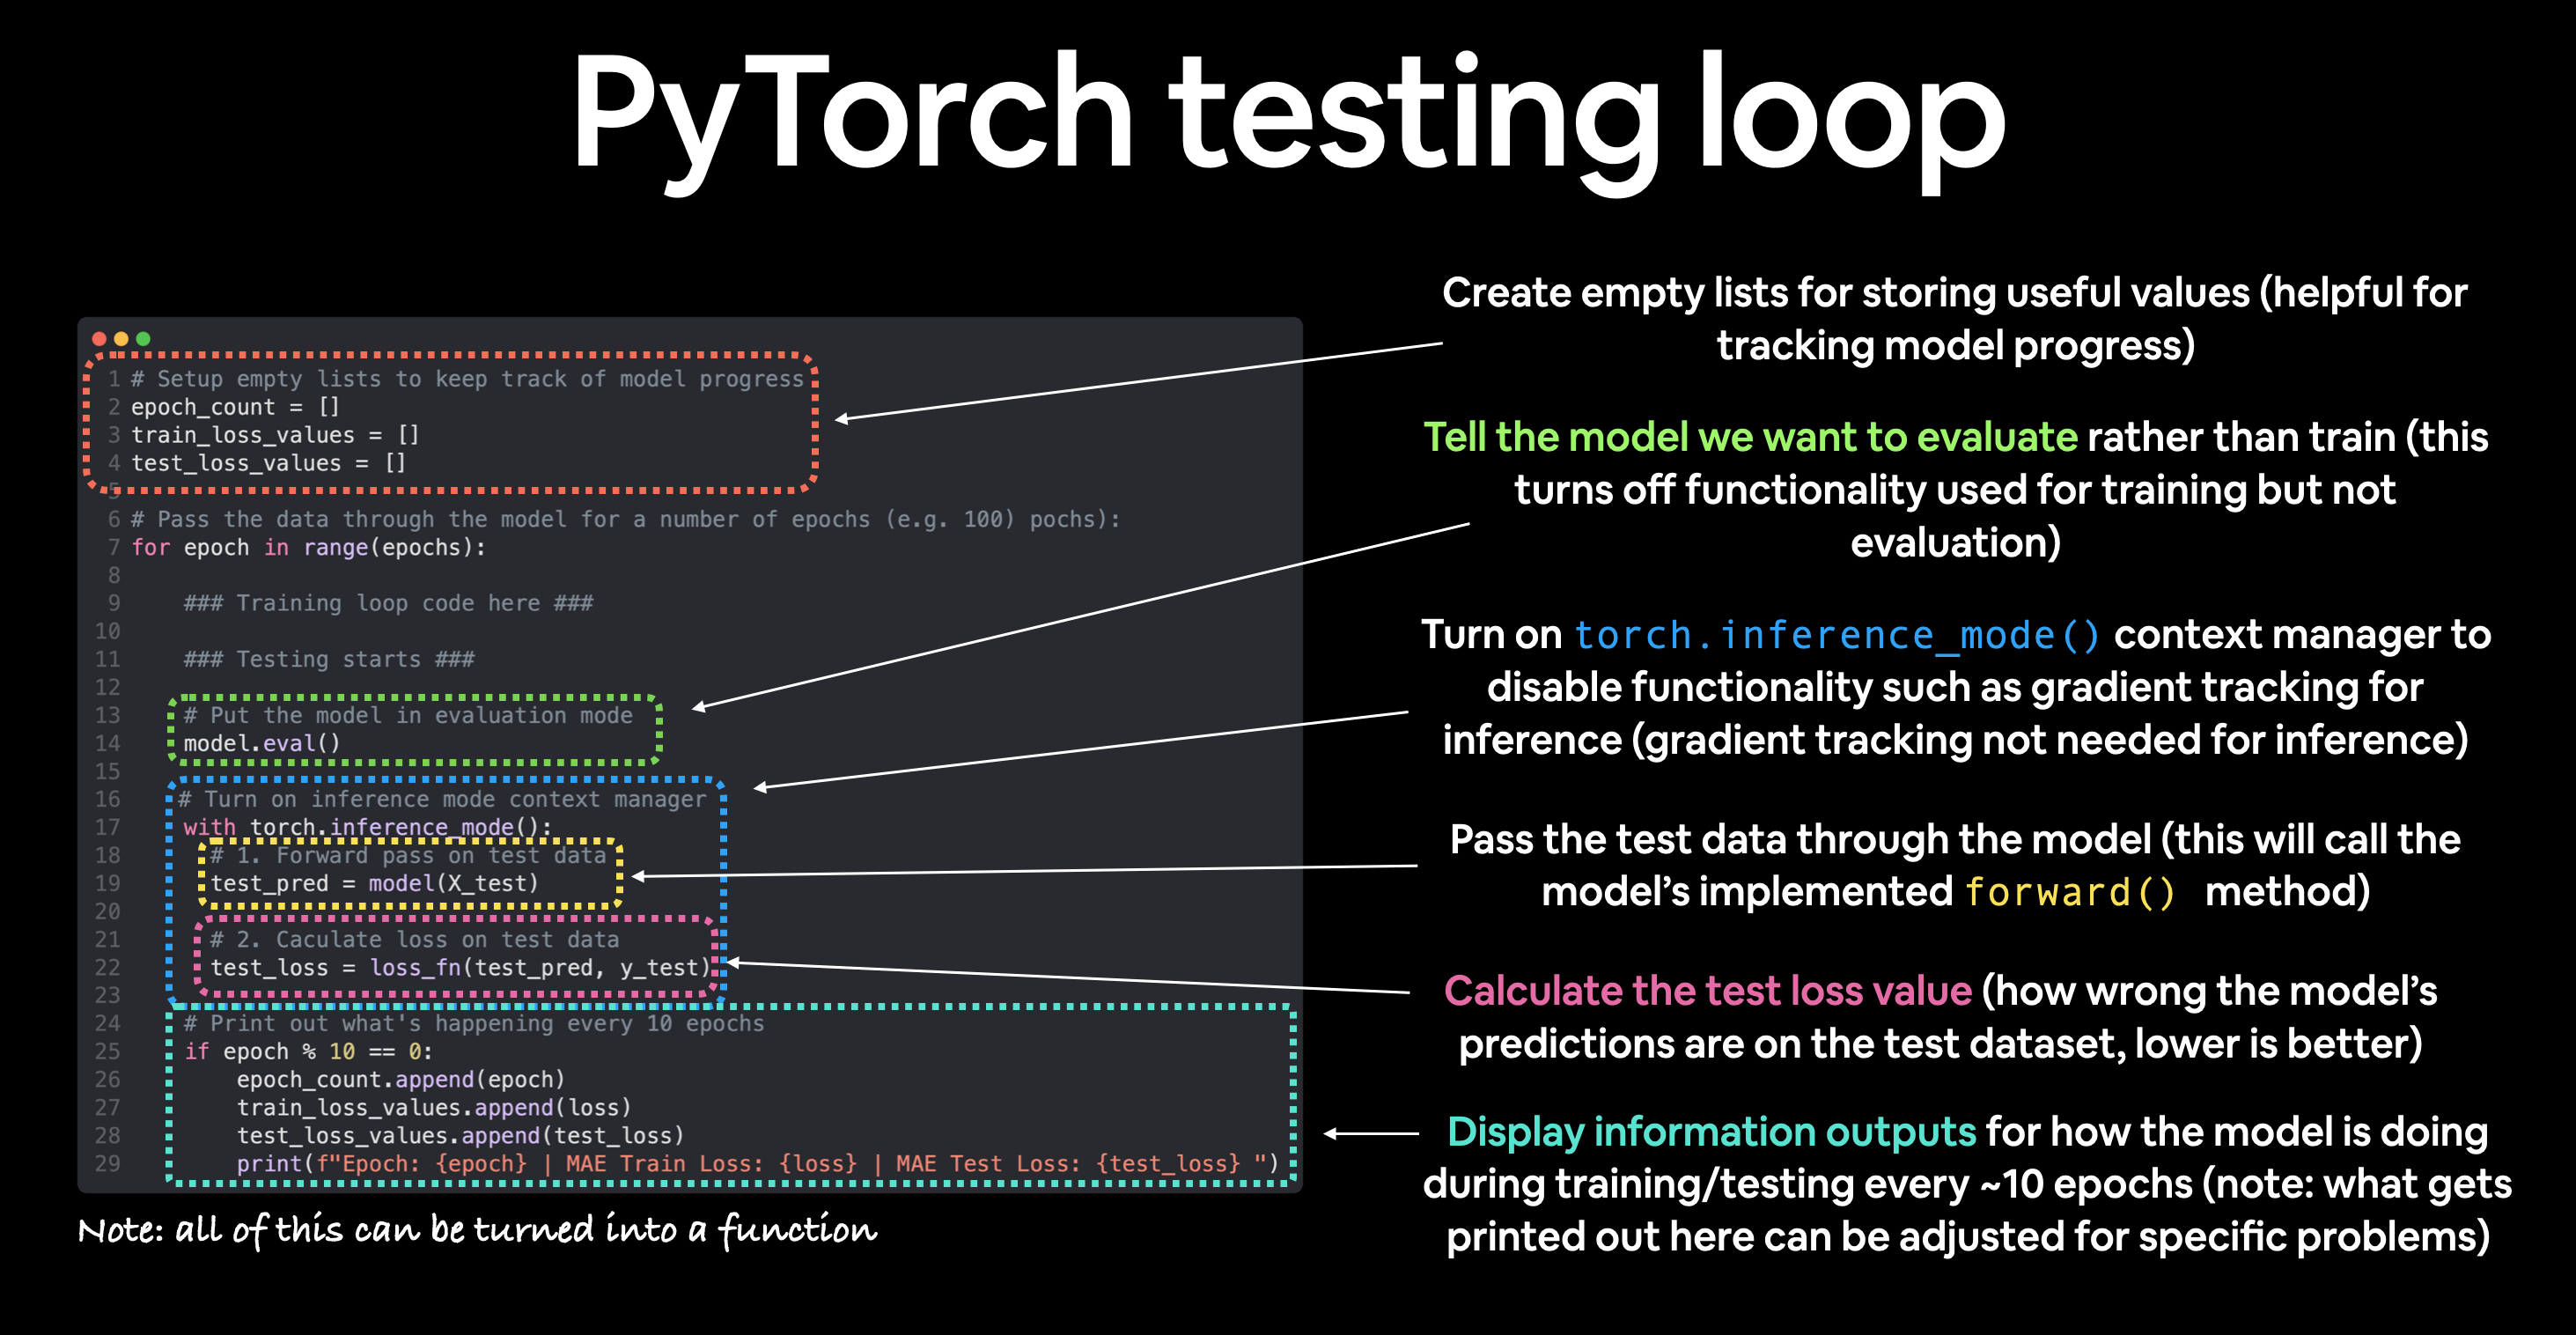
\includegraphics[width=0.7\linewidth]{figures/steps_test_torch}
		\end{figure}
		
	\end{block}
\end{frame}
%==========================================================================================
\begin{frame}
	\frametitle{Pytorch Regressão Linear - Fazendo predições com o Modelo Treinado}
	\begin{block}{Fazendo predições com o Modelo Treinado}
		\begin{itemize}
			\item[1] Mude para o modo de avaliação $model_0.eval()$
			\item[2] Faça as pervisões $y_preds = model_0(X_test)$
		\end{itemize}
	
	\end{block}
\end{frame}
%==========================================================================================
\begin{frame}
	\frametitle{Pytorch Regressão Linear - Salve o Modelo Treinado}
	\begin{block}{Salve o Modelo Treinado}
		Se você treinou um modelo PyTorch, é provável que queira salvá-lo e exportá-lo para algum lugar.
		
		Por exemplo, você pode treiná-lo no Google Colab ou em sua máquina local com uma GPU, mas agora gostaria de exportá-lo para algum tipo de aplicativo onde outras pessoas possam usá-lo.
		
		Ou talvez você queira salvar seu progresso em um modelo e voltar e carregá-lo mais tarde.
		\begin{itemize}
			\item[1] Salve o modelo treinado
			\item[2] Carregue o modelo salvo
			\item[3] Faça predições com o modelo carregado
		\end{itemize}
		
	\end{block}
\end{frame}
%==========================================================================================
\begin{frame}
	\frametitle{Pytorch Regressão Linear - Vamos criar o mesmo modelo de forma mais simples}
	\begin{block}{Novo Modelo}
		\begin{itemize}
			\item[1] Crie os dados para o modelo
			\item[2] Construa o modelo
			\item[3] Selecione a função de perda
			\item[4] Selecione o otimizador
			\item[5] Crie o loop de treinamento
			\item[6] Faça predições
			\item[7] Salve o modelo treinado
			\item[8] Carregue o modelo salvo
			\item[9] Faça predições com o modelo carregado
		\end{itemize}
		
	\end{block}
\end{frame}

%==========================================================================================
%==========================================================================================
\section{PyTorch Neural Network Classification}

\begin{frame}
	\frametitle{PyTorch Neural Network Classification}
	\begin{block}{PyTorch Neural Network Classification}
		\textbf{Binary classification:} Target can be one of two options, e.g. yes or no. Predict whether or not someone has heart disease based on their health parameters. 
		
		\textbf{Multi-class classification:} Target can be one of more than two options. Decide whether a photo of is of food, a person or a dog.
		
		\textbf{Multi-label classification:} Target can be assigned more than one option. Predict what categories should be assigned to a Wikipedia article (e.g. mathematics, science e philosohpy).
	\end{block}
\end{frame}
%==========================================================================================
\begin{frame}
	\frametitle{PyTorch Neural Network Classification}
	\begin{block}{PyTorch Neural Network Classification}
		O que vamos ver:
		\begin{itemize}
			\item Arquitetura de uma rede neural de classificação
			\item Preparando os dados de classificação binária
			\item Construindo um modelo de classificação PyTorch
			\item Ajustando o modelo aos dados (treinamento)
			\item Fazendo previsões e avaliando um modelo (inferência)
			\item Melhorando um modelo (de uma perspectiva de modelo)
			\item Não linearidade
			\item Replicando funções não lineares
			\item Juntando tudo com a classificação multiclasse
		\end{itemize}
	\end{block}
\end{frame}
%==========================================================================================
\begin{frame}
	\frametitle{PyTorch Neural Network Classification}
	\begin{block}{Arquitetura de uma rede neural de classificação}
		\begin{itemize}
			\item\textbf{Input layer shape (in\_features):} Same as number of features (e.g. 5 for age, sex, height, weight, smoking status in heart disease prediction)
			\item \textbf{Hidden layer(s):} Problem specific, minimum = 1, maximum = unlimited
			\item \textbf{Neurons per hidden layer:} Problem specific, generally 10 to 512
			\item \textbf{Output layer shape (out\_features):} 1 (one class or the other)
			\item \textbf{Hidden layer activation:} Usually ReLU (rectified linear unit) but can be many others
			\item \textbf{Output activation:} Sigmoid (torch.sigmoid in PyTorch)
			\item \textbf{Loss function:} Binary crossentropy (torch.nn.BCELoss in PyTorch)
			\item \textbf{Optimizer:} SGD (stochastic gradient descent), Adam (see torch.optim for more options)
		\end{itemize}
	\end{block}
\end{frame}
%==========================================================================================
\begin{frame}
	\frametitle{PyTorch Neural Network Classification}
	\begin{block}{Arquitetura de uma rede neural de classificação}
	Vamos ver isso no notebook, com o problema dos círculos!
	\begin{figure}
		\centering
		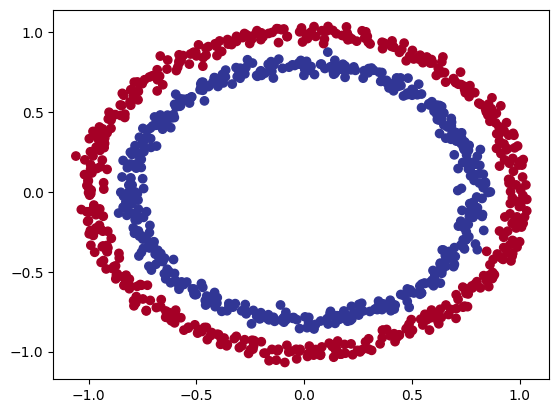
\includegraphics[width=0.4\linewidth]{figures/make_circle}
	\end{figure}
	Vamos ver este exemplo no TensorFlow Playground website \\
	\href{https://playground.tensorflow.org/}{\beamergotobutton{TensorFlow Playground website}} \\
	Vamos replicar este exemplo! \\
	Vamos descobrir como poderíamos construir uma rede neural PyTorch para classificar pontos em vermelho (0) ou azul (1).
	\end{block}
\end{frame}
%==========================================================================================
\begin{frame}
	\frametitle{PyTorch Neural Network Classification}
	\begin{block}{Arquitetura de uma rede neural de classificação}
		Os passos que vamos fazer:
		\begin{itemize}
			\item Vizualizar o shape dos dados $X.shape, y.shape$
			\item Transformar os dados em tensores: $torch.from\_numpy(X).type(torch.float)$
			\item Dividir em Train e Test: $train\_test\_split$
			\item Construir o modelo
			\item Fazer predições (sem treinamento)
			\item Escolher função de custo e Otimizador (no próximo slide)
			\item Desenvolver métrica de avaliação: $accuracy\_fn$
			\item Acessar: (https://datascience.stackexchange.com/a/31045)
		\end{itemize}
	\end{block}
\end{frame}
%==========================================================================================
\begin{frame}
	\frametitle{PyTorch Neural Network Classification}
	\begin{block}{Arquitetura de uma rede neural de classificação}
		Os passos que vamos fazer:
		% Please add the following required packages to your document preamble:
		% \usepackage{graphicx}
		\begin{table}[]
			\resizebox{\textwidth}{!}{%
				\begin{tabular}{|l|l|l|}
					\hline
					\textbf{Loss function/Optimizer}     & \textbf{Problem type}                    & \textbf{PyTorch Code}     \\ \hline
					Stochastic Gradient Descent (SGD) optimizer &
					Classification, regression, many others. &
					torch.optim.SGD() \\ \hline
					Adam Optimizer                       & Classification, regression, many others. & torch.optim.Adam()        \\ \hline
					Binary cross entropy loss &
					Binary classification &
					\begin{tabular}[c]{@{}l@{}}torch.nn.BCELossWithLogits\\ or torch.nn.BCELoss\end{tabular} \\ \hline
					Cross entropy loss                   & Multi-class classification               & torch.nn.CrossEntropyLoss \\ \hline
					Mean absolute error (MAE) or L1 Loss & Regression                               & torch.nn.L1Loss           \\ \hline
					Mean squared error (MSE) or L2 Loss  & Regression                               & torch.nn.MSELoss          \\ \hline
				\end{tabular}%
			}
		\end{table}
	\end{block}
\end{frame}
%==========================================================================================
\begin{frame}
	\frametitle{PyTorch Neural Network Classification}
	\begin{block}{Arquitetura de uma rede neural de classificação}
		Os passos que vamos fazer:
		\begin{itemize}
			\item Construir loop de treinamento
			\item Treinar o modelo 
			\item Analisar resultados: Se o modelo predizer todos os dados com a mesma classe a acurácia será 50\%. O que está acontecendo com o nosso modelo?
			\item Visualizar os nossos resultados: O lema do explorador de dados!
			\item Separação dos dados linearmente?
		\end{itemize}
	Vamos ver alguns ajustes que podemos fazer a seguir!
	\end{block}
\end{frame}
%==========================================================================================
\begin{frame}
	\frametitle{PyTorch Neural Network Classification}
	\begin{block}{Arquitetura de uma rede neural de classificação}
		A seguir estão algumas dicas para livrar seu modelo do problema de underfitting:
		\begin{itemize}
			\item Adicionar mais camadas
			\item Adicionar mais neurônios 
			\item Treinar por mais épocas
			\item Mudar as camadas de ativação
			\item Alterar o Learning Rate
			\item Alterar a função de perda
			\item Usar Transfering Learning
		\end{itemize}
	Esse tipo de alteração se referem as mudanças de hiperparâmetros! \\
	Vamos continuar tentando melhorar este modelo...
	\end{block}
\end{frame}
%==========================================================================================
\begin{frame}
	\frametitle{PyTorch Neural Network Classification}
	\begin{block}{Arquitetura de uma rede neural de classificação}
		\begin{itemize}
			\item Adicionar mais camadas
			\item Visualizar e analisar o resultado!
			\item Vamos construir um modelo não-linear!
			\item Vamos treinar o modelo
			\item Vamos analisar o desempenho do modelo
		\end{itemize}
	\end{block}
\end{frame}
%==========================================================================================
\begin{frame}
	\frametitle{PyTorch Neural Network Classification}
	\begin{block}{Arquitetura de uma rede neural de classificação}
		Vamos construir um modelo de classificação multi-classe
		\begin{itemize}
			\item Criar os dados
			\item Criar modelo - Selecionar Loss Function e Optimizer e Testá-lo
			\item Vamos treinar o modelo, testar e analisar o desempenho do modelo
		\end{itemize}
		\begin{figure}
			\centering
			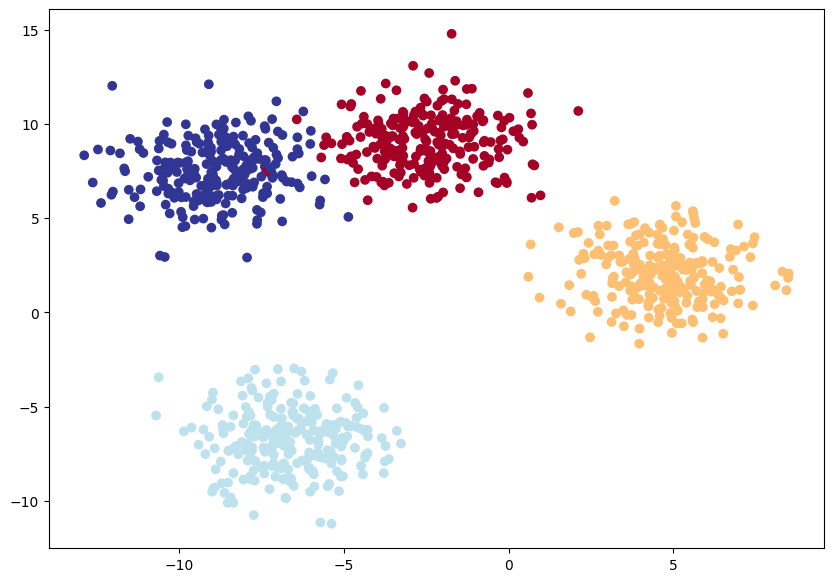
\includegraphics[width=0.3\linewidth]{figures/multiclass_example}
		\end{figure}
	\end{block}
\begin{alertblock}{Pergunta}
	Precisamos de não-linearidade para classificar estes dados?
\end{alertblock}
\end{frame}
%==========================================================================================
\begin{frame}
	\frametitle{PyTorch Neural Network Classification}
	\begin{block}{Métricas de avaliação do modelo}
	% Please add the following required packages to your document preamble:
	% \usepackage{graphicx}
	\begin{table}[]
		\resizebox{\textwidth}{!}{%
			\begin{tabular}{|l|l|l|}
				\hline
				\textbf{Metric} &
				\textbf{Defintion} &
				\textbf{PyTorch Code} \\ \hline
				Accuracy &
				\begin{tabular}[c]{@{}l@{}}Out of 100 predictions, how many does your model get correct?\\ E.g. 95\% accuracy means it gets 95/100 predictions correct.\end{tabular} &
				\begin{tabular}[c]{@{}l@{}}torchmetrics.Accuracy()\\ sklearn.metrics.accuracy\_score()\end{tabular} \\ \hline
				Precision &
				\begin{tabular}[c]{@{}l@{}}Proportion of true positives over total number of samples.\\ Higher precision leads to less false positives (model predicts 1 when it should've been 0).\end{tabular} &
				\begin{tabular}[c]{@{}l@{}}torchmetrics.Precision()\\ sklearn.metrics.precision\_score()\end{tabular} \\ \hline
				Recall &
				\begin{tabular}[c]{@{}l@{}}Proportion of true positives over total number of true positives and false negatives\\ (model predicts 0 when it should've been 1). Higher recall leads to less false negatives.\end{tabular} &
				\begin{tabular}[c]{@{}l@{}}torchmetrics.Recall()\\ sklearn.metrics.recall\_score()\end{tabular} \\ \hline
				F1-score &
				Combines precision and recall into one metric. 1 is best, 0 is worst. &
				\begin{tabular}[c]{@{}l@{}}torchmetrics.F1Score()\\ sklearn.metrics.f1\_score()\end{tabular} \\ \hline
				Confusion matrix &
				\begin{tabular}[c]{@{}l@{}}Compares the predicted values with the true values in a tabular way, if 100\% correct,\\ all values in the matrix will be top left to bottom right (diagnol line).\end{tabular} &
				\begin{tabular}[c]{@{}l@{}}torchmetrics.ConfusionMatrix\\ sklearn.metrics.plot\_confusion\_matrix()\end{tabular} \\ \hline
				Classification report &
				Collection of some of the main classification metrics such as precision, recall and f1-score. &
				sklearn.metrics.classification\_report() \\ \hline
			\end{tabular}%
		}
	\end{table}
	\end{block}
\end{frame}
%==========================================================================================

\section{PyTorch Computer Vision}


%==========================================================================================
\begin{frame}
	\frametitle{PyTorch Computer Vision}
	\begin{block}{Computer Vision}
		Vamos utilizar o notebook 09
			\begin{itemize}
			\item Arte de ensinar um computador a ver
			\item Modelo para classificar se uma foto é de um gato ou de um cachorro (classificação binária)
			\item Ou se a foto é de um gato, cachorro ou galinha (classificação multiclasse)
			\item Ou identificar onde um carro aparece em um quadro de vídeo (detecção de objeto)
			\item Ou descobrir onde diferentes objetos em uma imagem podem ser separados (segmentação panóptica)
			\item Usado no seu celular, câmera, indústria, medicina, etc.
		\end{itemize}
	\end{block}
\end{frame}

%==========================================================================================
\begin{frame}
	\frametitle{PyTorch Computer Vision}
	\begin{figure}
		\centering
		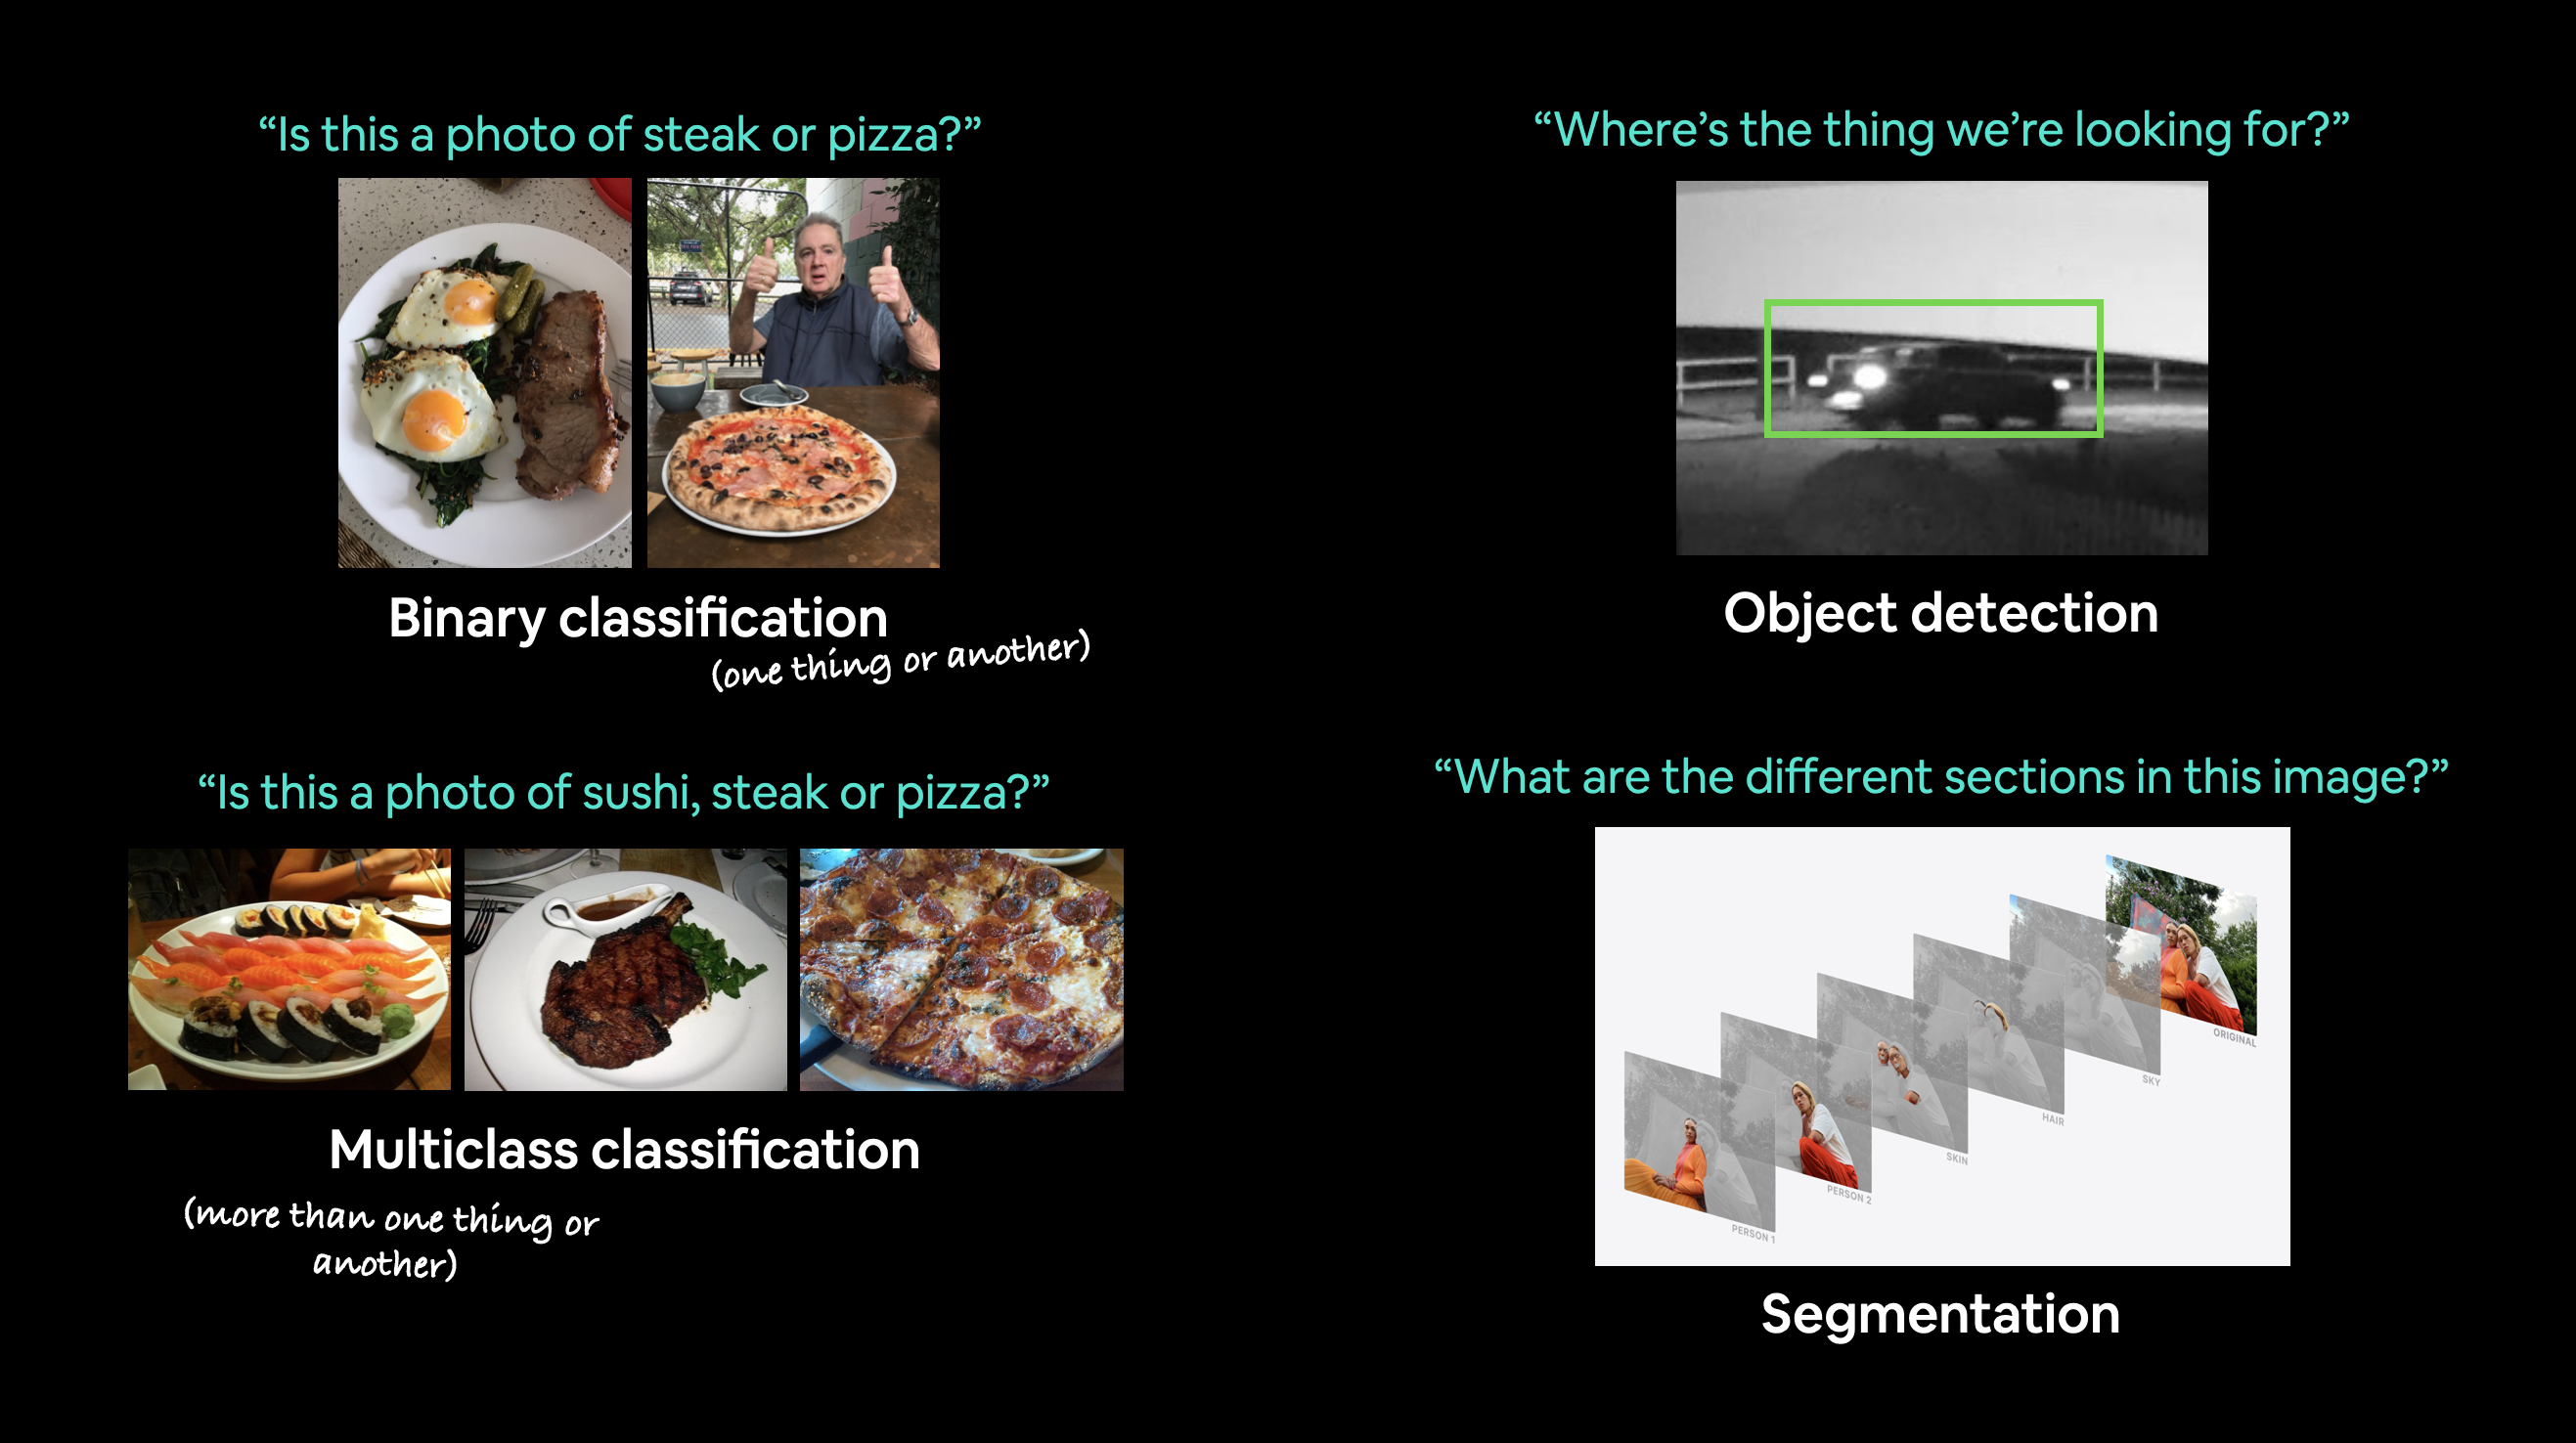
\includegraphics[width=1\linewidth]{figures/vision_comp}
	\end{figure}
	
\end{frame}
%==========================================================================================
\begin{frame}
	\frametitle{PyTorch Computer Vision}
	\begin{block}{Computer Vision - O que vamos fazer}
		\begin{itemize}
			\item Adquirindo o Dataset Fashion:
			\begin{itemize}
				\item Escala de cinza
				\item 10 tipos de roupas
			\end{itemize}
			\item Verificar a primeira amostra de dados de treinamento
			\item Vizualizar o Input e Output dos dados:
			\begin{itemize}
				\item Ordem dos dados no tensor: CHW (color channels first) or HWC (color channels last)
				\item NCHW - Número de imagens, Ex: batch\_size=32 - [32, 1, 28, 28]
			\end{itemize}
			\item Visualizar total de imagens de treinamento (60000) e teste (10000)
			\item Visualizar as 10 classes
			\item Visualizar uma imagem, transforma-la na escala de cinza
			\item Visualizar mais exemplares de imagens
		\end{itemize}
	\end{block}
\end{frame}
%==========================================================================================
\begin{frame}
	\frametitle{PyTorch Computer Vision}
	\begin{block}{Computer Vision - O que vamos fazer}
		\begin{itemize}
			\item Prepare o dataloader
			\begin{itemize}
				\item Usado para carregar as imagens para o modelo
				\item Treinamento e Inferência
				\item Divide o nosso dataset em Batchs ou Mini-Batches
			\end{itemize}
			\item Montar o modelo Base
			\item Vizualizar o Input e Output dos dados:
			\begin{itemize}
				\item Ordem dos dados no tensor: CHW (color channels first) or HWC (color channels last)
				\item NCHW - Número de imagens, Ex: batch\_size=32 - [32, 1, 28, 28]
			\end{itemize}
			\item Visualizar total de imagens de treinamento (60000) e teste (10000)
			\item Visualizar as 10 classes
			\item Visualizar uma imagem, transforma-la na escala de cinza
			\item Visualizar mais exemplares de imagens
		\end{itemize}
	\end{block}
\end{frame}
%==========================================================================================
\begin{frame}
	\frametitle{PyTorch Computer Vision}
	\begin{block}{Computer Vision - O que vamos fazer}
		\begin{itemize}
			\item Construir o modelo base
			\begin{itemize}
				\item Modelo simples
				\item Melhorar o modelo subsequentemente
				\item MODELO: flatten - Linear - Linear
			\end{itemize}
			\item Montar o modelo Base
			\item Selecionar a função de perda, otimizador e métricas de avaliação
		\end{itemize}
	\end{block}
\end{frame}
%==========================================================================================

\begin{frame}
	\frametitle{PyTorch Computer Vision}
	\begin{block}{Computer Vision - O que vamos fazer}
		\begin{itemize}
			\item Criar uma função para medir a velocidade da execução na CPU vs GPU
			\item CPU:
			\begin{itemize}
				\item Treinar e Testar
			\end{itemize}
			\item GPU:
			\begin{itemize}
				\item Setar ambiente de execução para GPU
				\item Construir um modelo melhor com não linearidade
				\item Selecionar a função de perda, otimizador e métricas de avaliação
				\item Funcionalização de loops de treinamento e teste
				\item Treinar e comparar a velocidade de execução vs CPU
			\end{itemize}
		\end{itemize}
	\end{block}
	\begin{alertblock}{Nota}
		Note que, Construir um modelo melhor com não linearidade piorou nossos resultados, aconteceu overfitting. \\
		Exercício: evitar overfitting mudando o modelo ou com conjunto de dados maior
	\end{alertblock}
\end{frame}
%==========================================================================================

\begin{frame}
	\frametitle{PyTorch Computer Vision}
	\begin{block}{Computer Vision - Redes Neurais Convolucionais}
		\begin{itemize}
			\item CNN ou ConvNet \href{https://en.wikipedia.org/wiki/Convolutional_neural_network}{\beamergotobutton{CNN}} 
			\item Identifica padrões em imagens
			\item Vamos conhecer o CNN EXPLAINER \href{https://poloclub.github.io/cnn-explainer/}{\beamergotobutton{CNN Site}} 
			\begin{itemize}
				\item Input layer - [Convolutional layer - activation layer - pooling layer] - Output layer (Bloco)
			\end{itemize}
			\item Vamos criar um modelo CNN conforme o visto no site CNN Explainer
			\item O que é a convolução 2D: $nn.conv2d()$? ...
		\end{itemize}
	\end{block}
\end{frame}
%==========================================================================================
\begin{frame}
	\frametitle{PyTorch Computer Vision}
	\begin{block}{Computer Vision - Redes Neurais Convolucionais}
		Vamos ver a algumas características da convolução 2D na prática:
		\begin{itemize}
			\item in\_channels (int) - Número de canais na imagem de entrada.
			\item out\_channels (int) - Número de canais produzidos pela convolução.
			\item kernel\_size (int ou tupla) - Tamanho do kernel/filtro de convolução.
			\item stride (int ou tupla, opcional) - O tamanho do passo que o kernel convolutivo leva por vez. Padrão: 1.
			\item padding (int, tuple, str) - Padding adicionado a todos os quatro lados da entrada. Padrão: 0.
			\item Gif da Conv2d\href{https://github.com/mafaldasalomao/pavic_treinamento_ml/blob/main/Machine_Learning/figures/03-conv2d-layer.gif?raw=true}{\beamergotobutton{Conv2d}} 
			\item Vamos alterar os parâmetros da Conv2d
		\end{itemize}
	\end{block}
\end{frame}
%==========================================================================================
\begin{frame}
	\frametitle{PyTorch Computer Vision}
	\begin{block}{Computer Vision - Redes Neurais Convolucionais}
		\begin{itemize}
			\item Selecione a função de Perda e Otimizador
			\item Vamos treinar o modelo
			\item Vamos avaliar o modelo
			\item Vamos comparar o desempenhos dos 3 modelos desenvolvidos:
			\begin{itemize}
				\item model\_0 - nosso modelo básico com duas camadas nn.Linear().
				\item model\_1 - a mesma configuração do nosso modelo base, exceto com as camadas nn.ReLU() entre as camadas nn.Linear().
				\item model\_2 - nosso primeiro modelo CNN que imita a arquitetura TinyVGG no site CNN Explainer.
			\end{itemize}
			\item Vamos fazer mais predições com nosso melhor modelo
			\item Construir a matriz de confusão
			\item Salvar, carregar e testar nosso melhor modelo
		\end{itemize}
	\end{block}
\end{frame}


%==========================================================================================
\section{PyTorch Custom Datasets}
\begin{frame}
	\frametitle{PyTorch Custom Datasets}
	\begin{block}{Custom Datasets}
		
		\begin{itemize}
			\item Um conjunto de dados personalizado é uma coleção de dados relacionados a um problema específico no qual você está trabalhando.
			\item Por exemplo, se estivéssemos criando um aplicativo de classificação de imagens de alimentos, nosso conjunto de dados personalizado poderia ser imagens de alimentos.
			\item Ou, se estivéssemos tentando criar um modelo para classificar se uma avaliação baseada em texto em um site era positiva ou negativa.
			\item Ou, se estivéssemos tentando criar um aplicativo de classificação de som, nosso conjunto de dados personalizado poderia ser amostras de som junto com seus rótulos de amostra.
			\item Ou, se estivéssemos tentando criar um sistema de recomendação para clientes que compram coisas em nosso site, nosso conjunto de dados personalizado pode ser exemplos de produtos que outras pessoas compraram.
		\end{itemize}
	\end{block}
\end{frame}
%==========================================================================================
\begin{frame}
	\frametitle{PyTorch Custom Datasets}
	\begin{block}{Custom Datasets}
		O que vamos fazer:
		\begin{itemize}
			\item Importar cuda
			\item Vamos adquirir os dados:
			\begin{itemize}
				\item Usaremos um subconjunto do dataset \href{https://data.vision.ee.ethz.ch/cvl/datasets_extra/food-101/}{\beamergotobutton{Food-101}} 
				\item 1000 imagens de 101 tipos de comidas diferentes = 101.000 imagens (75.750 treinamento e 25250 para teste)
				\item Qual a complexidade deste modelo para predizer 101 tipos de comidas diferentes?
			\end{itemize}
			\item Pré-processamento dos dados - preparação
			\item Visualize uma imagem
			\item Transforme os dados no tensor do Pytorch
		\end{itemize}
	\end{block}
\end{frame}

%==========================================================================================
\begin{frame}
	\frametitle{PyTorch Custom Datasets}
	\begin{block}{Custom Datasets}
		O que vamos fazer:
		\begin{itemize}
			\item Transforme os dados no tensor do Pytorch
			\item Vamos ver o funcionamento do torchvision.transforms:
			\begin{itemize}
				\item Manipulação dos dados
				\item Data augmentation (Redimensionamento, Flip, e transformação para tensor)
				\item Todas as alterações são compiladas utilizando o $torchvision.transforms.Compose()$
			\end{itemize}
			\item Vamos construir uma função que mostrará mais imagens
		\end{itemize}
	\end{block}
\end{frame}

%==========================================================================================
\begin{frame}
	\frametitle{PyTorch Custom Datasets - Opções para carregar o dataset}
	\begin{block}{Opção 1: ImageFolder}
		Muito utilizado para carregar datasets de classificação $torchvision.datasets.ImageFolder$
		\begin{itemize}
			\item Vamos carregar as imagens utilizando o ImageFolder
			\item Carregar os dados para o DataLoader  
			\begin{itemize}
				\item Deixa os dados iteráveis
				\item Deixa os dados ordenados em \textit{sample} e \textit{targets} 
			\end{itemize}
		\end{itemize}
	\end{block}
\end{frame}
%==========================================================================================
\begin{frame}
	\frametitle{PyTorch Custom Datasets - Opções para carregar o dataset}
	\begin{block}{Opção 2: Carregando o dataset com Custom Dataset}
		Carregue seu dataset personalizado
		\begin{itemize}
			\item Usado quando o ImageFolder não for útil
			\item Usado em problemas específicos
			\begin{itemize}
				\item $os$ do Python para lidar com diretórios (nossos dados são armazenados em diretórios).
				\item $pathlib$ do Python para lidar com caminhos de arquivo (cada uma de nossas imagens tem um caminho de arquivo exclusivo).
				\item $torch$ para todas as coisas PyTorch.
				\item $Image$ PIL para carregar imagens.
				\item $torch.utils.data.Dataset$ para criar uma subclasse e criar nosso próprio Dataset personalizado
				\item $torchvision.transforms$ para transformar nossas imagens em tensores.
				\item Vários tipos do módulo $typing$ do Python para adicionar dicas de tipo ao nosso código
			\end{itemize}
		\end{itemize}
	\end{block}
\end{frame}
%==========================================================================================
\begin{frame}
	\frametitle{PyTorch Custom Datasets - Opções para carregar o dataset}
	\begin{block}{Opção 2: Carregando o dataset com Custom Dataset}
		Vamos criar nosso dataset customizado
		\begin{itemize}
			\item Importe as bibliotecas
			\item Crie uma função para adquirir o nome das classes do seu dataset
			\item Crie a Classe para o Dataset Customizado
			\item Crie os transformers
			\item Carregue as imagens utilizando a função criada
			\item Vamos ver como estão os dados
		\end{itemize}
	\end{block}
\end{frame}
%==========================================================================================
\begin{frame}
	\frametitle{PyTorch Custom Datasets}
	\begin{block}{PyTorch Custom Datasets}
		\begin{itemize}
			\item Vamos criar uma função para mostrar imagens aleatórias
			\item Mostre as imagens utilizando a função criada acima
			\item Vamos carregar nossos dados no $Dataloader$
		\end{itemize}
	\end{block}
\end{frame}

%==========================================================================================
\begin{frame}
	\frametitle{PyTorch Custom Datasets}
	\begin{block}{Outras formas de transforms (data augmentation)}
		A documentação dos transformers pode ser acessado: \href{https://pytorch.org/vision/stable/transforms.html}{\beamergotobutton{torchvision.transforms}} \\
		Um dos objetivos de se utilizar \textit{data augmentation} é \textbf{artificialmente} aumentar a diversidade e tamanho do nosso conjunto de treinamento.
		Dessa forma, esperamos que o modelo passe a generalizar mais os resultados (padrão não vistos).\\
		Neste link podemos ver alguns exemplos: \href{https://pytorch.org/vision/stable/auto_examples/plot_transforms.html\#illustration-of-transforms}{\beamergotobutton{Exemplos}}. \\
		How to Train State-Of-The-Art Models Using TorchVision’s Latest Primitives \href{https://pytorch.org/blog/how-to-train-state-of-the-art-models-using-torchvision-latest-primitives/\#break-down-of-key-accuracy-improvements}{\beamergotobutton{Acessar}} 
	\end{block}
	\begin{alertblock}{Atenção}
		Normalmente usamos augmentation no conjunto de treinamento, para que melhore o desempenho no conjunto de teste. Mas, alterar o tamanho das imagens de treinamento é considerado aumento de dados? Altera a performance?
	\end{alertblock}
\end{frame}
%==========================================================================================
\begin{frame}
	\frametitle{PyTorch Custom Datasets}
	\begin{block}{Model 0: TunyVGG \textbf{SEM} data augmentation}
		\begin{itemize}
			\item Vamos classificar nosso dataset em pizza, sushi ou bife
			\item Image size: (64, 64)
			\item Criar os transformers e carregar os dados para o Model 0:
			\begin{itemize}
				\item Carregar as imagens utilizando $torchvision.datasets.ImageFolder()$
				\item Carregar no DataLoader $torch.utils.data.DataLoader()$ 
				\item batch\_size=32
			\end{itemize}
			\item Vamos criar a classe do modelo TinyVGG
		\end{itemize}
	\end{block}
\end{frame}           

%==========================================================================================
%==========================================================================================
\begin{frame}
	\frametitle{PyTorch Custom Datasets}
	\begin{block}{Model 0: TunyVGG sem data augmentation}
		Tente um forward em uma única imagem (para testar o modelo)
		\begin{itemize}
			\item Obtenha um lote de imagens e rótulos do DataLoader
			\item Obtenha uma única imagem do lote e unsqueeze() a imagem para que ela tenha um tamanho de lote de 1 (para que sua forma se ajuste ao modelo).
			\item Realize a inferência em uma única imagem (certificando-se de enviar a imagem para o dispositivo de destino).
			\item Imprima o que está acontecendo e converta os logits brutos de saída do modelo em probabilidades de previsão com torch.softmax() (já que estamos trabalhando com dados multiclasse) e converta as probabilidades de previsão em rótulos de previsão com torch.argmax( ).
		\end{itemize}
	\end{block}
\end{frame}  
%==========================================================================================
\begin{frame}
	\frametitle{PyTorch Custom Datasets}
	\begin{block}{Model 0: TunyVGG sem data augmentation}
		\begin{itemize}
			\item Use torchinfo para ter uma ideia das formas passando pelo nosso modelo
			\item Vamos criar o Loop de treinamento e teste (vamos fazer 3 funções)
			\begin{itemize}
				\item train\_step(): receberá: modelo, Dalatoader, Loss Function, Otimizador e treinará o modelo
				\item test\_step(): receberá: modelo, Dalatoader, Loss Function, Otimizador e avaliará o modelo
				\item train(): Juntará as duas funções anteriores com um número de épocas e retornará um dicionário com resultados
			\end{itemize}
			\item Vamos treinar e avaliar o modelo com as funções criadas: 5 épocas, Adam e CrossEntropyLoss serão os hiperparâmetros utilizados
			\item vamos plotar as curvas de perda do modelo
		\end{itemize}
	\end{block}
\end{frame} 
%==========================================================================================
%==========================================================================================
\begin{frame}
	\frametitle{PyTorch Custom Datasets}
	\begin{block}{Model 0: TunyVGG sem data augmentation}
		Overfitting, como evitar?
		\begin{figure}
			\centering
			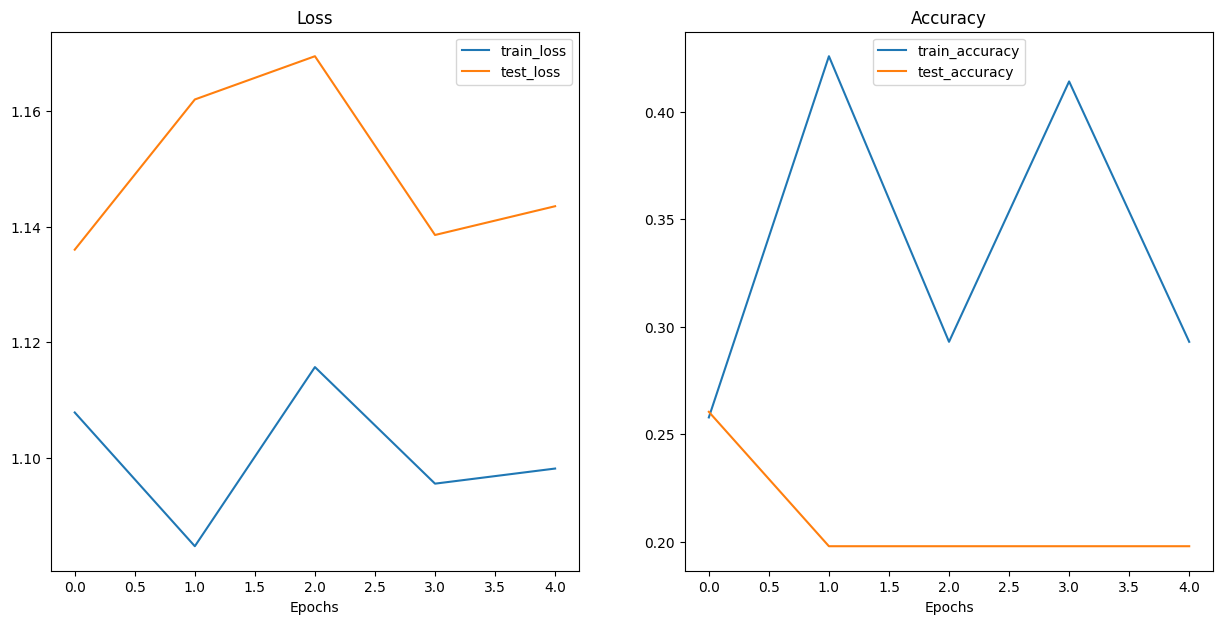
\includegraphics[width=1\linewidth]{figures/acc_curve_over}
		\end{figure}

	\end{block}
\end{frame} 
%==========================================================================================
\begin{frame}
	\frametitle{PyTorch Custom Datasets}
	\begin{block}{Model 0: TunyVGG sem data augmentation}
		Overfitting, como evitar?		
		\begin{itemize}
			\item Mais dados
			\item Simplificar o modelo
			\item Usar data augmentation
			\item Usar Transfer Learning
			\item Dropout
			\item Leraning rate decay
			\item Early stopping
		\end{itemize}
	\end{block}
\end{frame} 
%==========================================================================================
\begin{frame}
	\frametitle{PyTorch Custom Datasets}
	\begin{block}{Model 0: TunyVGG \textbf{COM} data augmentation}
		\begin{itemize}
			\item Vamos classificar nosso dataset em pizza, sushi ou bife
			\item Image size: (64, 64)
			\item Criar os transformers e carregar os dados para o Model 1:
			\begin{itemize}
				\item Carregar as imagens utilizando $torchvision.datasets.ImageFolder()$
				\item Carregar no DataLoader $torch.utils.data.DataLoader()$ 
				\item batch\_size=32
			\end{itemize}
			\item Vamos criar o modelo
			\item Vamos treinar o modelo e analisar a curva de perda
			\item Vamos comparar os resultados dos modelos
		\end{itemize}
	\end{block}
\end{frame}           

%===================================================================================
%==========================================================================================
\begin{frame}
	\frametitle{PyTorch Custom Datasets}
	\begin{block}{Model 0: TunyVGG \textbf{COM} data augmentation}
		\begin{itemize}
			\item Vamos classificar nosso dataset em pizza, sushi ou bife
			\item Image size: (64, 64)
			\item Criar os transformers e carregar os dados para o Model 1:
			\begin{itemize}
				\item Carregar as imagens utilizando $torchvision.datasets.ImageFolder()$
				\item Carregar no DataLoader $torch.utils.data.DataLoader()$ 
				\item batch\_size=32
			\end{itemize}
			\item Vamos criar o modelo
			\item Vamos treinar o modelo e analisar a curva de perda
			\item Compararemos os modelos
			\item Faremos a predição de uma imagens, e com uma imagem do seus arquivos pessoais
			Criaremos uma função de predição e plot da imagem de teste
		\end{itemize}
	\end{block}
\end{frame}           

%===================================================================================
\section{PyTorch Transformando o código em módulos}
\begin{frame}
	\frametitle{PyTorch Transformando o código em módulos}
	\begin{block}{PyTorch Transformando o código em módulos}
		\begin{figure}
			\centering
			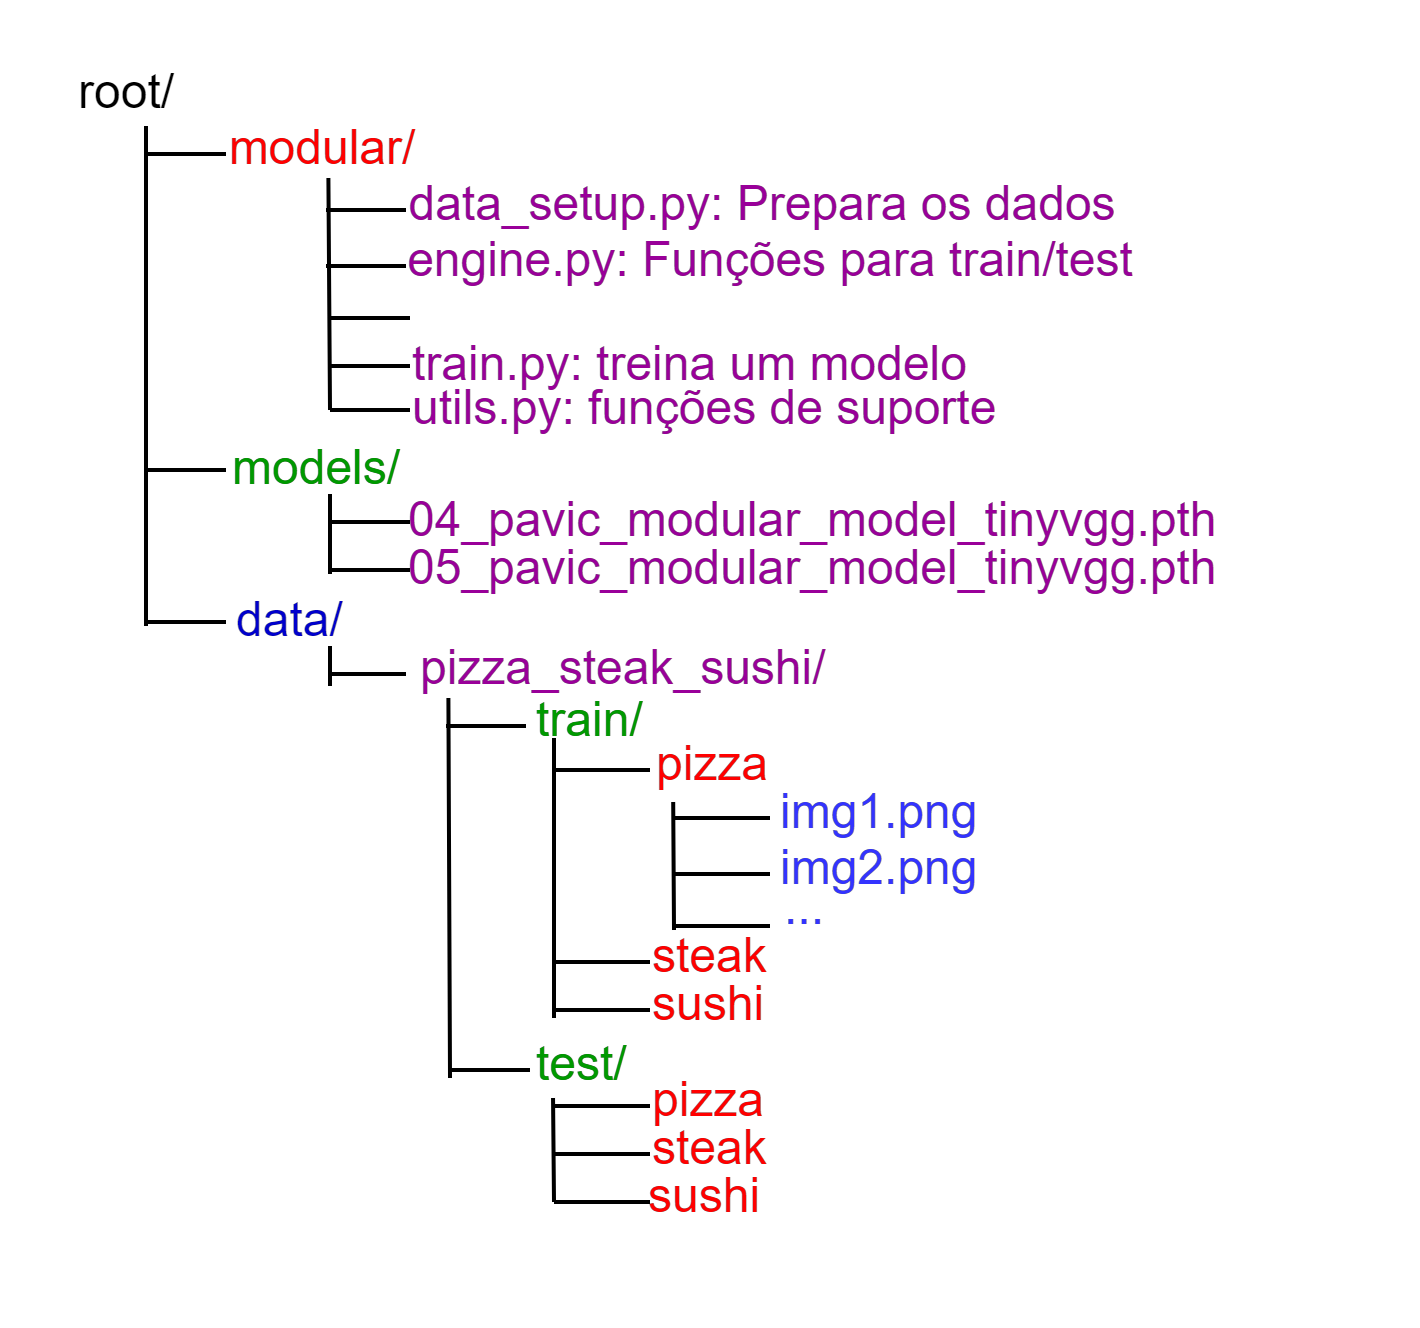
\includegraphics[width=0.7\linewidth]{figures/modular}
		\end{figure}
	\end{block}
\end{frame}
%===================================================================================
\begin{frame}
	\frametitle{PyTorch Transformando o código em módulos}
	\begin{block}{Na linha de comando: Comand line}
		train.py -model MODEL\_NAME -batch\_size BATCH\_SIZE -lr LEARNING\_RATE -num\_epochs NUM\_EPOCHS
	\end{block}
	\begin{block}{Cell mode}
		O notebook aqui utilizado será disponibilizado baseado no notebook do tópico anterior, porém enxuto.
		\begin{itemize}
			\item O que é um notebook cell mode? É o que vimos até agora no curso (texto/códigos)
			\item Vamos executar esse notebook normalmente:
			\begin{itemize}
				\item[1] Aquisição dos dados
				\item[2] Criar Datasets e DataLoaders
				\item[3] Construir o model0 (TinyVGG)
				\item[4] Criar as funções train\_step() e test\_step() e train() para combiná-las
				\item[5] Criar uma função para salvar o modelo
				\item[6] Treinar, avaliar e salvar o modelo
			\end{itemize}
		\end{itemize}
	\end{block}
\end{frame}
%===================================================================================
\begin{frame}
	\frametitle{PyTorch Transformando o código em módulos}
	\begin{block}{Script mode}
		\begin{itemize} 
			\item As células específicas são transformadas em scripts de python
			\item Quando quisermos executar o código faremos:
			\begin{itemize}
				\item !python going\_modular/train.py para executar linha de comando em uma célula do colab
				\item python going\_modular/train.py se formos executar no CMD ou terminal diretamente
			\end{itemize}
		\end{itemize}
	\end{block}
	\begin{example}
		\textit{\%\%writefile hello\_world.py \\
		print("hello world, machine learning is fun!")} \\
		Será escrito em um arquivo  \textit{hello\_word.py} \\
		Se digitarmos no terminar: \textit{python hello\_world.py} \\
		A saída será: \textit{hello world, machine learning is fun!}
	\end{example}
\end{frame}
%===================================================================================
\begin{frame}
	\frametitle{PyTorch Transformando o código em módulos}
	\begin{block}{A estrutura que montaremos seguirá este padrão}
		\begin{figure}
			\centering
			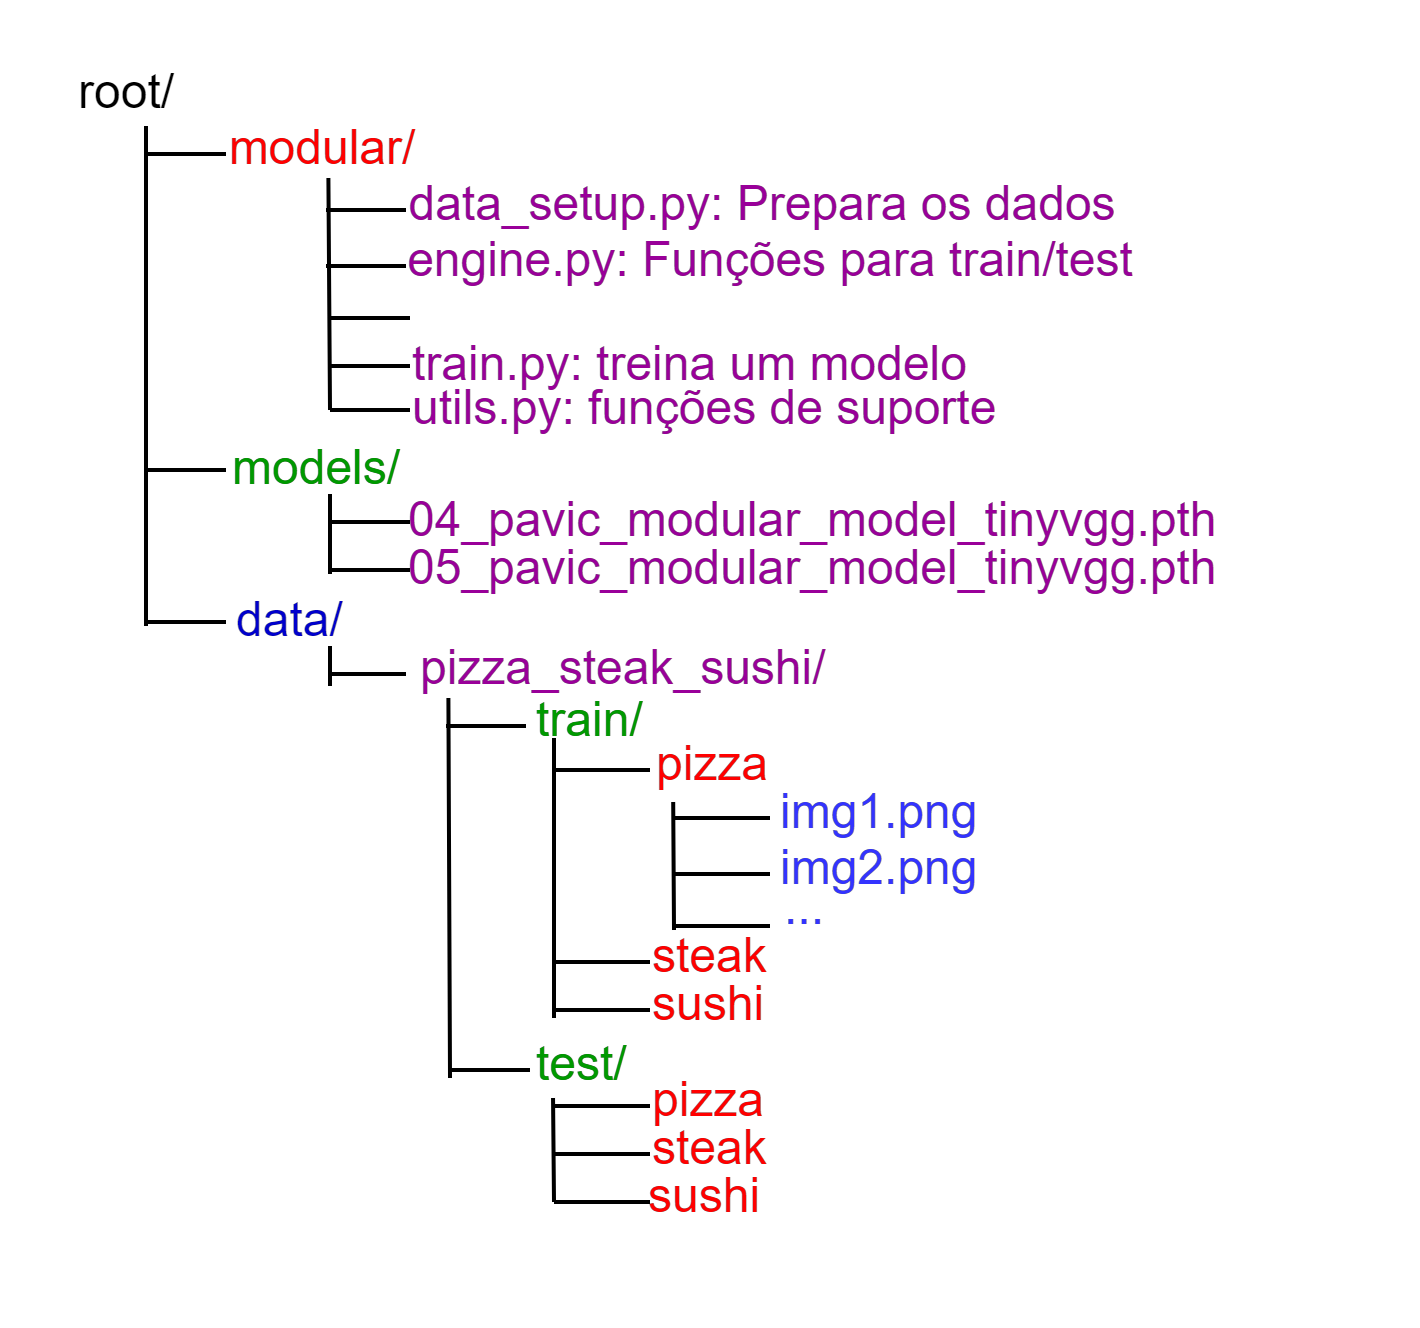
\includegraphics[width=0.7\linewidth]{figures/modular}
		\end{figure}
	\end{block}
\end{frame}
%===================================================================================
\begin{frame}
	\frametitle{PyTorch Transformando o código em módulos}
	\begin{block}{Transformando o cell mode para Script mode}
		\begin{itemize}
			\item[0] Criar pasta ``going\_modular''
			\item[1] Aquisição dos dados
			\item[2] Criar Datasets e DataLoaders
			\item[3] Criar Datasets e DataLoaders no \textbf{script mode}
			\item[4] Construir o model0 (TinyVGG)
			\item[5] Construir o model0 (TinyVGG) no \textbf{script mode}
			\item[6] Criar as funções train\_step() e test\_step() e train() para combiná-las
			\item[7] Criar as funções train\_step() e test\_step() e train() \textbf{script mode}
			\item[8] Criar uma função para salvar o modelo
			\item[9] Criar uma função para salvar o modelo \textbf{script mode}
			\item[10] Treinar, avaliar e salvar o modelo
			\item[11] Treinar, avaliar e salvar o modelo \textbf{script mode}
		\end{itemize}
	\end{block}
\end{frame}





%===================================================================================
\section{PyTorch Transfer Learning}



\begin{frame}
	\frametitle{PyTorch Transfer Learning}
	\begin{block}{PyTorch Transfer Learning}
		\begin{itemize}
			\item Permite pegar padrões (pesos) que outro modelo aprendeu e aplicar em um problema específico
			\item Ex: Modelo treinado no ImageNet para usar no FoodVision Minimodelo
			\item Permite melhorar um modelo existente em problemas semelhantes
			\item Melhora o treinamento e consequentemente os resultados
			\item Benéfica ao tempo e custo de treinamento
			\item Jeremy Howard: ``As coisas que realmente fazem a diferença (aprendizado por transferência), se pudermos fazer melhor no aprendizado por transferência, é essa coisa que muda o mundo. De repente, muito mais pessoas podem fazer um trabalho de classe mundial com menos recursos e menos dados''
		\end{itemize}
	\end{block}
\end{frame}    
%==========================================================================================
\begin{frame}
	\frametitle{PyTorch Transfer Learning}
	\begin{block}{PyTorch Transfer Learning}
		Os passos que vamos fazer:
		\begin{itemize}
			\item[1] Vamos configurar o ambiente do colab para usar GPU e baixar o repositório modular
			\item[2] Obter dados
			\item[3] Criar conjunto de dados e Dataloader
			\begin{itemize}
				\item Creating a transform for torchvision.models (manual creation)
				\item Creating a transform for torchvision.models (auto creation)
			\end{itemize}
			\item[4] Adquirir modelo pré-treinado
			\begin{itemize}
				\item Qual modelo escolher?
				\item Configurando um modelo pré treinado
				\item Olhando mais informações com o summary do nosso modelo `torchinfo.summary()`
			\end{itemize}
		\end{itemize}
	\end{block}
\end{frame}    
%==========================================================================================
%==========================================================================================
\begin{frame}
	\frametitle{PyTorch Transfer Learning}
	\begin{block}{Configurando um modelo pré treinado}
		%weights = torchvision.models.EfficientNet\_B0\_Weights.DEFAULT # .DEFAULT = best available weights for ImageNet
	\begin{figure}
		\centering
		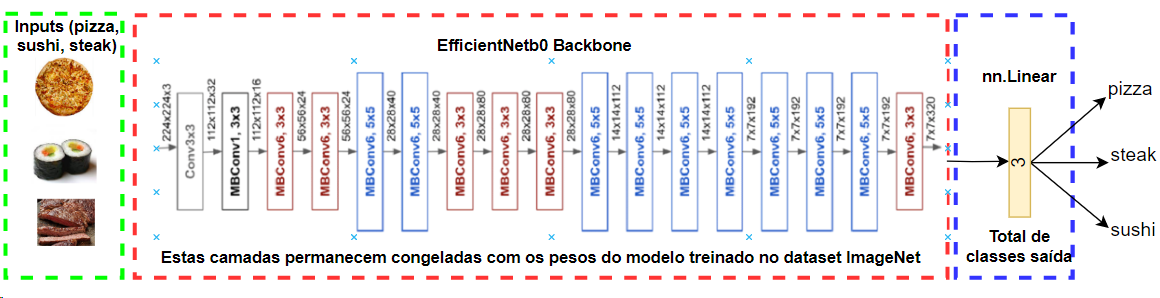
\includegraphics[width=1\linewidth]{figures/transfer_learning01}
	\end{figure}
		
	\end{block}
\end{frame} 

%==========================================================================================
\begin{frame}
	\frametitle{PyTorch Transfer Learning}
	\begin{block}{PyTorch Transfer Learning}
		Os passos que vamos fazer:
		\begin{itemize}
			\item[5] Vamos trocar a saída da última camada da EfficientNetb0 de 1000 (ImageNet) para 3 (FoodVision) e deixar as demais camadas congeladas
			\item[5] Treinar o modelo
			\item[6] Avaliar o modelo
			\item[7] Realizar predição com o modelo no conjunto de teste
			\item[8] Fazendo previsões em uma imagem personalizada
		\end{itemize}
	\end{block}
\end{frame} 

%==========================================================================================
\section{PyTorch Paper Replicating}



\begin{frame}
	\frametitle{PyTorch - Paper Replicating}
	\begin{block}{Machine Learning Research paper}
		\begin{table}[]
			\resizebox{\textwidth}{!}{%
				\begin{tabular}{|l|l|}
					\hline
					\textbf{Seção} & \textbf{Objetivo}                          \\ \hline
					Resumo     & \begin{tabular}[c]{@{}l@{}}Overview/summary do artigo contendo\\ principais achados/contribuições.\end{tabular}                    \\ \hline
					Introdução & \begin{tabular}[c]{@{}l@{}}Qual o problema a ser explorado.\\ Métodos antecessores usados neste problema.\end{tabular}             \\ \hline
					Métodos    & \begin{tabular}[c]{@{}l@{}}Passos para que pesquisadores possam\\ conduzir sua pesquisa (Datasource, trainning, etc).\end{tabular} \\ \hline
					Resultados & \begin{tabular}[c]{@{}l@{}}Resultado do paper. Uma comparação\\ com resultados de outras pesquisas.\end{tabular}                   \\ \hline
					Conclusões     & Conclusões, limitações e trabalhos futuros \\ \hline
					Referências    & Fontes/outras pesquisas                    \\ \hline
					Apendices      & Recursos extras                            \\ \hline
				\end{tabular}%
			}
		\end{table}
	\end{block}
\end{frame}  
%==========================================================================================
\begin{frame}
	\frametitle{PyTorch - Paper Replicating}
	\begin{block}{Machine Learning Research paper}
	\begin{figure}
		\centering
		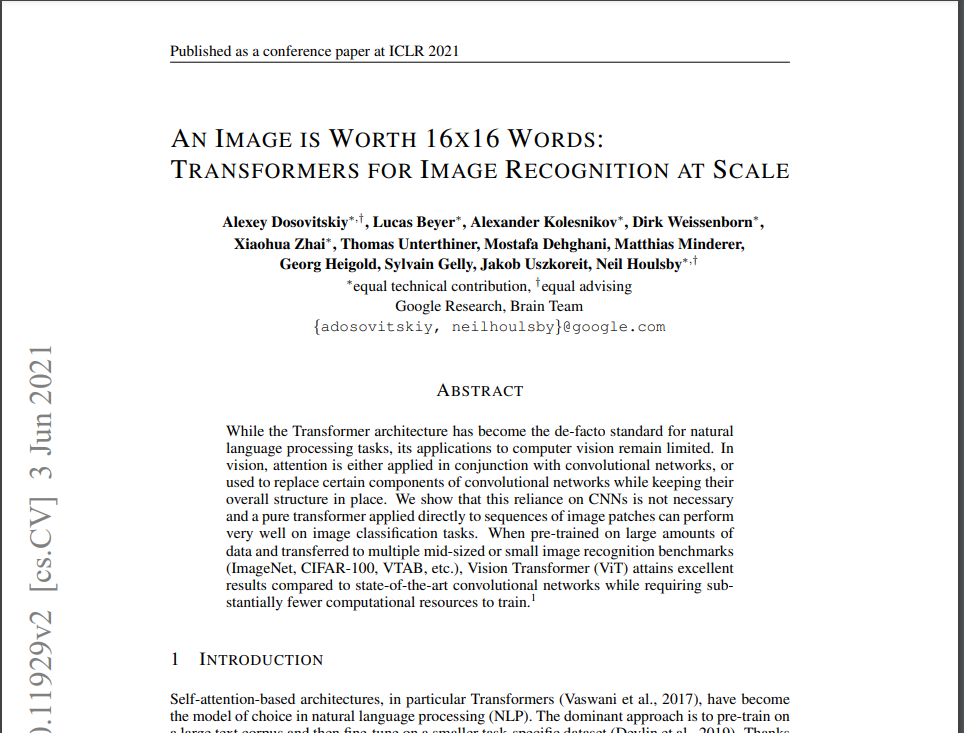
\includegraphics[width=0.7\linewidth]{figures/an-image-is-worth-16x16-words-transformers-1}
	\end{figure}
	\end{block}
\end{frame} 
%==========================================================================================
\begin{frame}
	\frametitle{PyTorch - Paper Replicating}
	\begin{block}{Por que replicar um artigo}
		\begin{itemize}
			\item Porque é divertido e desafiador!
			\item Os avanços da ciência são registrados em artigos, podemos aplicá-los aos nossos problemas.
		\end{itemize}
	\end{block}
	\begin{block}{Por que replicar um artigo}
		George Hotz. fundador da comma.ai
		\begin{itemize}
			\item Baixe o artigo
			\item Replique ele
			\item Continue fazendo até você ter mais habilidades/skills
		\end{itemize}
	\end{block}
\end{frame} 
%==========================================================================================
\begin{frame}
	\frametitle{PyTorch - Paper Replicating}
	\begin{block}{Vision Transform}
		Transformer architecture é qualquer rede que utiliza mecanismos de atenção. Similar às redes CNN que usam convolução nas camadas iniciais. Vamos fazer:
		\begin{itemize}
			\item[1] Configurar o ambiente e projeto
			\item[2] Obter dados
			\item[3] Criar conjunto de dados e carregar nos Dataloaders
			\item[4] Replicar o artigo ViT: uma visão geral
			\item[5] Equação 1: a incorporação do patch
			\item[6] Equação 2: Atenção Multihead (MSA)
			\item[7] Equação 3: Multilayer Perceptron (MLP)
		\end{itemize}
	\end{block}
\end{frame} 
%==========================================================================================
\begin{frame}
	\frametitle{PyTorch - Paper Replicating}
	\begin{block}{Vision Transform}
		Transformer architecture é qualquer rede que utiliza mecanismos de atenção. Similar às redes CNN que usam convolução nas camadas iniciais. Vamos fazer:
		\begin{itemize}
			\item[8] Criar o Transformer Encode
			\item[9] Juntar tudo para criar o ViT
			\item[10] Configurar o código de treinamento para nosso modelo ViT
			\item[11] Usar um ViT pré-treinado de torchvision.models
			\item[12] Fazer previsões em uma imagem personalizada
		\end{itemize}
	\end{block}
\end{frame} 
%==========================================================================================

%==========================================================================================
\begin{frame}
	\frametitle{PyTorch - Paper Replicating}
	\begin{block}{Vision Transform - Configurar o ambiente e projeto}
		\begin{itemize}
			\item Escrevemos bastante código útil nas últimas seções, vamos baixá-lo e garantir que possamos usá-lo novamente.
			\item Vamos importar nossos scripts modular.
			\item Vamos importar algumas funções helper\_functions.py
			\item Utilize a GPU modificando nas configurações do Colab
		\end{itemize}
	\end{block}
	\begin{alertblock}{Nota}
		Sempre reinicie o ambiente do colab ao fazer novas instalações
	\end{alertblock}
\end{frame}
%==========================================================================================
\begin{frame}
	\frametitle{PyTorch - Paper Replicating}
	\begin{block}{Vision Transform - Obter dados}
		\begin{itemize}
			\item Baixe o dataset usando a função download\_data() do helper\_functions.py
			\item Crie os caminhos de diretórios de train e test
		\end{itemize}
	\end{block}
	\begin{block}{Vision Transform - Criar conjunto de dados e carregar nos Dataloaders}
		\begin{itemize}
			\item Carregar as imagens
			\item Preparar transforms para images
			\item Carregar images no DataLoader
			\item Visualizar uma imagem
		\end{itemize}
	\end{block}
\end{frame} 
%==========================================================================================
\begin{frame}
	\frametitle{PyTorch - Paper Replicating}
	\begin{block}{Vision Transform - Uma visão geral}
		\begin{itemize}
			\item Como é formada uma Rede neural: Camadas, Blocos e modelo.
			\item Como o ViT paper foi feito: Figura 1, Formulas e Tabelas.
		\end{itemize}
	\end{block}
	\begin{block}{Figura 1}
		\begin{figure}
			\centering
			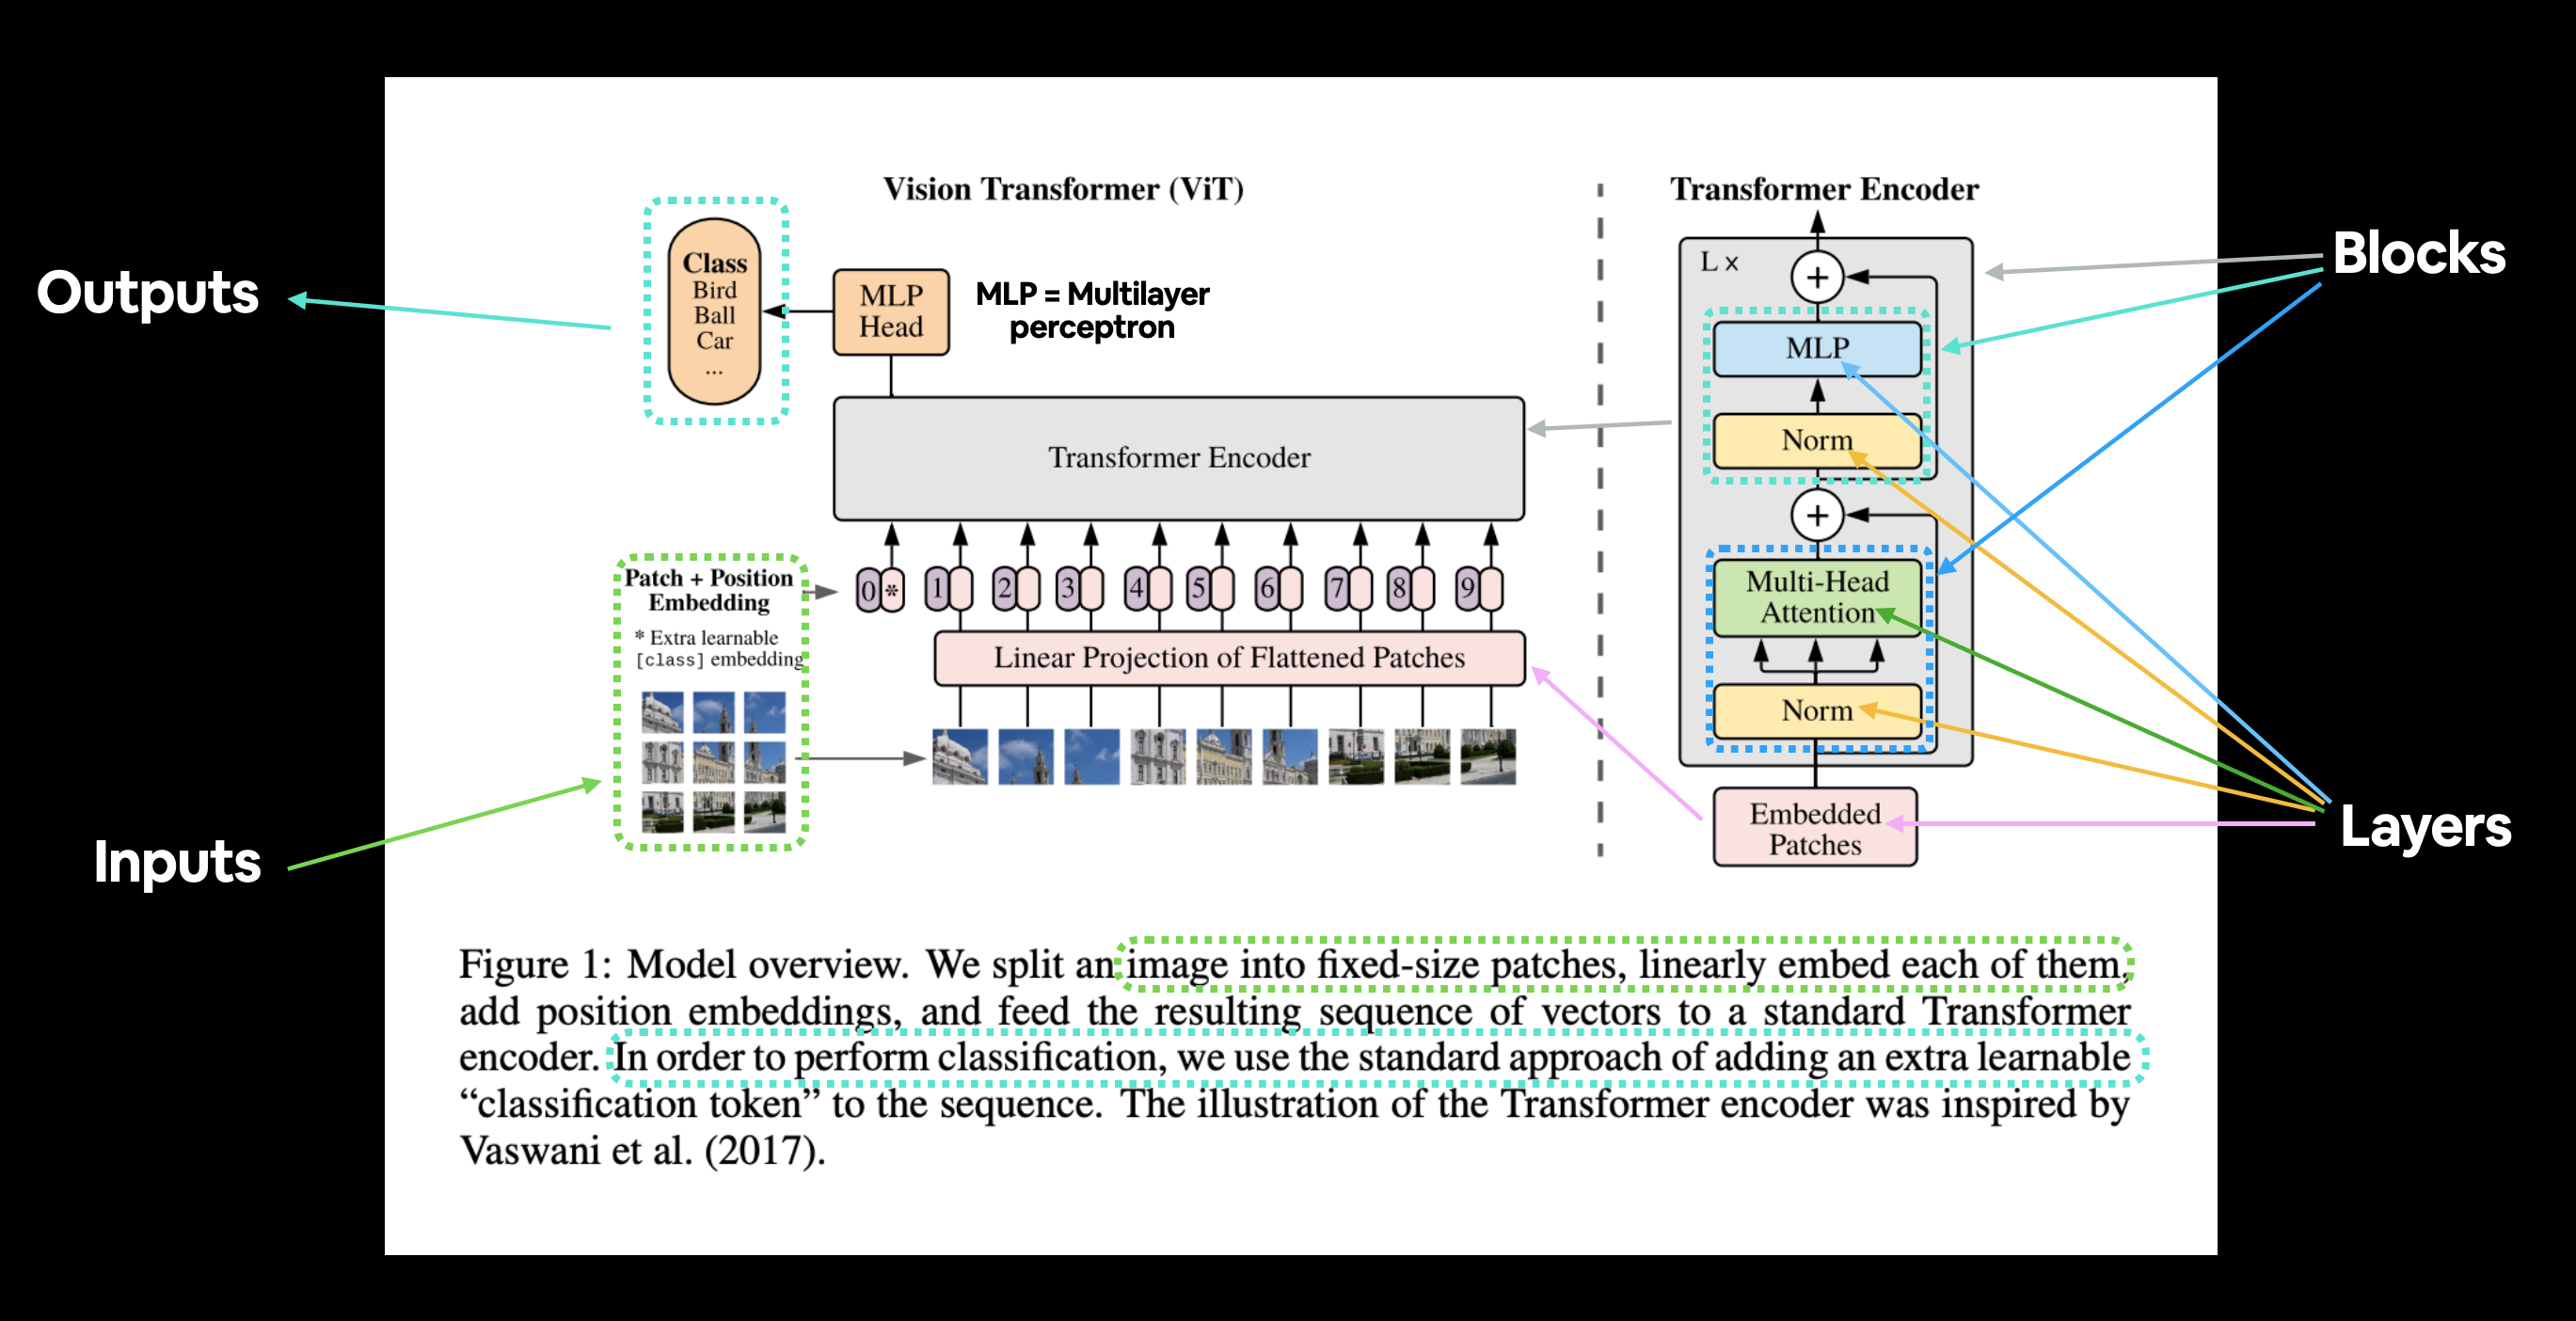
\includegraphics[width=0.7\linewidth]{figures/vit_fig_1}
		\end{figure}
	
	\end{block}
\end{frame} 
%==========================================================================================
\begin{frame}
	\frametitle{PyTorch - Paper Replicating}
	\begin{block}{Vision Transform - Uma visão geral}
		A arquitetura ViT é composta por várias etapas:
		\begin{itemize}
			\item \textbf{Patch + Position Embedding (inputs)} - Transforma a imagem de entrada em uma sequência de patches de imagem e adiciona um número de posição na ordem em que o patch vem.
			\item \textbf{Linear projection of flattened patches (Embedded Patches)} - Os patches de imagem são transformados em uma incorporação, o benefício de usar uma incorporação em vez de apenas os valores da imagem é que uma incorporação é uma representação aprendizável (normalmente na forma de um vetor) da imagem que pode melhorar com o treinamento.
			\item \textbf{Norm} - É a abreviação de "Layer Normalization" ou "LayerNorm", uma técnica para regularizar (reduzir o overfitting) uma rede neural, você pode usar LayerNorm através da camada PyTorch torch.nn.LayerNorm().
		\end{itemize}
	\end{block}
\end{frame}
%==========================================================================================
\begin{frame}
	\frametitle{PyTorch - Paper Replicating}
	\begin{block}{Vision Transform - Uma visão geral}
		A arquitetura ViT é composta por várias etapas:
		\begin{itemize}
			\item \textbf{Multi-Head Attention} - Esta é uma camada de auto-atenção com várias heads ou "MSA" para abreviar. Você pode criar uma camada MSA por meio da camada PyTorch torch.nn.MultiheadAttention().
			\item \textbf{MLP (ou Multilayer perceptron)} - Um MLP geralmente pode se referir a qualquer coleção de camadas de feedforward (ou no caso do PyTorch, uma coleção de camadas com um método forward()). No ViT Paper, os autores referem-se ao MLP como "bloco MLP" e contém dois torch.nn.Linear() com uma ativação não linear torch.nn.GELU() entre elas (seção 3.1) e uma camada torch.nn.Dropout() após cada (Apêndice B.1).
		\end{itemize}
	\end{block}
\end{frame}
%==========================================================================================
\begin{frame}
	\frametitle{PyTorch - Paper Replicating}
	\begin{block}{Vision Transform - Uma visão geral}
		A arquitetura ViT é composta por várias etapas:
		\begin{itemize}
			\item \textbf{Transformer Encoder} - O Transformer Encoder é uma coleção das camadas listadas acima. Existem duas conexões de salto dentro do codificador Transformer (os símbolos "+"), o que significa que as entradas da camada são alimentadas diretamente para as camadas imediatas, bem como para as camadas subsequentes. A arquitetura geral do ViT é composta por vários codificadores Transformer empilhados uns sobre os outros.
			\item \textbf{MLP Head} - Esta é a camada de saída da arquitetura, ela converte os recursos aprendidos de uma entrada em uma saída de classe. Como estamos trabalhando na classificação de imagens, você também pode chamar isso de "cabeça do classificador". A estrutura do cabeçote MLP é semelhante ao bloco MLP.
		\end{itemize}
	\end{block}
\end{frame}
%==========================================================================================
\begin{frame}
	\frametitle{PyTorch - Paper Replicating}
	\begin{block}{Vision Transform - Explorando as quatro equações}
		$\begin{aligned} \mathbf{z}_0 & =\left[\mathbf{x}_{\text {class }} ; \mathbf{x}_p^1 \mathbf{E} ; \mathbf{x}_p^2 \mathbf{E} ; \cdots ; \mathbf{x}_p^N \mathbf{E}\right]+\mathbf{E}_{\text {pos }}, & & \mathbf{E} \in \mathbb{R}^{\left(P^2 \cdot C\right) \times D}, \mathbf{E}_{\text {pos }} \in \mathbb{R}^{(N+1) \times D} \\ \mathbf{z}_{\ell}^{\prime} & =\operatorname{MSA}\left(\mathrm{LN}\left(\mathbf{z}_{\ell-1}\right)\right)+\mathbf{z}_{\ell-1}, & & \ell=1 \ldots L \\ \mathbf{z}_{\ell} & =\operatorname{MLP}\left(\operatorname{LN}\left(\mathbf{z}_{\ell}^{\prime}\right)\right)+\mathbf{z}_{\ell}^{\prime}, & & \ell=1 \ldots L \\ \mathbf{y} & =\operatorname{LN}\left(\mathbf{z}_L^0\right) & & \end{aligned}$
	\end{block}
\end{frame}
%==========================================================================================
\begin{frame}
	\frametitle{PyTorch - Paper Replicating}
	\begin{block}{Vision Transform - Explorando as quatro equações}
		\begin{itemize}
			\item[Eq.1] O Transformer usa tamanho de vetor latente constante D em todas as suas camadas, então achatamos (flatten) os patches e mapeamos para as dimensões D com uma \textbf{projeção linear treinável} (Eq. 1). Referimo-nos à saída desta projeção como os \textbf{embeddings de patch}... Embeddings de posição são adicionados aos embeddings de patch para reter informações posicionais. Usamos incorporações de posição 1D aprendíveis padrão.
			\item[Eq.2] O codificador Transformer (Vaswani et al., 2017) consiste em camadas alternadas de multihead self-attention (MSA, consulte o Apêndice A) e blocos MLP (Eq. 2, 3). Layernorm (LN) é aplicado antes de cada bloco e conexões residuais após cada bloco (Wang et al., 2019; Baevski \& Auli, 2019).
		\end{itemize}
	\end{block}
\end{frame}
%==========================================================================================
\begin{frame}
	\frametitle{PyTorch - Paper Replicating}
	\begin{block}{Vision Transform - Explorando as quatro equações}
		\begin{itemize}
			\item[Eq.3] Idem Eq.2
			\item[Eq.4] Semelhante ao token [class] do BERT, anexamos learnable embedding que pode ser aprendida à sequência de embedded patches (z00=xclass), cujo estado na saída do codificador Transformer (z0L) serve como a representação da imagem y (Eq. 4).
		\end{itemize}
	\end{block}
\end{frame}
%==========================================================================================
\begin{frame}
	\frametitle{PyTorch - Paper Replicating}
	\begin{block}{Vision Transform - Explorando as quatro equações}
		\begin{figure}
			\centering
			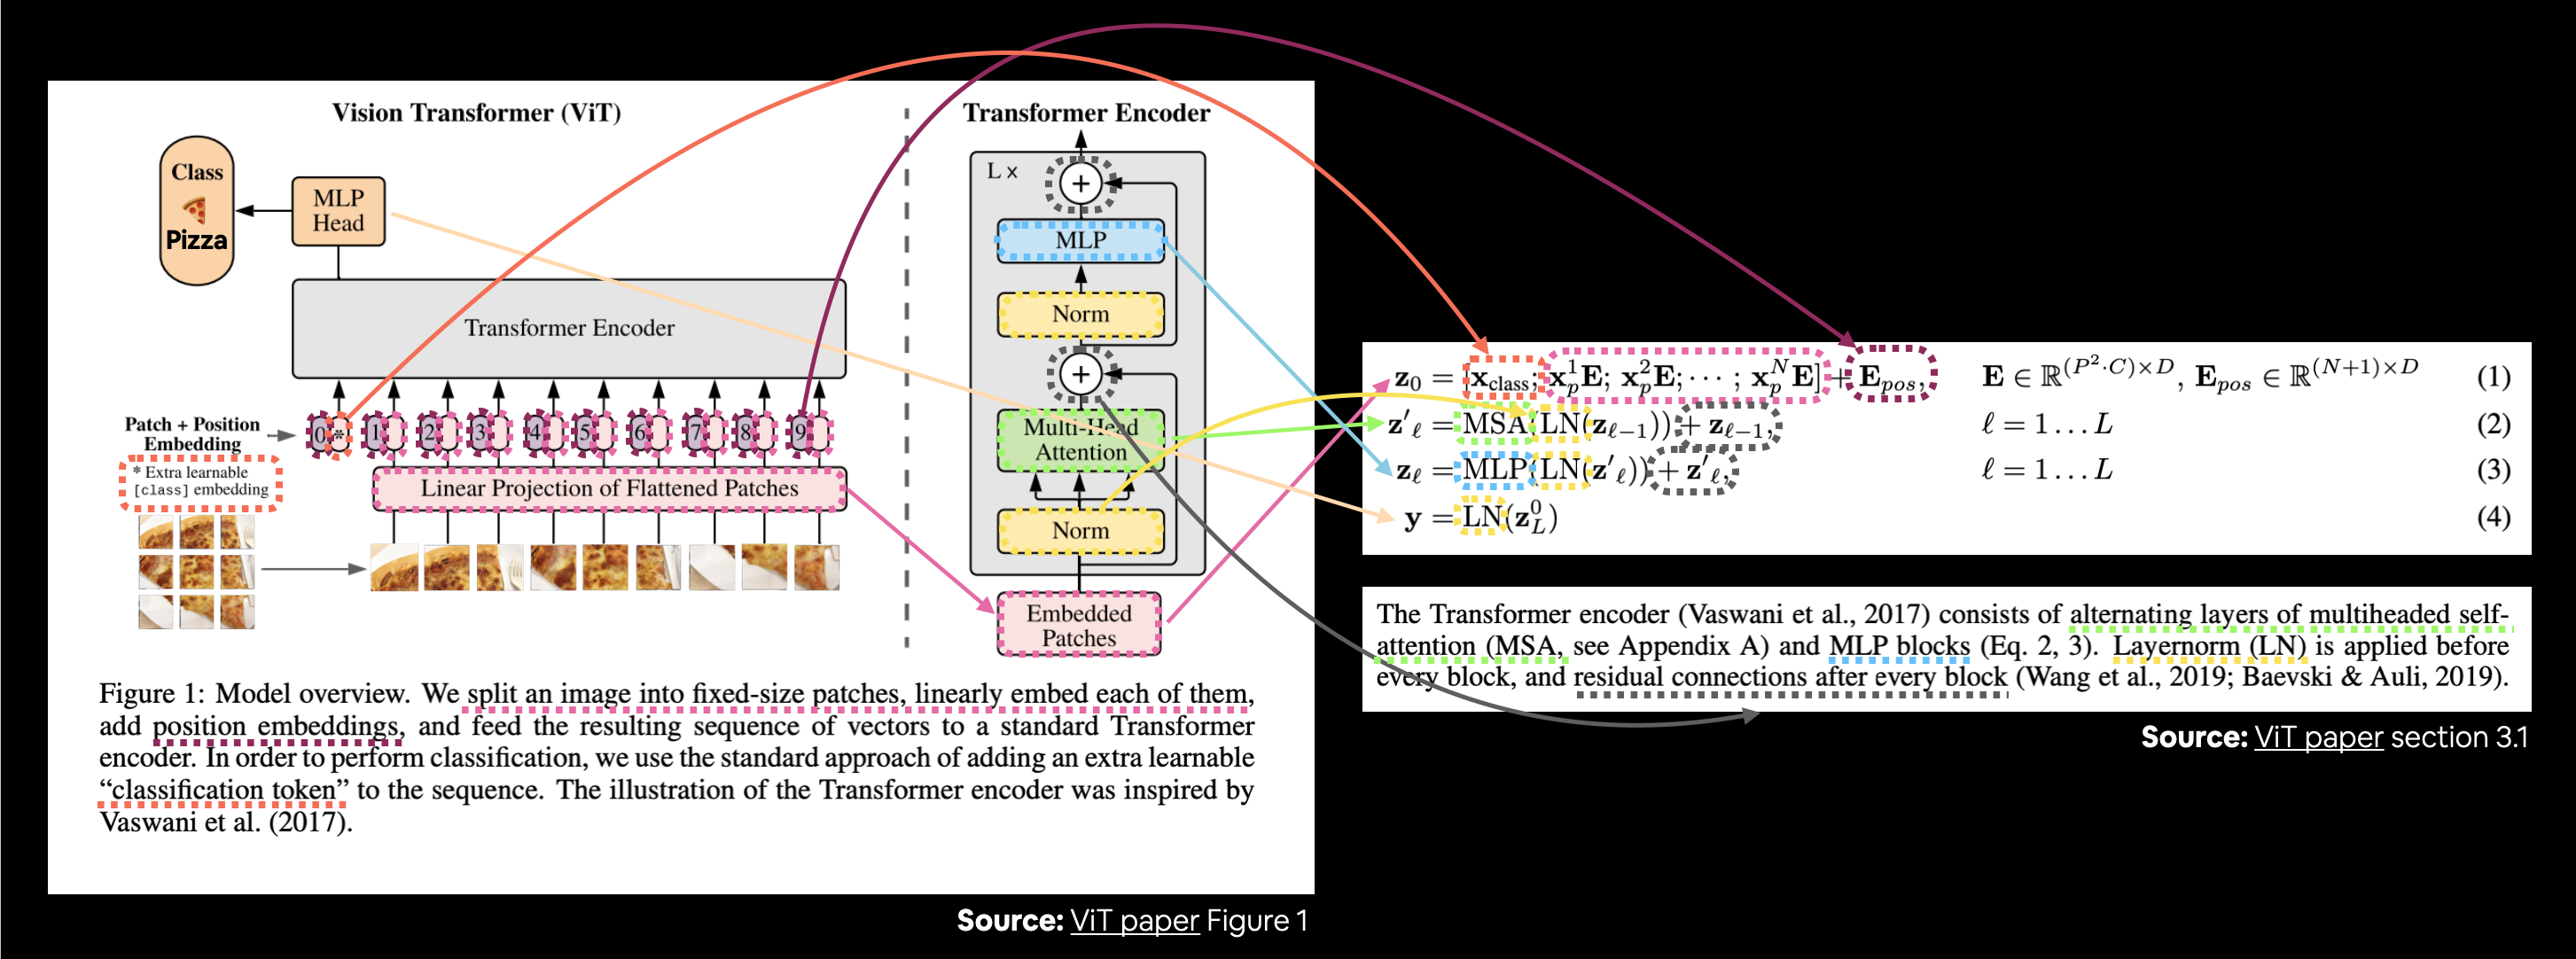
\includegraphics[width=1\linewidth]{figures/vit_fig1_eqs}
		\end{figure}
		\begin{itemize}
			\item \textbf{z0}  is "z zero" (this is the output of the initial patch embedding layer).
			\item \textbf{z´l } is "z of a particular layer prime" (or an intermediary value of z).
			\item \textbf{zl}  is "z of a particular layer".
			\item \textbf{y} is output
		\end{itemize}
	\end{block}
\end{frame}
%==========================================================================================
\begin{frame}
	\frametitle{PyTorch - Paper Replicating}
	\begin{block}{Vision Transform - Equação 01}
		$$
		\begin{aligned}
			\mathbf{z}_{0} &=\left[\mathbf{x}_{\text {class }} ; \mathbf{x}_{p}^{1} \mathbf{E} ; \mathbf{x}_{p}^{2} \mathbf{E} ; \cdots ; \mathbf{x}_{p}^{N} \mathbf{E}\right]+\mathbf{E}_{\text {pos }}, & & \mathbf{E} \in \mathbb{R}^{\left(P^{2} \cdot C\right) \times D}, \mathbf{E}_{\text {pos }} \in \mathbb{R}^{(N+1) \times D}
		\end{aligned}
		$$
		Esta equação trata do token de classe, incorporação de patch e incorporação de posição ($\mathbf{E}$ é para incorporação) da imagem de entrada. \\
		x\_input = [class\_token, image\_patch\_1, image\_patch\_2, image\_patch\_3...] + [class\_token\_position, image\_patch\_1\_position, image\_patch\_2\_position, image\_patch\_3\_position...] \\
		Onde cada um dos elementos no vetor pode ser aprendido (seus requires\_grad=True).
	\end{block}
\end{frame}
%==========================================================================================
\begin{frame}
	\frametitle{PyTorch - Paper Replicating}
	\begin{block}{Vision Transform - Equação 02}
		$$
		\begin{aligned}
			\mathbf{z}_{\ell}^{\prime} &=\operatorname{MSA}\left(\operatorname{LN}\left(\mathbf{z}_{\ell-1}\right)\right)+\mathbf{z}_{\ell-1}, & & \ell=1 \ldots L
		\end{aligned}
		$$

		Isso diz que para cada camada de $1$ até $L$ (o número total de camadas), há uma camada Multi-Head Attention (MSA) envolvendo uma camada LayerNorm (LN). \\
		A adição no final é o equivalente a adicionar a entrada à saída e formar um skip/residual connection \href{https://paperswithcode.com/method/residual-connection}{\beamergotobutton{skip/residual connection}} \\
		Chamaremos essa camada de "bloco MSA". \\
		
		x\_output\_MSA\_block = MSA\_layer(LN\_layer(x\_input)) + x\_input \\ 
		Observe a conexão de salto no final (adicionando a entrada das camadas à saída das camadas).
	\end{block}
\end{frame}
%==========================================================================================
\begin{frame}
	\frametitle{PyTorch - Paper Replicating}
	\begin{block}{Vision Transform - Equação 03}
		$$
		\begin{aligned}
			\mathbf{z}_{\ell} &=\operatorname{MLP}\left(\operatorname{LN}\left(\mathbf{z}_{\ell}^{\prime}\right)\right)+\mathbf{z}_{\ell}^{\prime}, & & \ell=1 \ldots L \\
		\end{aligned}
		$$
		
		
		Isso diz que para cada camada de $1$ até $L$ (o número total de camadas), há também uma camada Multilayer Perceptron (MLP) envolvendo uma camada LayerNorm (LN).
		
		A adição no final mostra a presença de uma conexão de salto/residual.
		
		Chamaremos essa camada de "bloco MLP". 
		
		x\_output\_MLP\_block = MLP\_layer(LN\_layer(x\_output\_MSA\_block)) + x\_output\_MSA\_block
		\\ Observe a conexão de salto no final (adicionando a entrada das camadas à saída das camadas).
	\end{block}
\end{frame}
%==========================================================================================
\begin{frame}
	\frametitle{PyTorch - Paper Replicating}
	\begin{block}{Vision Transform - Equação 04}
		$$
		\begin{aligned}
			\mathbf{y} &=\operatorname{LN}\left(\mathbf{z}_{L}^{0}\right) & &
		\end{aligned}
		$$
		
		Isso diz que para a última camada $L$, a saída $y$ é o token de índice 0 de $z$ envolvido em uma camada LayerNorm (LN).
		
		Ou no nosso caso, o índice 0 de `x\_output\_MLP\_block`: \\
		y = Linear\_layer(LN\_layer(x\_output\_MLP\_block[0]))
	\end{block}
\end{frame}
%==========================================================================================
\begin{frame}
	\frametitle{PyTorch - Paper Replicating}
	\begin{block}{Vision Transform - Tabela 01}
		\begin{table}[!ht]
			\centering
			\begin{tabular}{|l|l|l|l|l|l|}
				\hline
				Model & Layers & Hidden size $D$ & MLP size & Heads & Params \\ \hline
				ViT-Base & 12 & 768 & 3072 & 12 & $86M$ \\ \hline
				ViT-Large & 24 & 1024 & 4096 & 16 & $307M$ \\ \hline
				ViT-Huge & 32 & 1280 & 5120 & 16 & $632M$ \\ \hline
			\end{tabular}
		\end{table}
		\begin{itemize}
			\item \textbf{Camadas} - Quantos blocos do Transformer Encoder existem? (cada um deles conterá um bloco MSA e um bloco MLP)
			\item \textbf{Hidden size  D } - Esta é a dimensão de incorporação em toda a arquitetura, este será o tamanho do vetor em que nossa imagem se transforma quando é corrigida e incorporada. Geralmente, quanto maior a dimensão de incorporação, mais informações podem ser capturadas, melhores resultados. No entanto, uma incorporação maior tem o custo de mais computação.
		\end{itemize}
	\end{block}
\end{frame}
%==========================================================================================
\begin{frame}
	\frametitle{PyTorch - Paper Replicating}
	\begin{block}{Vision Transform - Tabela 01}
		\begin{table}[!ht]
			\centering
			\begin{tabular}{|l|l|l|l|l|l|}
				\hline
				Model & Layers & Hidden size $D$ & MLP size & Heads & Params \\ \hline
				ViT-Base & 12 & 768 & 3072 & 12 & $86M$ \\ \hline
				ViT-Large & 24 & 1024 & 4096 & 16 & $307M$ \\ \hline
				ViT-Huge & 32 & 1280 & 5120 & 16 & $632M$ \\ \hline
			\end{tabular}
		\end{table}
		\begin{itemize}
			\item \textbf{Heads} - Quantas cabeças existem nas camadas Multi-Head Attention?
			\item \textbf{Params} - Qual é o número total de parâmetros do modelo? Geralmente, mais parâmetros levam a um melhor desempenho, mas ao custo de mais computação. Você notará que até o ViT-Base tem muito mais parâmetros do que qualquer outro modelo que usamos até agora.
		\end{itemize}
	\end{block}
\end{frame}
%==========================================================================================
\begin{frame}
	\frametitle{PyTorch - Paper Replicating}
	\begin{block}{Vision Transform - Passos para replicação}
		\begin{itemize}
			\item 1. Leia todo o artigo de ponta a ponta uma vez (para ter uma ideia dos principais conceitos).
			\item 2. Volte a cada seção e veja como elas se alinham e comece a pensar em como elas podem ser transformadas em código (como acima).
			\item 3. Repita a etapa 2 até obter um esboço razoavelmente bom.
			\item 4. Use mathpix.com(https://mathpix.com/) (uma ferramenta muito útil) para transformar todas as seções do papel em markdown/LaTeX para colocar em textos.
			\item 5. Replique a versão mais simples possível do modelo.
			\item 6. Se ficar preso, procure outros exemplos.
		\end{itemize}
	\end{block}
\end{frame}
%==========================================================================================
\begin{frame}
	\frametitle{PyTorch - Paper Replicating}
	\begin{block}{Vision Transform - Passos para replicação}
		\begin{itemize}
			\item 1. Leia todo o artigo de ponta a ponta uma vez (para ter uma ideia dos principais conceitos).
			\item 2. Volte a cada seção e veja como elas se alinham e comece a pensar em como elas podem ser transformadas em código (como acima).
			\item 3. Repita a etapa 2 até obter um esboço razoavelmente bom.
			\item 4. Use mathpix.com(https://mathpix.com/) (uma ferramenta muito útil) para transformar todas as seções do papel em markdown/LaTeX para colocar em textos.
			\item 5. Replique a versão mais simples possível do modelo.
			\item 6. Se ficar preso, procure outros exemplos.
		\end{itemize}
	\end{block}
\end{frame}
%==========================================================================================
\begin{frame}
	\frametitle{PyTorch - Paper Replicating}
	\begin{block}{Vision Transform - Vamos replicar a equação 01}
		Se você puder representar seus dados de uma maneira boa e aprendível (já que as incorporações são representações aprendíveis), é provável que um algoritmo de aprendizado seja capaz de ter um bom desempenho com eles. Vamos começar com \textbf{\textbf{patch embedding}}: 
		A entrada do tramsform é de 1D de token embeddings. Para imagens 2D, remodelamos a imagem $\mathbf{x} \in \mathbb{R}^{H \times W \times C}$ em uma sequência de patches 2D achatados (flatten) $\mathbf{x}_{p} \in \mathbb{R}^{N \times\left(P^{2} \cdot C\right)}$, onde $(H, W)$ é a resolução da imagem original, $C$ é o número de canais, $(P, P)$ é a resolução de cada patch de imagem e $N=H W / P^{2}$ é o número resultante de patches, que também serve como o comprimento efetivo da sequência de entrada para o Transformer. O Transformer usa tamanho de vetor latente constante $D$ em todas as suas camadas, portanto achatamos os patches e mapeamos para as dimensões $D$ com uma projeção linear treinável (Eq. 1). Referimo-nos à saída dessa projeção \textbf{como embeddings de patch}.
	\end{block}
\end{frame}
%==========================================================================================
\begin{frame}
	\frametitle{PyTorch - Paper Replicating}
	\begin{block}{Vision Transform - Vamos replicar a equação 01}
		\begin{itemize}
			\item Training resolution is $224$.
			\item $D$  is the size of the patch embeddings
			\item The image starts as $2D$ with size  $H×W×C$.
			\item The image gets converted to a sequence of flattened 2D patches with size ${N \times\left(P^{2} \cdot C\right)}$.
			\begin{itemize}
				\item $(P, P)$ is the resolution of each image patch (patch size).
				\item $N=H W / P^{2}$ is the resulting number of patches, which also serves as the input sequence length for the Transformer.
			\end{itemize}
			
		\end{itemize}
	\end{block}
\end{frame}
%==========================================================================================
\begin{frame}
	\frametitle{PyTorch - Paper Replicating}
	\begin{block}{Vision Transform - Vamos replicar a equação 01}
		\begin{figure}
			\centering
			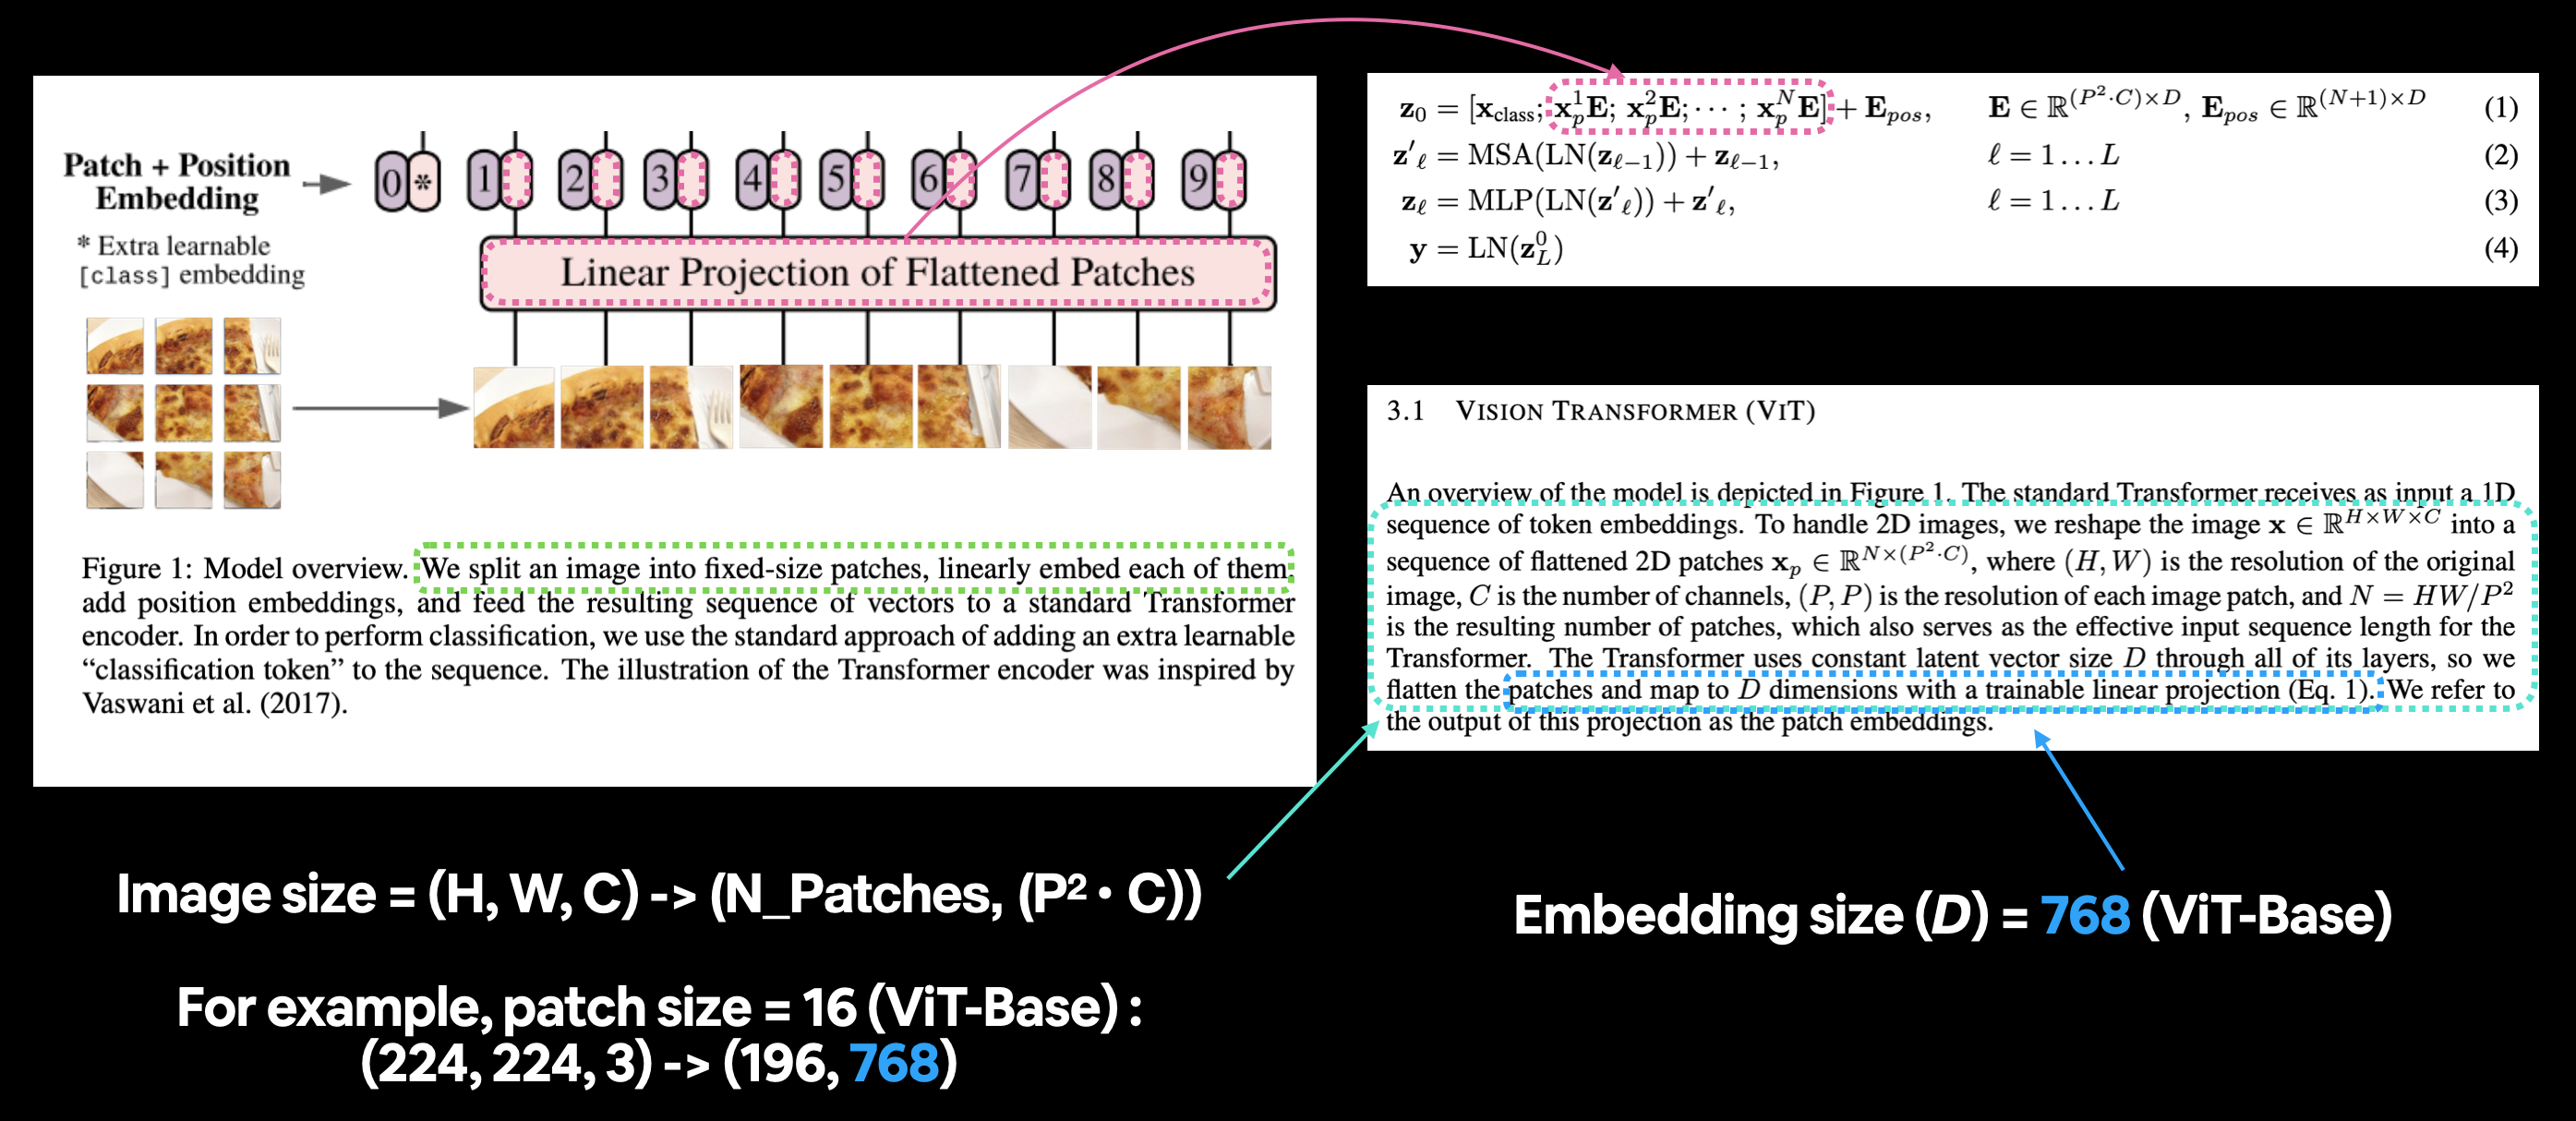
\includegraphics[width=1\linewidth]{figures/vit_fig1_eqs1}
		\end{figure}
	Vamos calcular os shapes de entrada e saída de patch embedding manualmente. Vamos deicar o valor de \textbf{P} = 16 ``ViT-B/16''.
	\end{block}
	
\end{frame}
%==========================================================================================
\begin{frame}
	\frametitle{PyTorch - Paper Replicating}
	\begin{block}{Vision Transform - Vamos replicar a equação 01}
		Assim teremos: \\
		- \textbf{input:} Imagens que começa como 2D com tamanho  ${H \times W \times C}$
		- \textbf{Output:} A imagem convertida em uma sequencia achatada com tamanho ${N \times\left(P^{2} \cdot C\right)}$
		\begin{figure}
			\centering
			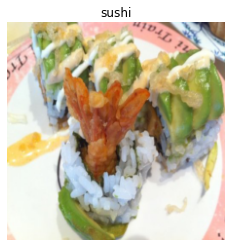
\includegraphics[width=0.4\linewidth]{figures/vit_patch_ex00}
		\end{figure}
		
	\end{block}
	
\end{frame}
%==========================================================================================
\begin{frame}
	\frametitle{PyTorch - Paper Replicating}
	\begin{block}{Vamos replicar a equação 01 - Transformando uma única imagem em patches}
		Transformando uma única imagem em patches: \\
		Agora que conhecemos as formas ideais de entrada e saída para nossa camada patch embedding, vamos prosseguir para criá-la. \\
		Vamos vizualizar nossa imagem em patch
		\begin{figure}
			\centering
			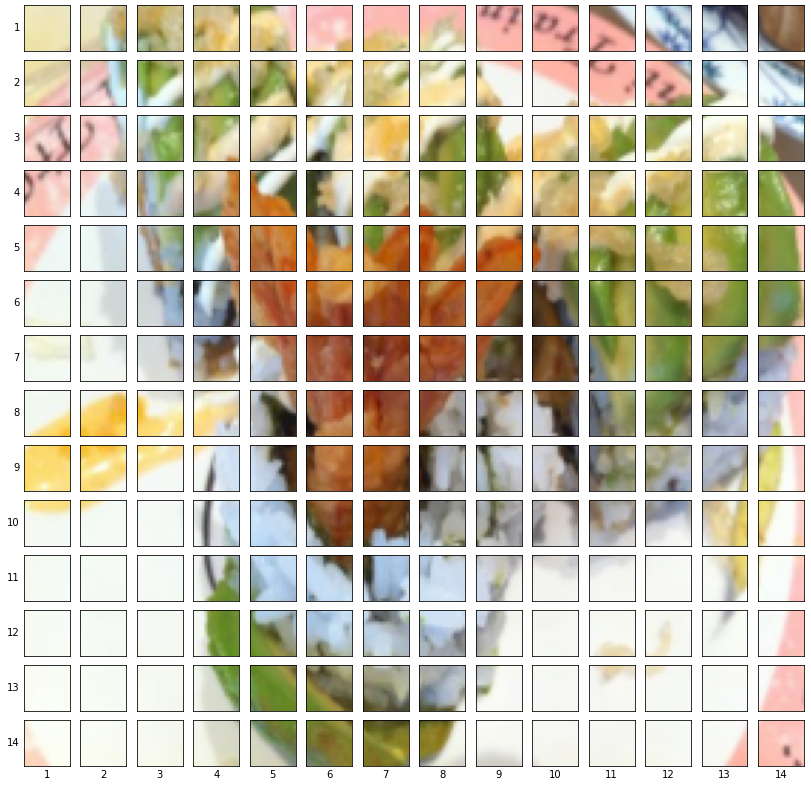
\includegraphics[width=0.4\linewidth]{figures/vit_patch_ex01}
		\end{figure}
	\end{block}
\end{frame}
%==========================================================================================
\begin{frame}
	\frametitle{PyTorch - Paper Replicating}
	\begin{block}{Vamos replicar a equação 01 - Criando patches de imagem com torch.nn.Conv2d()}
		\textbf{Hybrid Architecture: }Como uma alternativa aos patches de imagens brutas, a sequência de entrada pode ser formada a partir de mapas de recursos de uma CNN (LeCun et al., 1989). Neste modelo híbrido, a projeção de patch embedding \textbf{E } (Eq. 1) é aplicada a patches extraídos de um mapa de features CNN. Como um caso especial, os patches podem ter tamanho espacial  1×1 , o que significa que a sequência de entrada é obtida simplesmente achatando as dimensões espaciais do mapa de features e projetando para a dimensão do Transformer. \\
		O \textbf{``mapa de features''} a que eles se referem são os pesos/ativações produzidos por uma camada convolucional que passa sobre uma determinada imagem. \\
		\href{https://github.com/mafaldasalomao/pavic_treinamento_ml/blob/main/Machine_Learning/figures/08-vit-paper-patch-embedding-animation.gif?raw=true}{\beamergotobutton{Acessar}} 
	\end{block}
\end{frame}
%==========================================================================================
\begin{frame}
	\frametitle{PyTorch - Paper Replicating}
	\begin{block}{Vamos replicar a equação 01 - Criando patches de imagem com torch.nn.Conv2d()}
		Com os parâmetros \textbf{kernel\_size} e \textbf{stride} de uma camada \textbf{torch.nn.Conv2d()} iguais ao \textbf{patch\_size} podemos efetivamente obter uma camada que divide nossa imagem em patches e cria uma incorporação que pode ser aprendida (conhecida como "Linear Projection" no artigo do ViT) de cada patch.
	\end{block}
	\begin{block}{O que vamos fazer}
		Usaremos: \textbf{torch.nn.Conv2d()} para transformar nossa imagem em patches de mapas de features da CNN. E, \textbf{torch.nn.Flatten()} para achatar as dimensões espaciais do mapa de features. 
		O kernel size  = 16 = patch size e stride = 16 = patch size, ou seja, filtragem do tamanho do patch e pular 16 pixels para realizar nova filtragem. \\
		in\_channels=3 e out\_channels=768 vindo da nossa fórmula anterior $D$
		
	\end{block}
\end{frame}
%==========================================================================================
\begin{frame}
	\frametitle{PyTorch - Paper Replicating}
	\begin{block}{Vamos replicar a equação 01 - Criando patches de imagem com torch.nn.Conv2d()}
		Vamos passar uma imagem pela camada recém criada e analisar sua saída:
		\begin{figure}
			\centering
			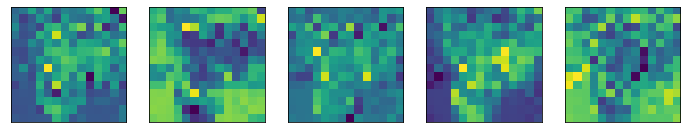
\includegraphics[width=0.7\linewidth]{figures/vit_patch_cnn_out01}
		\end{figure}
		
		Observe como todos os mapas de recursos representam a imagem original, depois de visualizar mais alguns, você pode começar a ver os diferentes contornos principais e alguns recursos principais.
		
		O importante a observar é que esses recursos podem mudar com o tempo à medida que a rede neural aprende.
		
		E por causa disso, esses mapas de recursos podem ser considerados uma \textbf{incorporação que pode ser aprendida} da nossa imagem.

	\end{block}
\end{frame}
%==========================================================================================




\begin{frame}
	\frametitle{PyTorch - Paper Replicating}
	\begin{block}{Vamos replicar a equação 01 - Achatando a incorporação do patch com torch.nn.Flatten()}
		Transformamos nossa imagem em incorporações de patch, mas elas ainda estão no formato 2D. \\
		Como os colocamos na forma de saída desejada da camada de incorporação de patch do modelo ViT? \\
		Saída desejada (1D sequence of flattened 2D patches): (196, 768) $\rightarrow$ (number of patches, embedding dimension) $\rightarrow$ ${N \times\left(P^{2} \cdot C\right)}$ \\
		Temos a saída com 768 partes  ( $(P^{2} \cdot C)$ ), mas precisamos do número de patches $N$.
		
		\alert{Os patches podem ter tamanho de $1 \times 1$ o que significa que para obtê-lo basta \textbf{achatarmos o mapa de fature} e projetá-lo para o Transformer}
		
		
	\end{block}
\end{frame}

%==========================================================================================
\begin{frame}
	\frametitle{PyTorch - Paper Replicating}
	\begin{block}{Vamos replicar a equação 01 -Transformando a patch embedding layer ViT em um módulo PyTorch}
		Hora de colocar tudo o que fizemos para criar a incorporação do patch em uma única camada do PyTorch. \\
		
		Podemos fazer isso subclassificando nn.Module e criando um pequeno "modelo" PyTorch para fazer todas as etapas acima.
		
		Especificamente iremos:
		\begin{itemize}
			\item[1] Crie uma classe chamada \textbf{PatchEmbedding} com subclasse nn.Module (para que possa ser usada uma camada PyTorch). 
			\item[2] Inicialize a classe com os parâmetros \textbf{in\_channels=3}, \textbf{patch\_size=16} (para ViT-Base) e \textbf{embedding\_dim=768} (este é $D$ para ViT-Base da Tabela 1).
			\item[3] Crie uma camada para transformar uma imagem em patches usando nn.Conv2d() (assim como em 4.3 acima).
			
		\end{itemize}
	\end{block}
\end{frame}
%==========================================================================================
\begin{frame}
	\frametitle{PyTorch - Paper Replicating}
	\begin{block}{Vamos replicar a equação 01 -Transformando a patch embedding layer ViT em um módulo PyTorch}
		\begin{itemize}
			\item[1] Crie uma classe chamada \textbf{PatchEmbedding} com subclasse nn.Module (para que possa ser usada uma camada PyTorch). 
			\item[2] Inicialize a classe com os parâmetros \textbf{in\_channels=3}, \textbf{patch\_size=16} (para ViT-Base) e \textbf{embedding\_dim=768} (este é $D$ para ViT-Base da Tabela 1).
			\item[3] Crie uma camada para transformar uma imagem em patches usando nn.Conv2d() (assim como em 4.3 acima).
			\item[4] Crie uma camada para nivelar os mapas de recursos de patch em uma única dimensão (como em 4.4 acima).
			\item[5] Defina um método forward() para pegar uma entrada e passá-la pelas camadas criadas em 3 e 4.
			\item[6] Certifique-se de que a forma de saída reflete a forma de saída necessária da arquitetura ViT (${N \times\left(P^{2} \cdot C\right)}$).
		\end{itemize}
	\end{block}
\end{frame}
%==========================================================================================
\begin{frame}
	\frametitle{PyTorch - Paper Replicating}
	\begin{block}{Vamos replicar a equação 01 -Transformando a patch embedding layer ViT em um módulo PyTorch}
		A forma de saída corresponde às formas de entrada e saída ideais que gostaríamos de ver na camada de incorporação de patch:
		
		\textbf{Input}: A imagem começa como 2D com tamanho ${H \times W \times C}$. \\
		\textbf{Saída}: a imagem é convertida em uma sequência 1D de patches 2D achatados com tamanho ${N \times\left(P^{2} \cdot C\right)}$.
		
		\textbf{Onde}:
		* $(H, W)$ é a resolução da imagem original. \\
		* $C$ é o número de canais. \\
		* $(P, P)$ é a resolução de cada patch de imagem (\textbf{tamanho do patch}). \\
		* $N=H W / P^{2}$ é o número resultante de patches, que também serve como o comprimento efetivo da sequência de entrada para o Transformer. 

	\end{block}
\end{frame}
%==========================================================================================
\begin{frame}
	\frametitle{PyTorch - Paper Replicating}
	\begin{block}{Vamos replicar a equação 01 -Transformando a patch embedding layer ViT em um módulo PyTorch}
	\begin{figure}
		\centering
		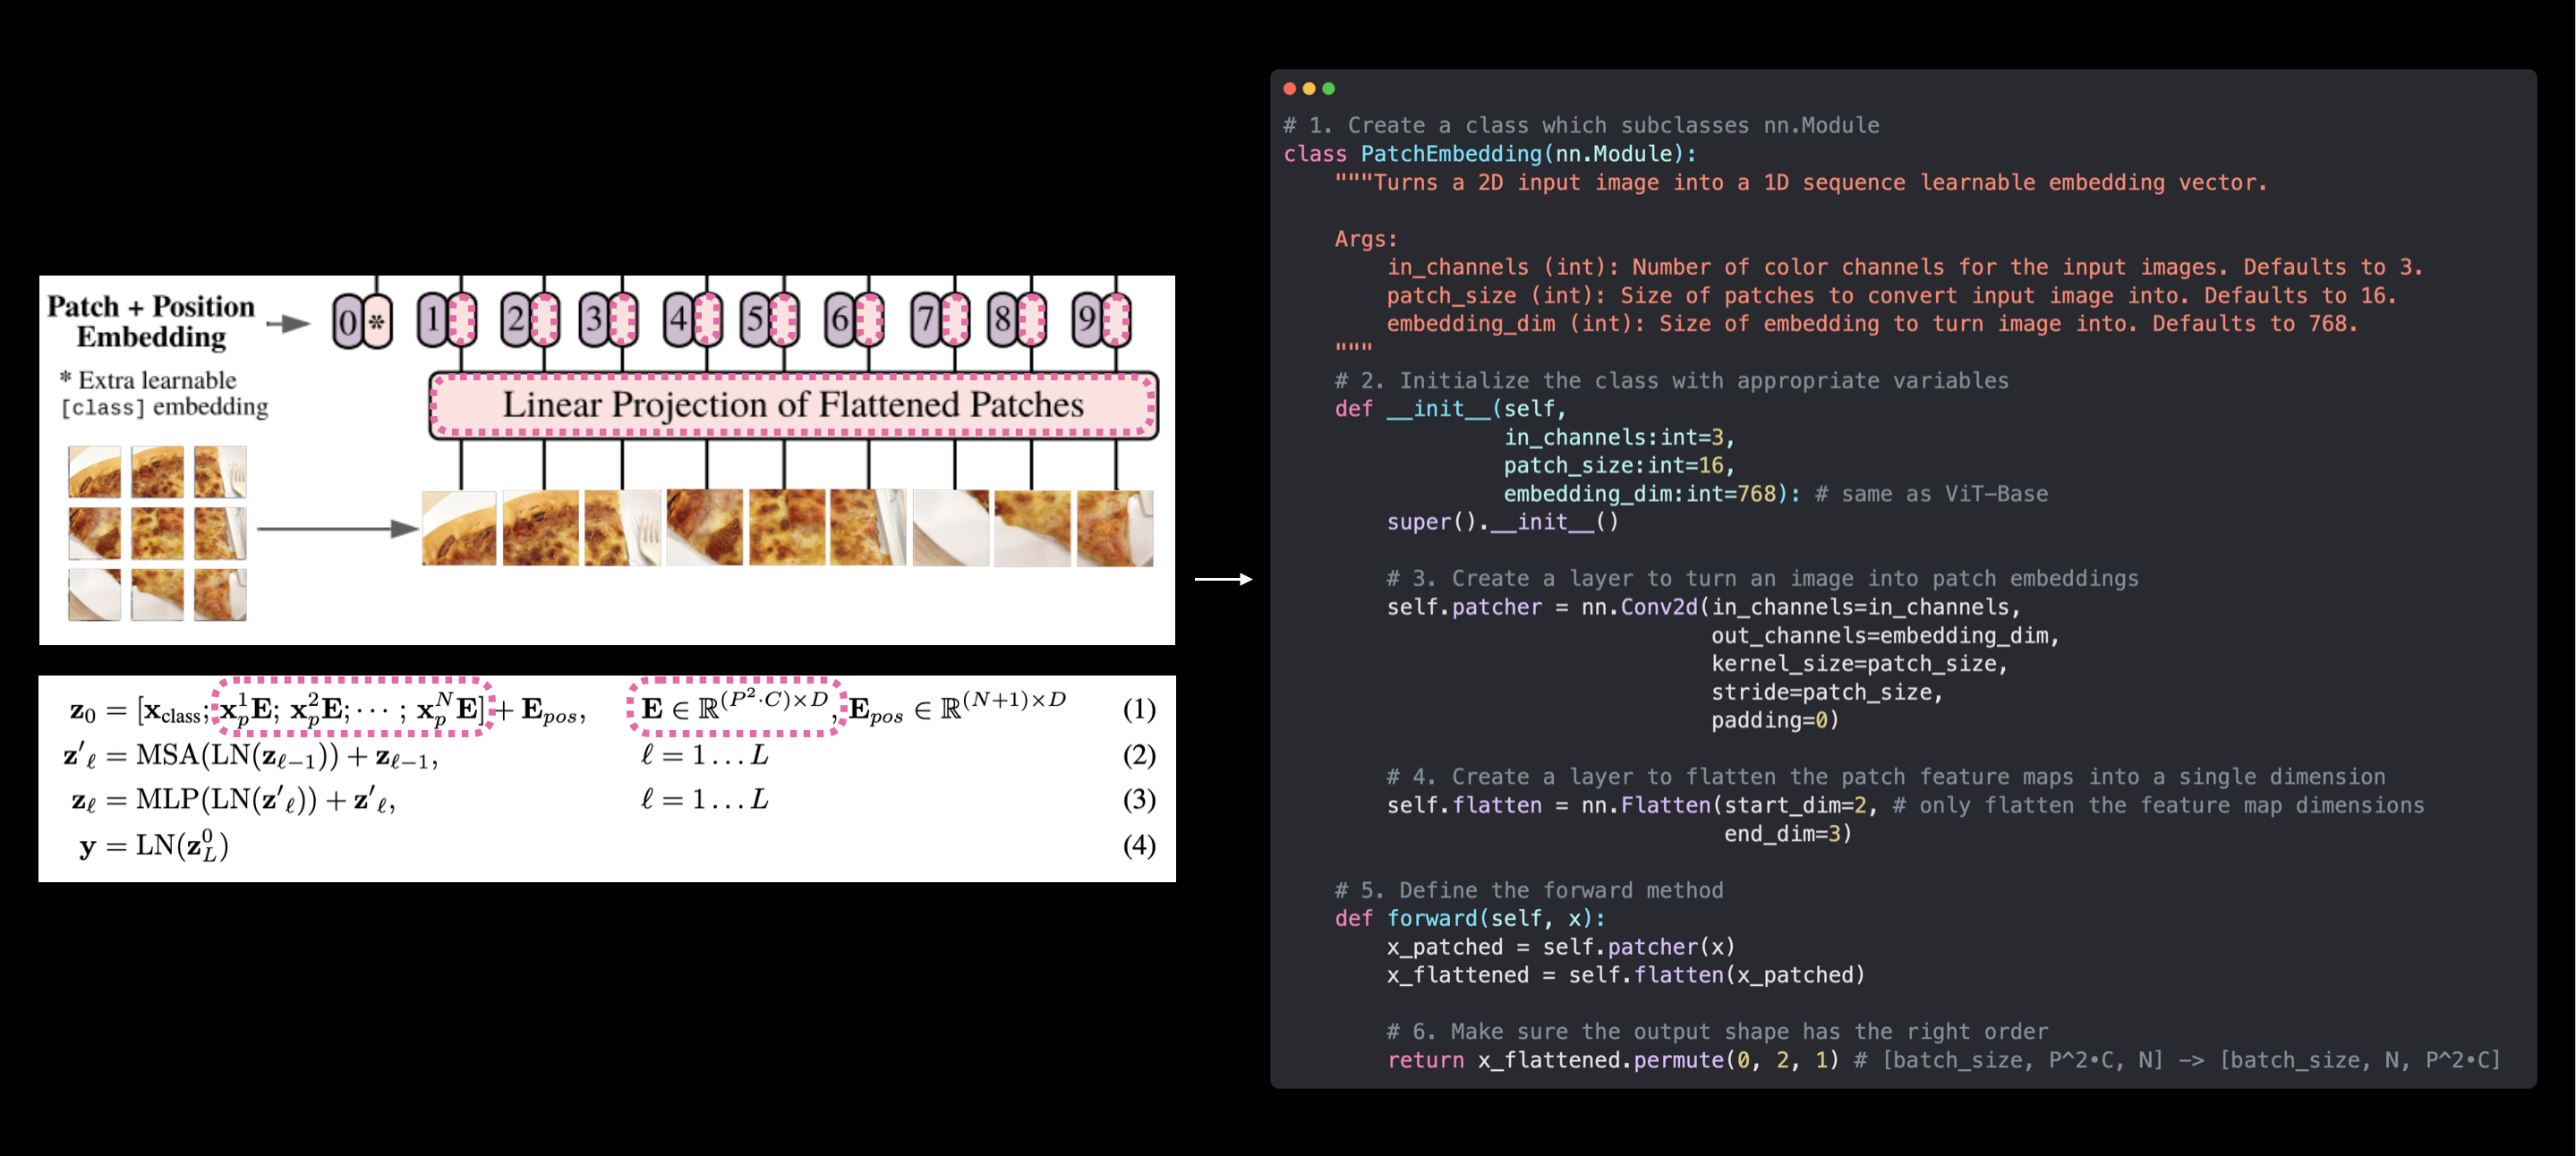
\includegraphics[width=1\linewidth]{figures/vit_patch_class_emb}
	\end{figure}

		
	\end{block}
\end{frame}
%==========================================================================================
\begin{frame}
	\frametitle{PyTorch - Paper Replicating}
	\begin{block}{Vamos replicar a equação 01 - Criando a incorporação do token de classe}
		Fizemos a incorporação do patch de imagem, hora de começar a trabalhar na classe de incorporação de token. \\
		Ou $\mathbf{x}_\text {class }$ da equação 1.
	\begin{figure}
		\centering
		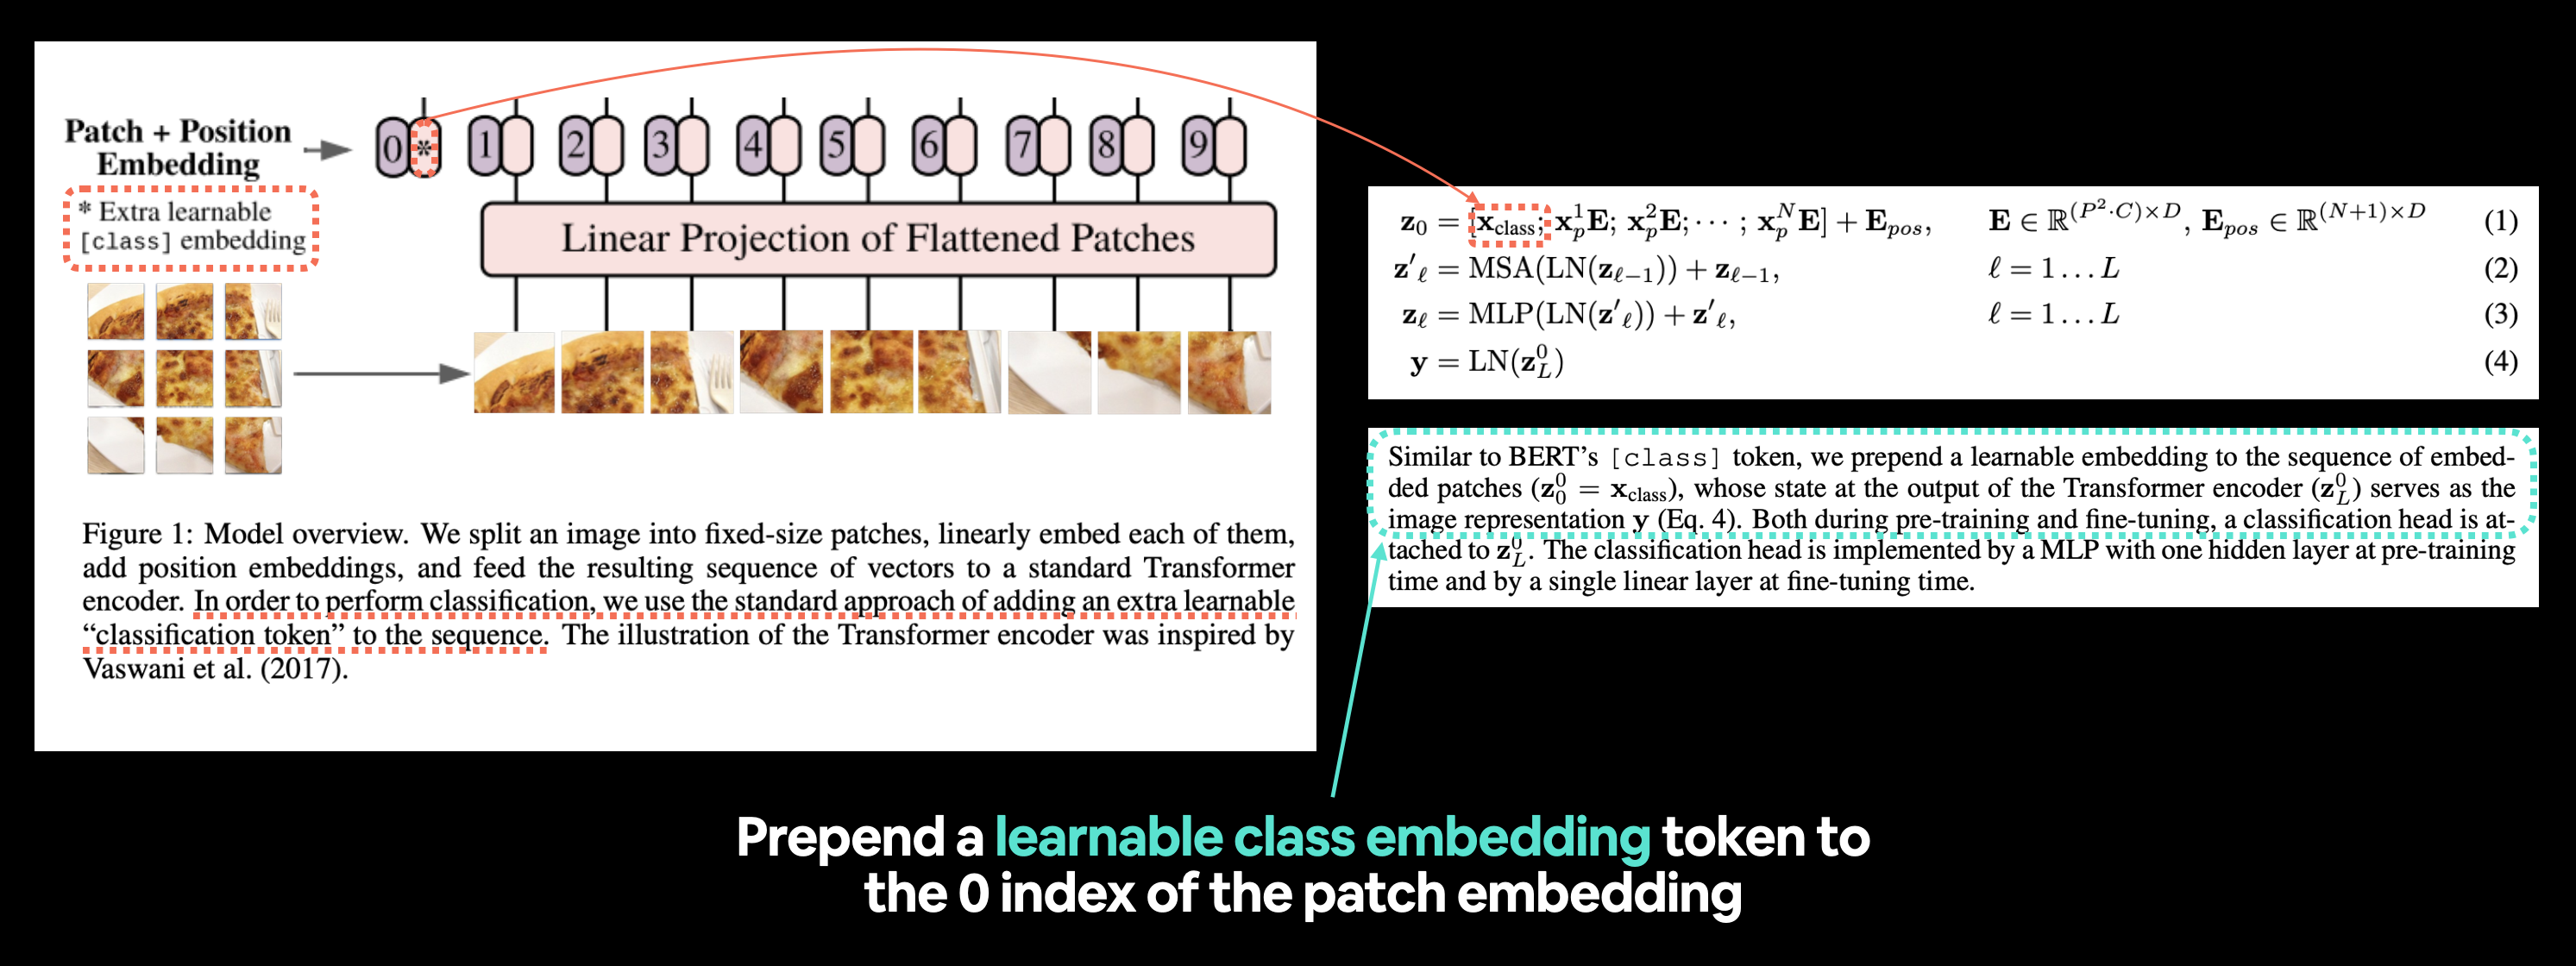
\includegraphics[width=1\linewidth]{figures/class_token}
	\end{figure}
			
		
	\end{block}
\end{frame}
%==========================================================================================

\begin{frame}
	\frametitle{PyTorch - Paper Replicating}
	\begin{block}{Vamos replicar a equação 01 - Criando a incorporação do token de classe}
		Esquerda: Figura 1 do documento ViT com o "token de classificação" ou token de incorporação [class] que vamos recriar em destaque.
		
		Direita: Equação 1 e seção 3.1 do documento ViT que se relacionam ao token de incorporação de classe que pode ser aprendido.
		\begin{figure}
			\centering
			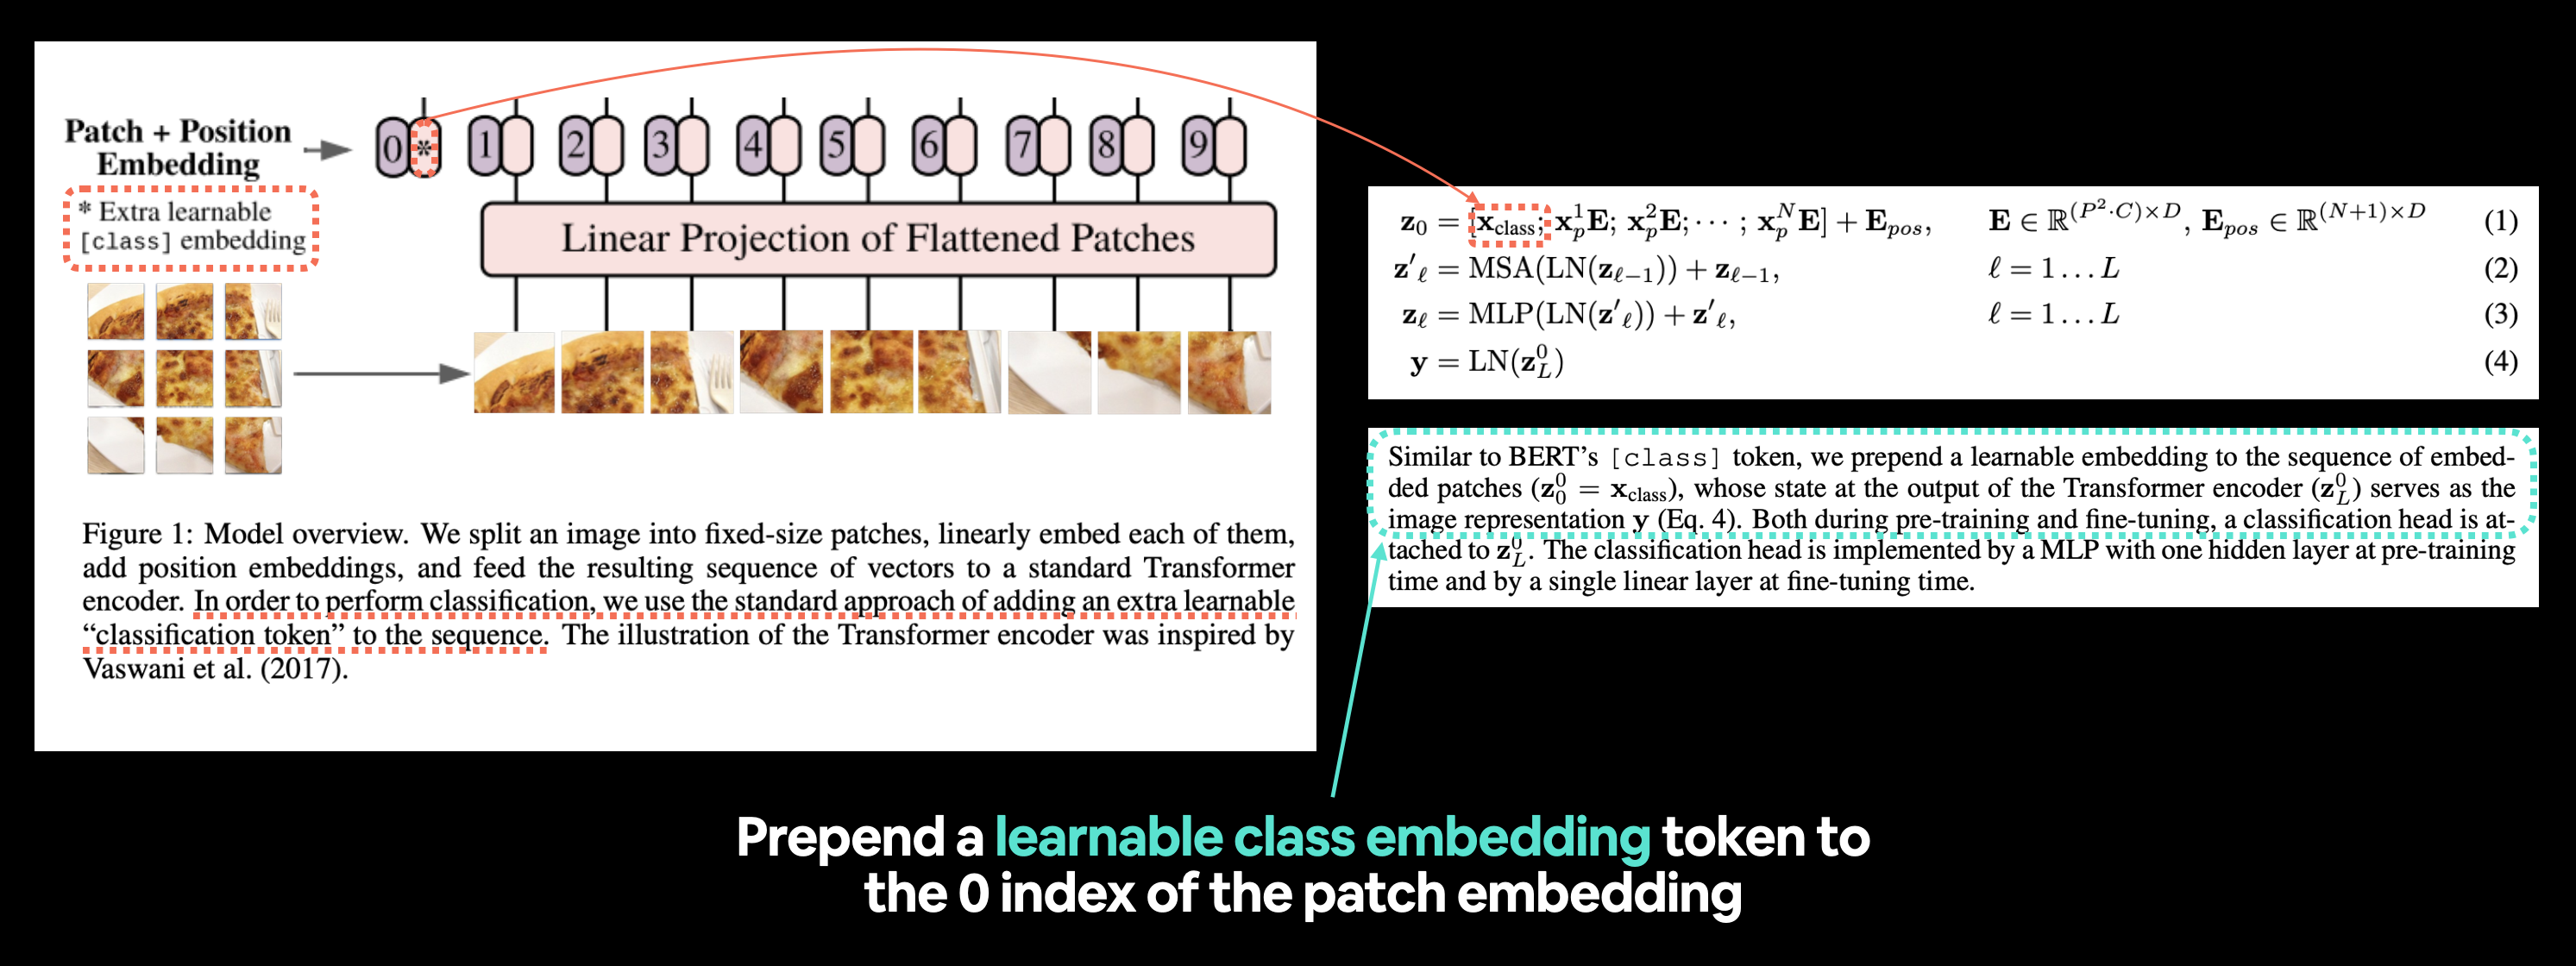
\includegraphics[width=1\linewidth]{figures/class_token}
		\end{figure}
		
		
	\end{block}
\end{frame}
%==========================================================================================

\begin{frame}
	\frametitle{PyTorch - Paper Replicating}
	\begin{block}{Equação 01 - Criando a incorporação do token de classe}
		Lendo o segundo parágrafo da seção 3.1 do artigo do ViT, vemos a seguinte descrição:
		
		Semelhante ao token `[ class ]` do BERT, acrescentamos uma incorporação que pode ser aprendida à sequência de patches incorporados $\left(\mathbf{z}_{0}^{0}=\mathbf{x}_{\text { classe }}\right)$, cujo estado na saída do codificador Transformer $\left(\mathbf{z}_{L}^{0}\right)$ serve como representação da imagem $\mathbf{y}$ (Eq. 4).
		
		\textbf{Observação:} [BERT](https://arxiv.org/abs/1810.04805) (Representações de Codificador Bidirecional de Transformers) é um dos trabalhos originais de pesquisa de aprendizado de máquina para usar a arquitetura Transformer para obter resultados excelentes em ambientes naturais tarefas de processamento de linguagem (NLP) e é onde se originou a ideia de ter um token [ class ] no início de uma sequência, class sendo uma descrição para a classe de "classificação" à qual a sequência pertencia.
		
		Portanto, precisamos "pré-preparar uma incorporação apreensível para a sequência de patches incorporados".
		
	\end{block}
\end{frame}

%==========================================================================================

\begin{frame}
	\frametitle{PyTorch - Paper Replicating}
	\begin{block}{Vamos replicar a equação 01 - Criando a incorporação do token de classe}
		
		Agora ja adicionamos a classe de token, mudando o shape de 196 para 197
		\begin{figure}
			\centering
			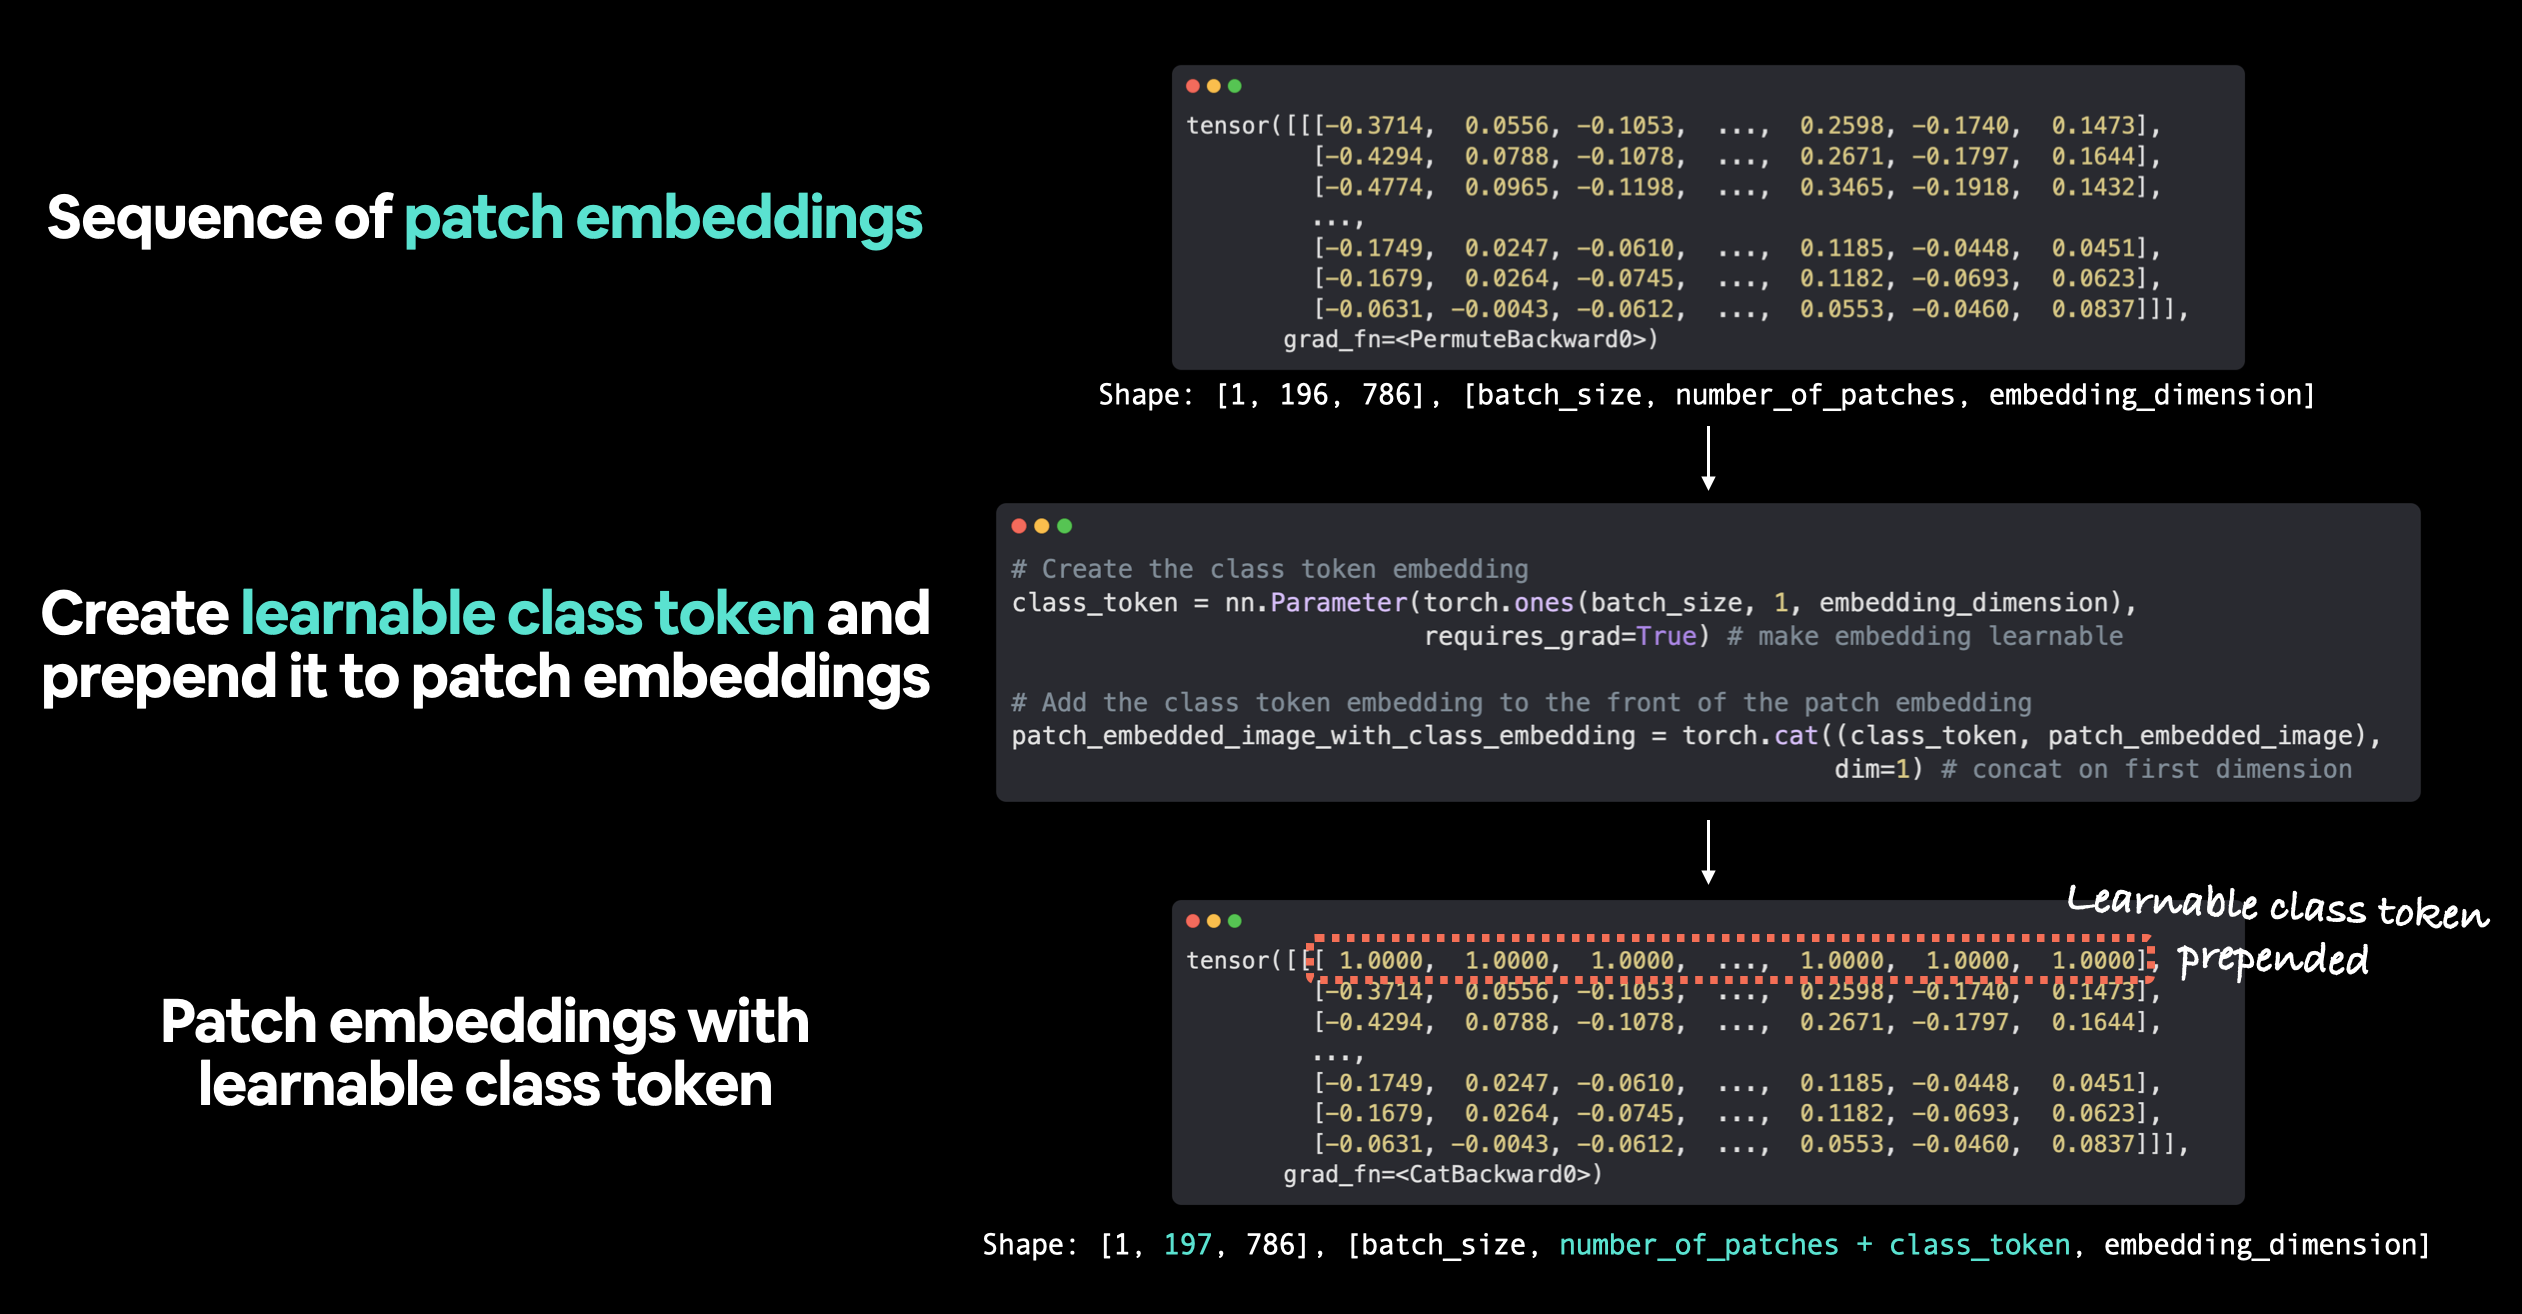
\includegraphics[width=0.8\linewidth]{figures/patch_embedding}
		\end{figure}
		
		
	\end{block}
\end{frame}

%==========================================================================================
\begin{frame}
	\frametitle{PyTorch - Paper Replicating}
	\begin{block}{Vamos replicar a equação 01 - Criando a position embedding}
		Bem, temos a incorporação de token de classe e a incorporação de patch, agora como podemos criar a incorporação de posição?
		
		Ou $\mathbf{E}_{\text {pos }}$ da equação 1 onde $E$ significa "embedding".
	\begin{figure}
		\centering
		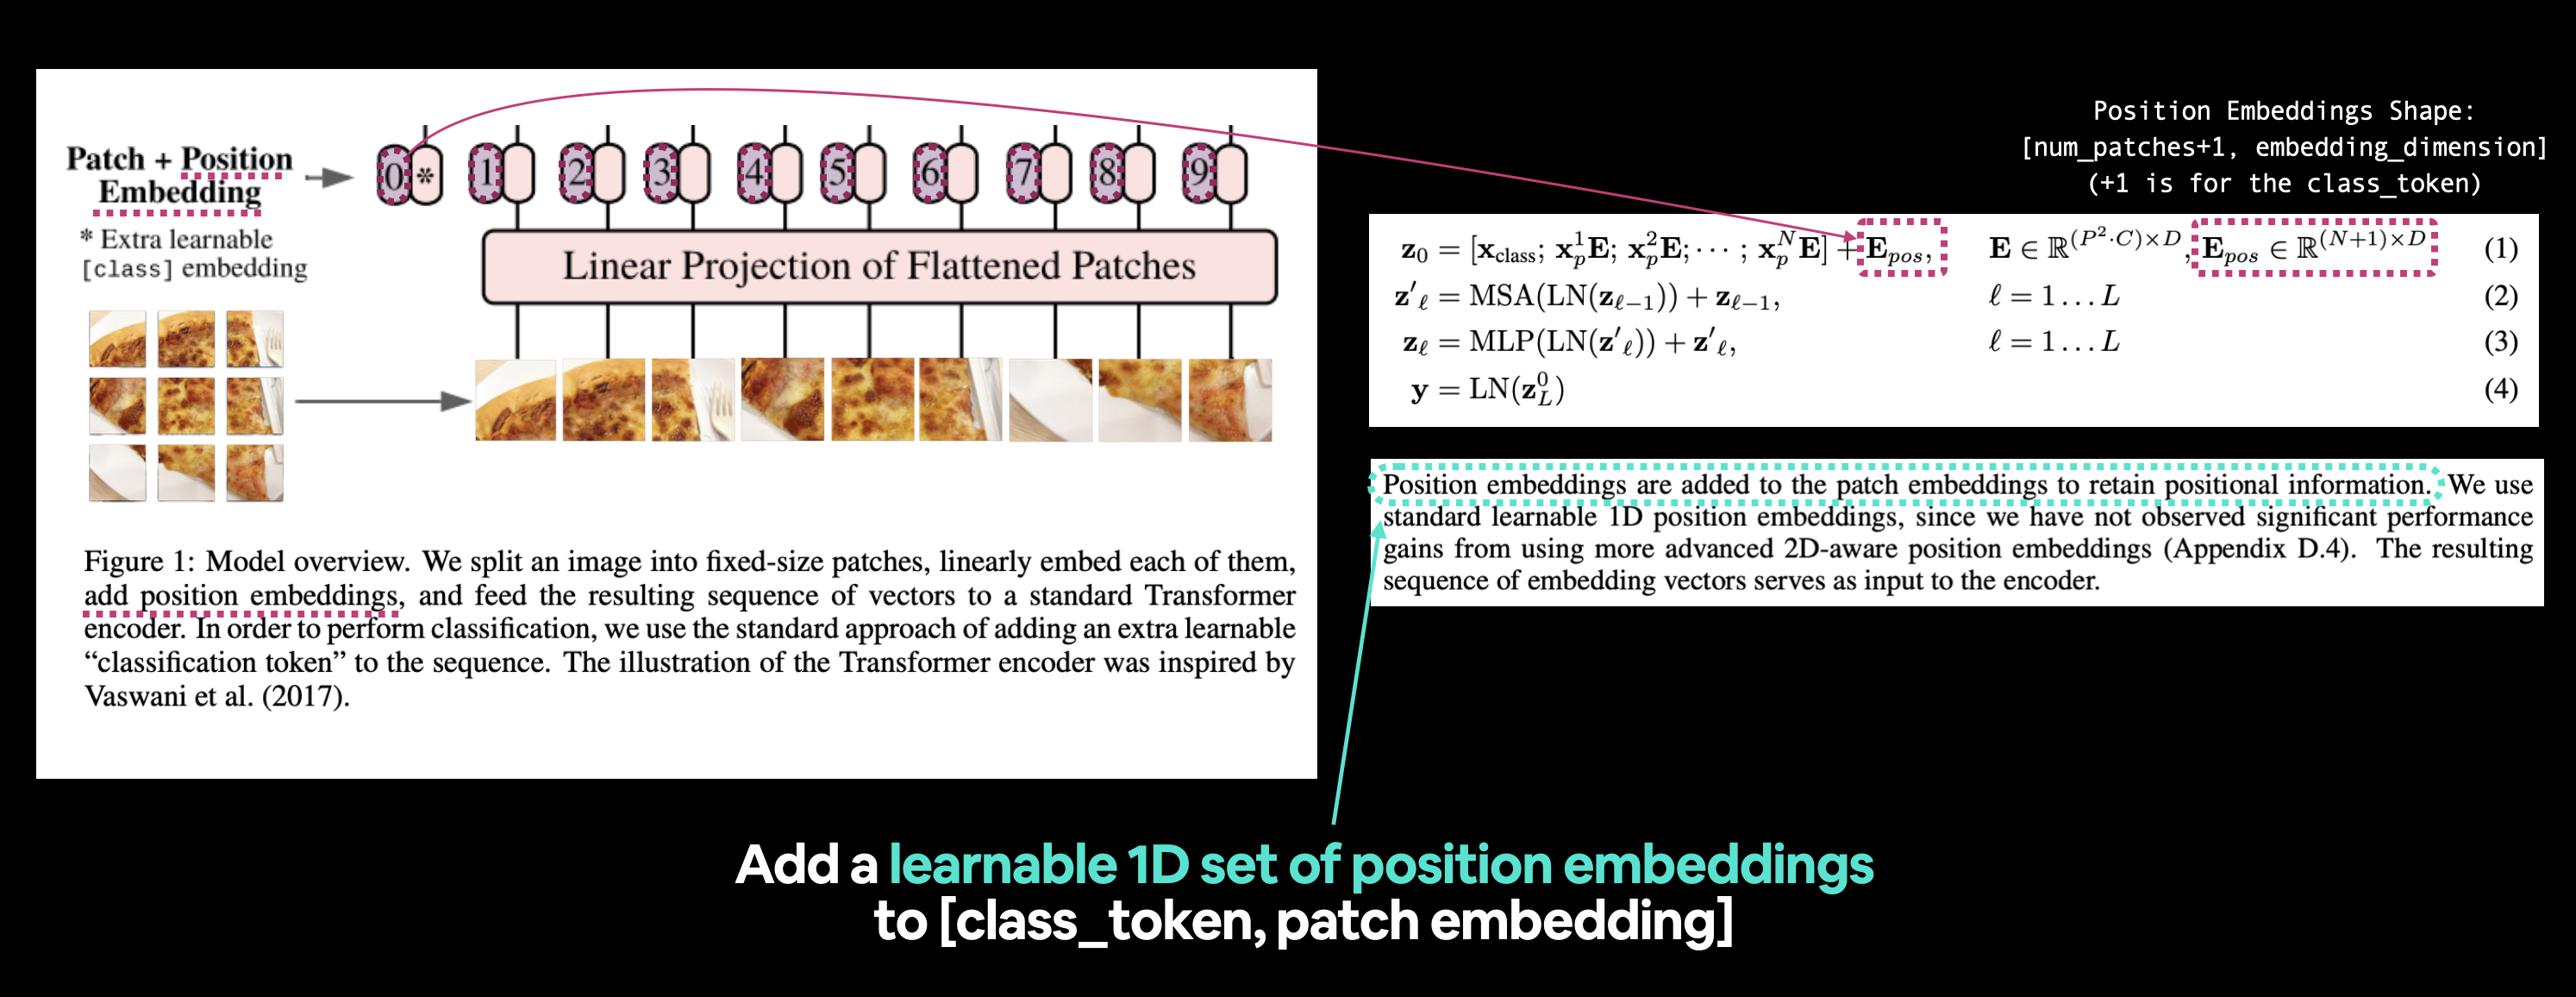
\includegraphics[width=1\linewidth]{figures/position_embedding}
	\end{figure}
	\end{block}
\end{frame}
%==========================================================================================
%==========================================================================================
\begin{frame}
	\frametitle{PyTorch - Paper Replicating}
	\begin{block}{Vamos replicar a equação 01 - Criando a position embedding}
		\begin{figure}
			\centering
			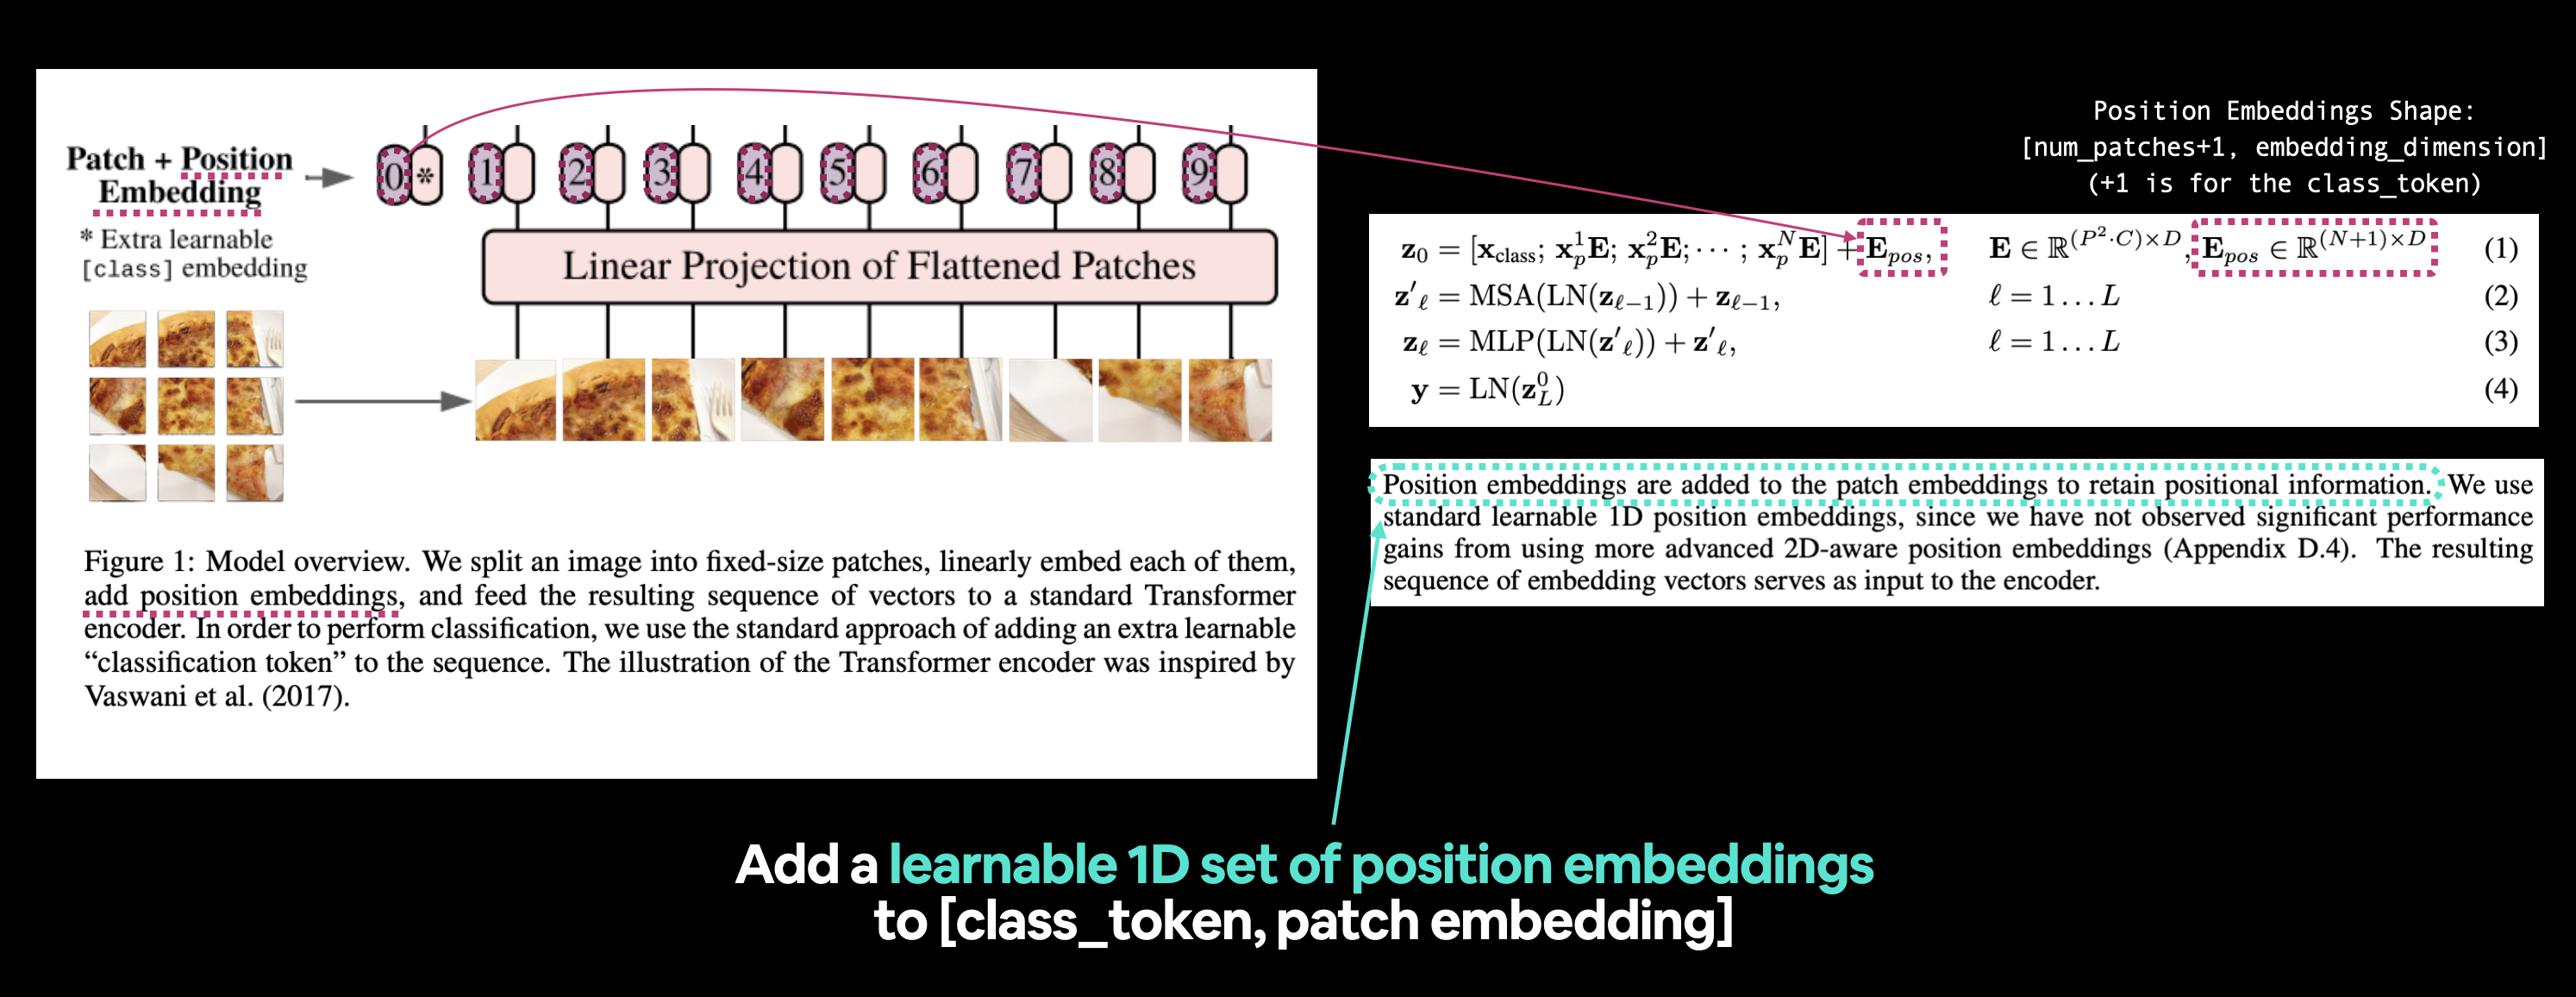
\includegraphics[width=1\linewidth]{figures/position_embedding}
		\end{figure}
		
		Esquerda: Figura 1 do documento ViT com a incorporação de posição que vamos recriar destacada. \\ Direita: Equação 1 e seção 3.1 do documento ViT que se relacionam com a incorporação de posição.
	\end{block}
\end{frame}
%==========================================================================================
\begin{frame}
	\frametitle{PyTorch - Paper Replicating}
	\begin{block}{Vamos replicar a equação 01 - Criando a position embedding}
	Vamos descobrir mais lendo a seção 3.1 do artigo do ViT (em negrito): \\
	As incorporações de posição são adicionadas às incorporações de patch para reter as informações posicionais. Usamos\textbf{ embeddings de posição 1D apreensíveis padrão}, já que não observamos ganhos significativos de desempenho com o uso de incorporações de posição 2D mais avançadas (Apêndice D.4). A sequência resultante de vetores de incorporação serve como entrada para o codificador.
	
	Por "reter informações posicionais", os autores querem que a arquitetura saiba em que "ordem" os patches vêm. Assim, o patch dois vem depois do patch um e o patch três vem depois do patch dois e assim por diante.
	
	Esta informação posicional pode ser importante ao considerar o que está em uma imagem (sem informação posicional, uma sequência achatada pode ser vista como sem ordem e, portanto, nenhum patch se relaciona com qualquer outro patch).
	
	Vamos visualizar nossas incorporações atuais.
	\end{block}
\end{frame}

%==========================================================================================
\begin{frame}
	\frametitle{PyTorch - Paper Replicating}
	\begin{block}{Vamos replicar a equação 01 - Criando a position embedding}
		\begin{figure}
			\centering
			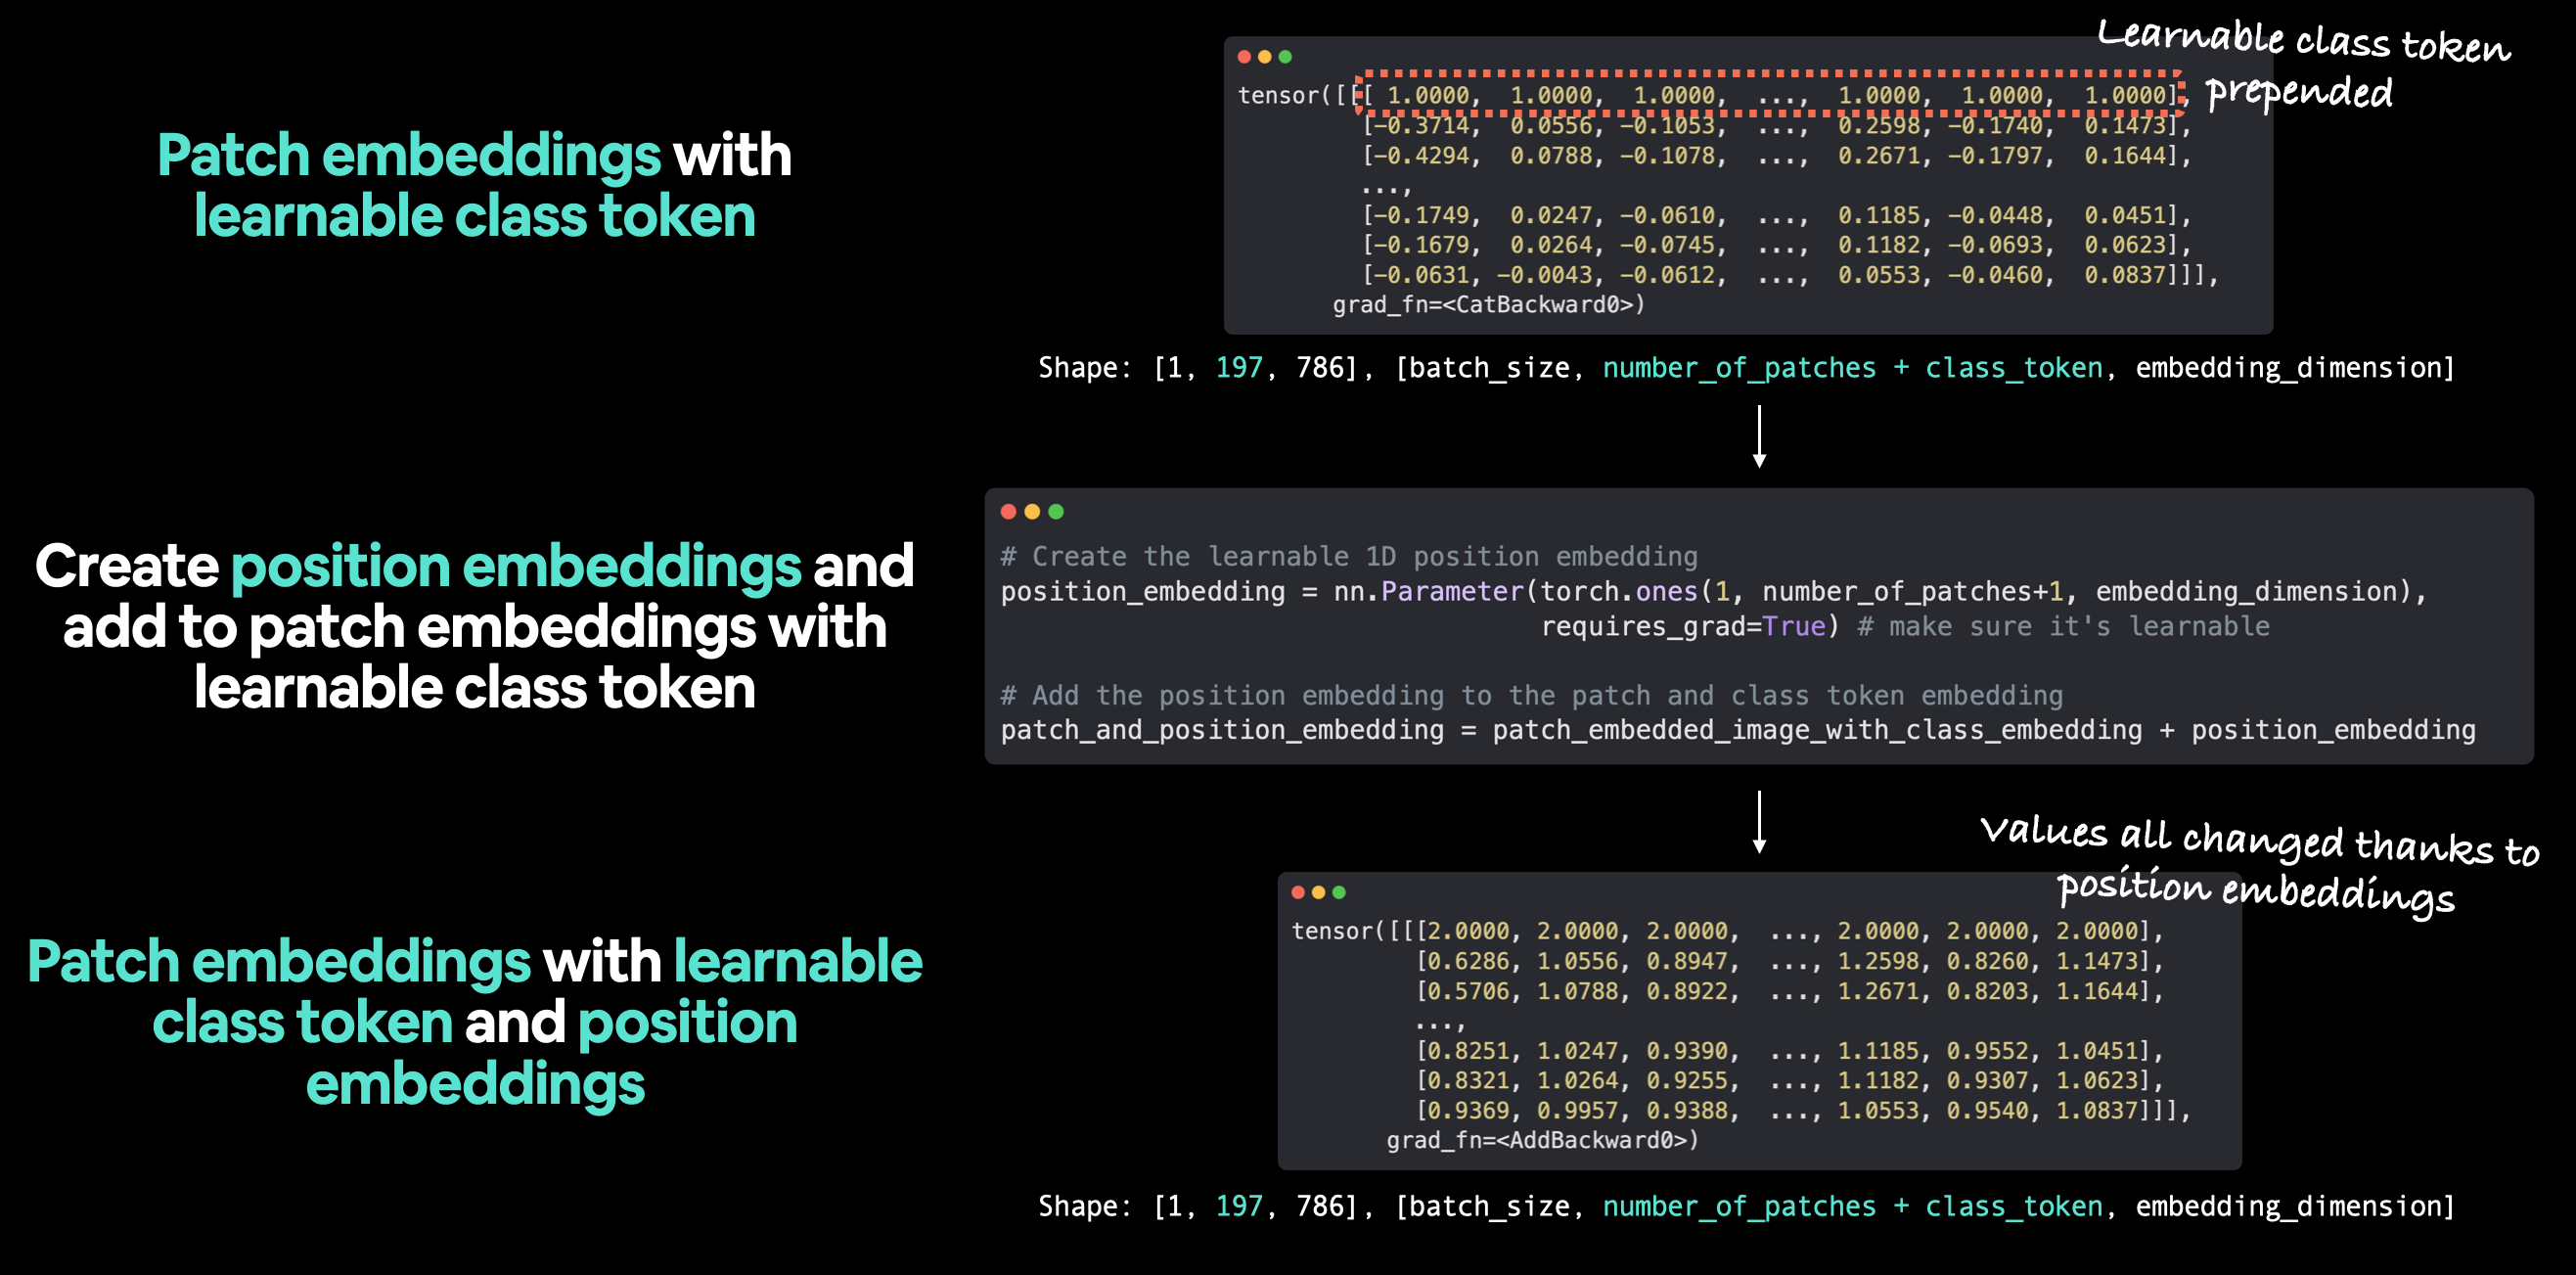
\includegraphics[width=1\linewidth]{figures/position_embedding_post}
		\end{figure}
		
	\end{block}
\end{frame}
%==========================================================================================
\begin{frame}
	\frametitle{PyTorch - Paper Replicating}
	\begin{block}{Vamos replicar a equação 01 - Juntando tudo: da imagem à embedding}
		\begin{itemize}
			\item Definir o tamanho do patch (usaremos '16', pois é amplamente utilizado em todo o artigo e para ViT-Base).
			\item Obtendo uma única imagem, imprimindo sua forma e armazenando sua altura e largura.
			\item Adicionar uma dimensão de lote à imagem única para que seja compatível com nossa camada PatchEmbedding.
			\item Criando uma camada PatchEmbedding (aquela que fizemos na seção 4.5) com um patch\_size=16 e embedding\_dim=768 (da Tabela 1 para ViT-Base).
		\end{itemize}
		
	\end{block}
\end{frame}
%==========================================================================================
\begin{frame}
	\frametitle{PyTorch - Paper Replicating}
	\begin{block}{Vamos replicar a equação 01 - Juntando tudo: da imagem à embedding}
		\begin{itemize}
			\item Passar a imagem única através da camada PatchEmbedding em 4 para criar uma sequência de embeddings de patch.
			\item Criar uma incorporação de token de classe como na seção 4.6.
			\item Preceder o emebdding do token de classe aos embeddings de patch criados na etapa 5.
			\item Criando uma incorporação de posição como na seção 4.7.
			\item Adicionando a incorporação de posição ao token de classe e incorporações de patch criadas na etapa 7.
		\end{itemize}
		
	\end{block}
\end{frame}
%==========================================================================================
\begin{frame}
	\frametitle{PyTorch - Paper Replicating}
	\begin{block}{Vamos replicar a equação 01 - Juntando tudo: da imagem à embedding}
		\begin{figure}
			\centering
			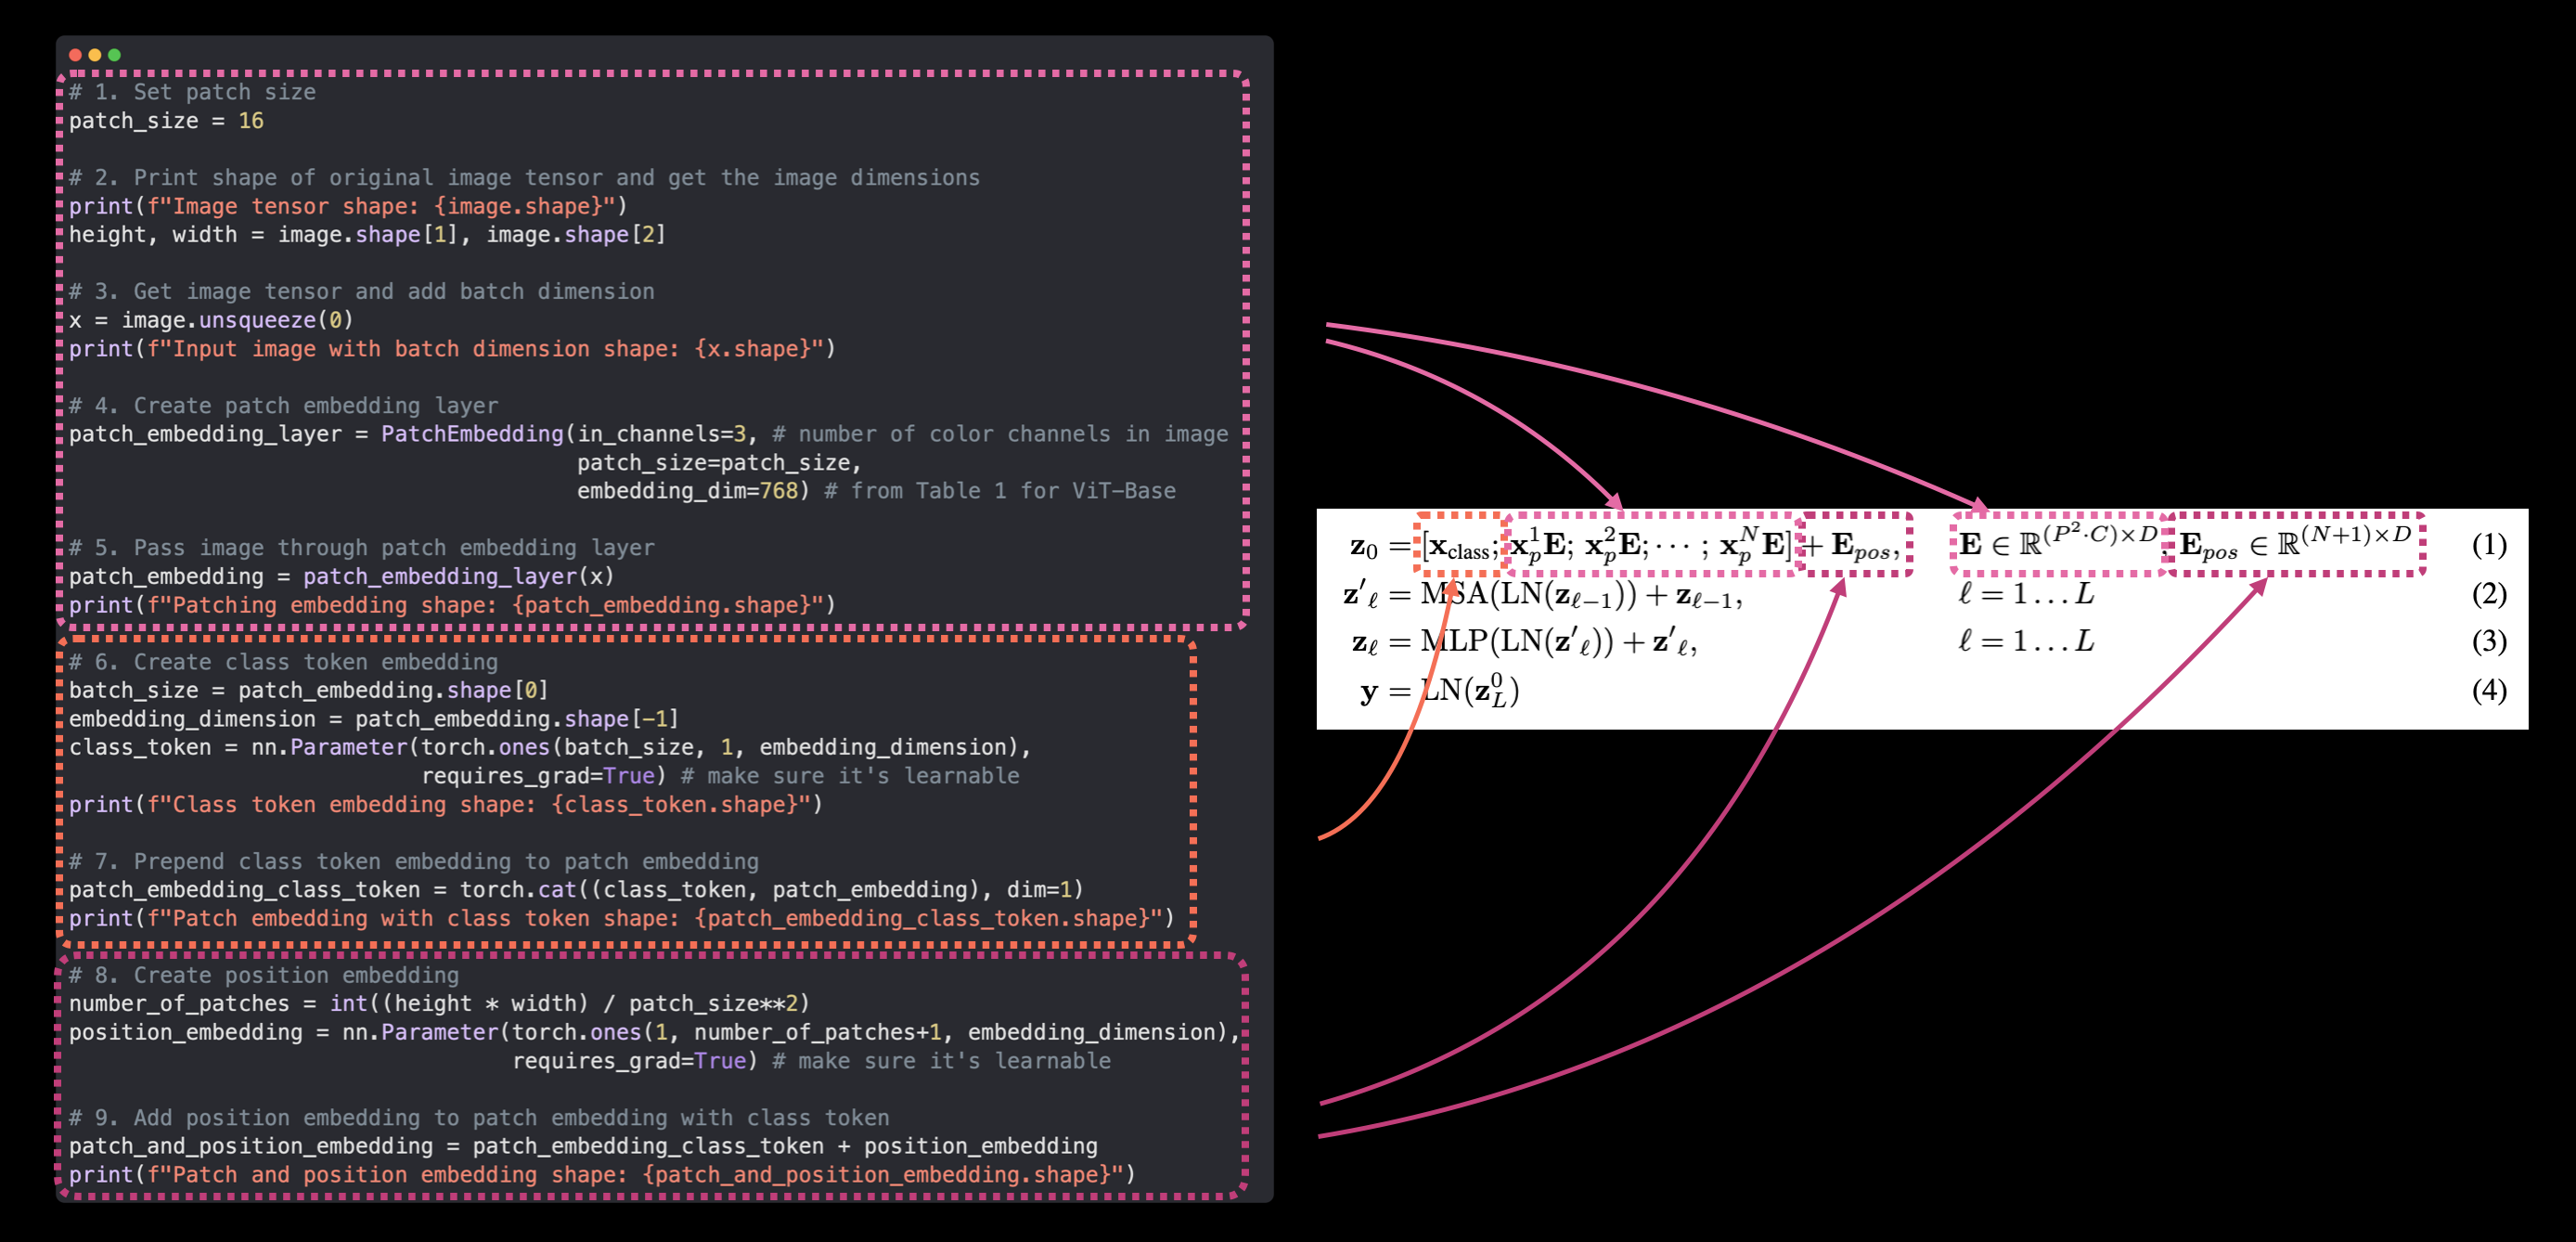
\includegraphics[width=1\linewidth]{figures/position_embedding_post1}
		\end{figure}
	\href{https://github.com/mafaldasalomao/pavic_treinamento_ml/raw/main/Machine_Learning/figures/08-vit-paper-architecture-animation-full-architecture.gif}{\beamergotobutton{Image}} 
	\end{block}
\end{frame}
%==========================================================================================
\begin{frame}
	\frametitle{PyTorch - Paper Replicating}
	\begin{block}{Equation 2: Multi-Head Attention (MSA)}
		
		\begin{figure}
			\centering
			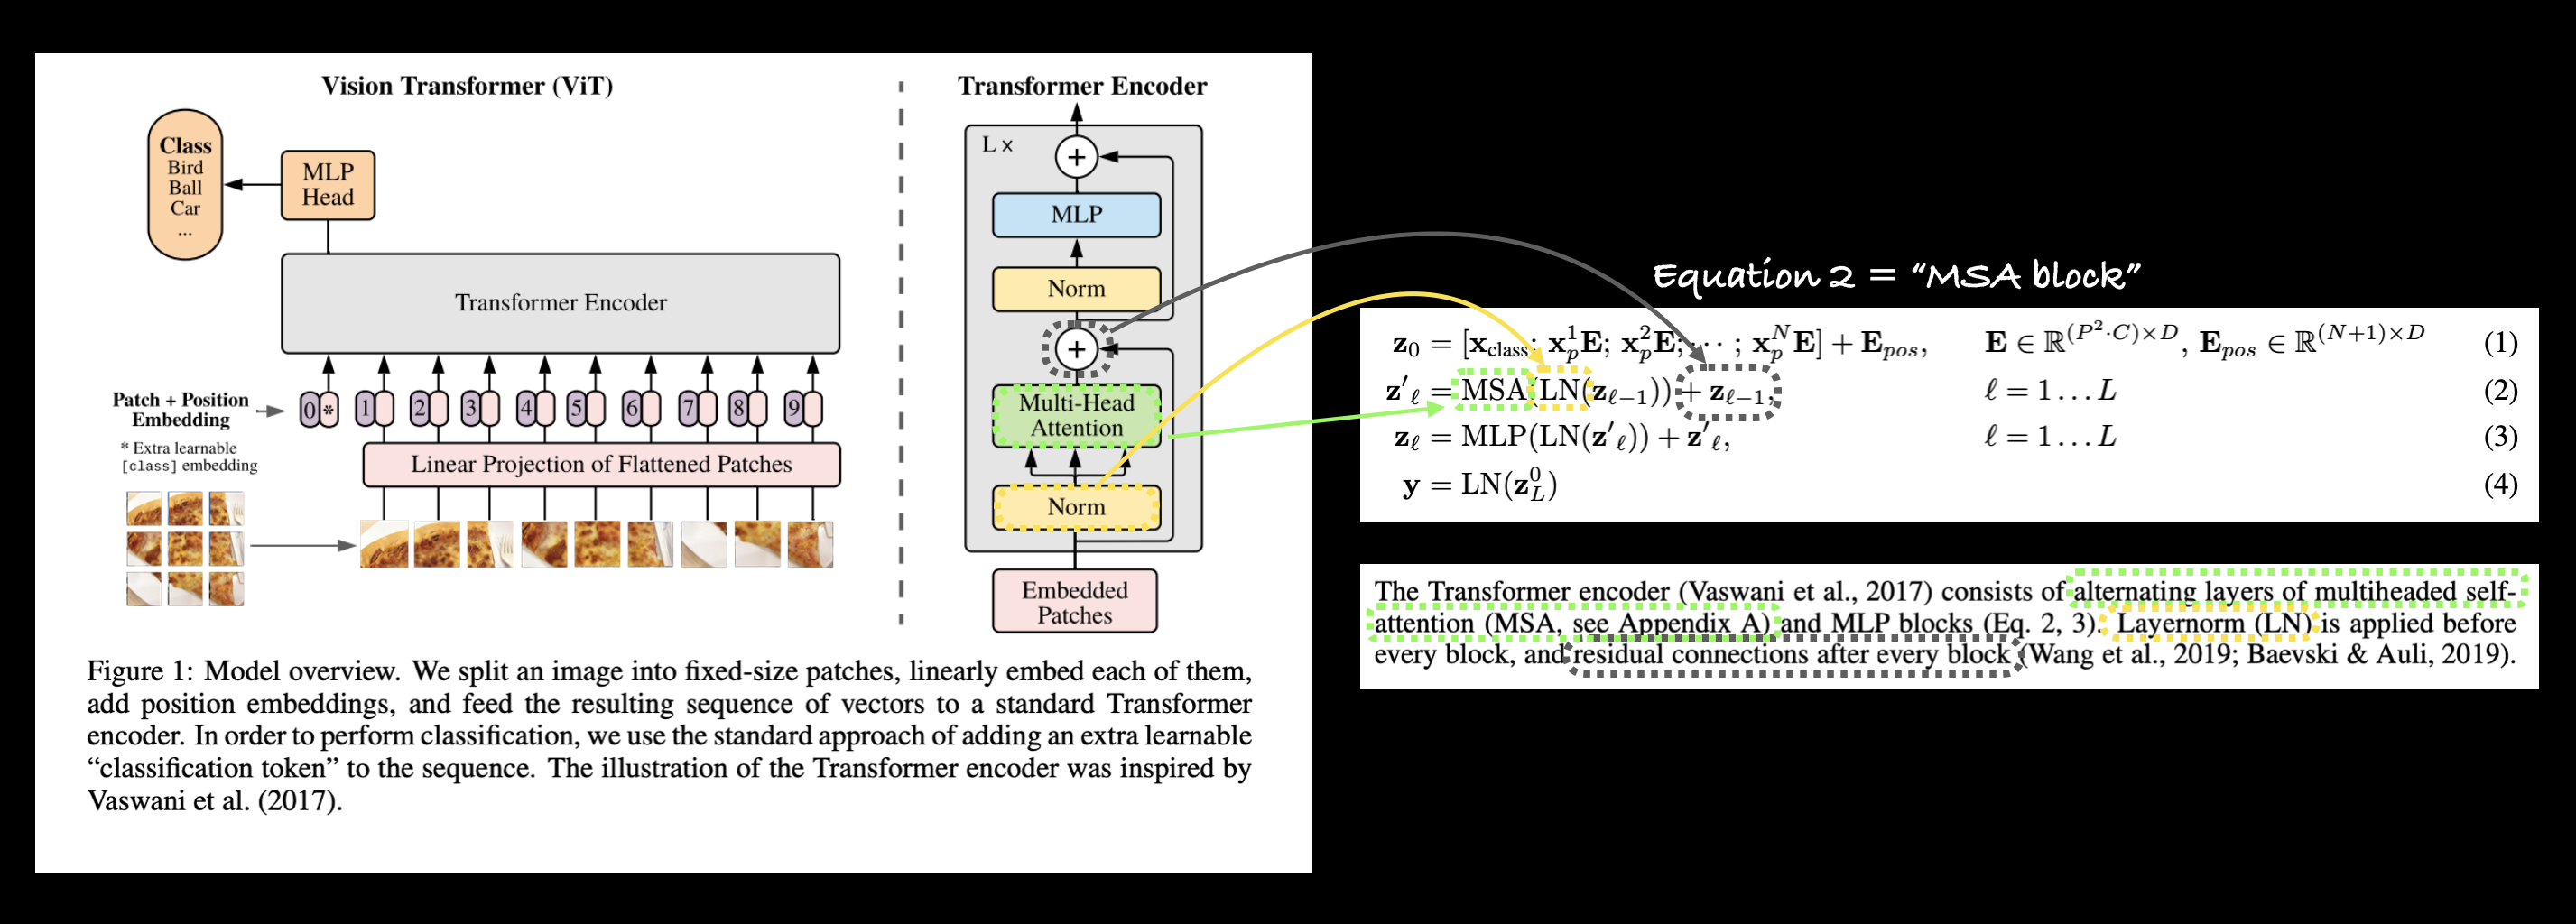
\includegraphics[width=0.7\linewidth]{figures/msa}
		\end{figure}
		
	\end{block}
\end{frame}
%==========================================================================================
\begin{frame}
	\frametitle{Métodos de Inicialização de Pesos}
	\begin{block}{Distribuição Uniforme Aleatória}
		\begin{itemize}
			\item $y \in [0, 1]$ 
			\item Inicializa todos o pesos com uma Distribuição Uniforme Aleatória 
			\item Quebra a simetria
		\end{itemize}
			$	y = np.random.rand(H, W)$
		\begin{figure}
			\centering
			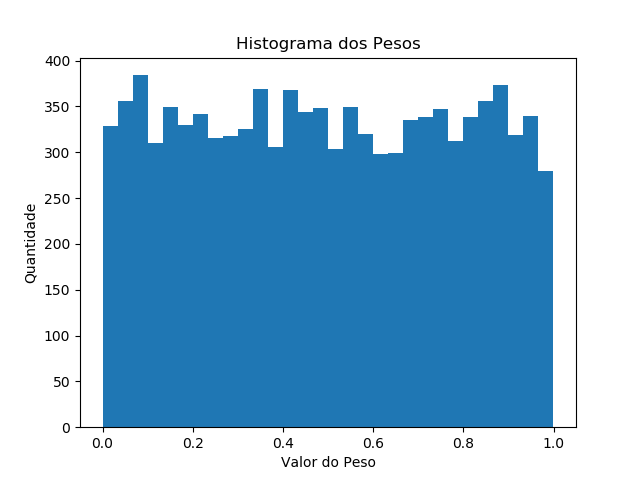
\includegraphics[width=0.5\linewidth]{figures/pesos_uniform.png}
		\end{figure}
	\end{block}
\end{frame}
%==========================================================================================

\begin{frame}
	\frametitle{Métodos de Inicialização de Pesos}
	\begin{block}{Distribuição Normal}
		\begin{itemize}
			\item $y \in [-\infty, +\infty]$ 
			\item Inicializa todos o pesos com uma Distribuição Normal informando média e desvio padrão 
			\item Ajuda a quebrar a simetria da rede
		\end{itemize}
		$	y = np.random.randn(H, W)$
		\begin{figure}
			\centering
			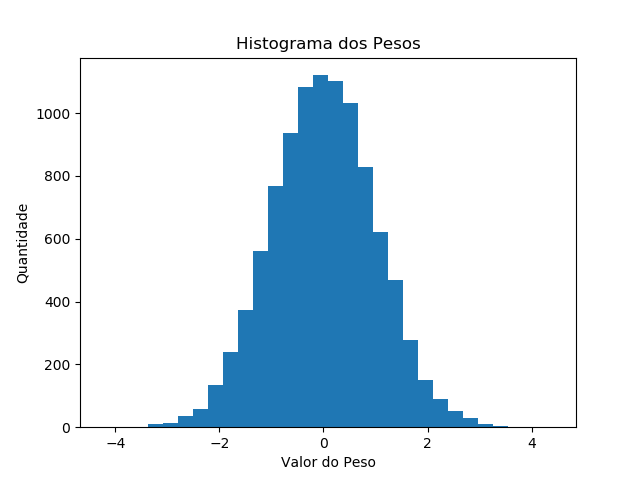
\includegraphics[width=0.5\linewidth]{figures/pesos_normal.png}
		\end{figure}
	\end{block}
\end{frame}
%==========================================================================================
\begin{frame}
	\frametitle{Métodos de Inicialização de Pesos}
	\begin{block}{Glorot Uniforme}
		\begin{columns}
			\begin{column}{0.6 \textwidth}
				\begin{itemize}
					\item $y \in [-\sigma, +\sigma]$
					\item Conhecida como \textbf{Xavier Uniforme}
					\item Leva em consideração o tamanho das camadas
					\item Ajuda a quebrar a simetria
				\end{itemize}
				$	y = 2 * \sigma * np.random.rand(H, W) - \sigma$ \\
				Sendo:
				$\sigma = \sqrt{\frac{6}{in + out}}$ \\
				$in$ é a quantidade de neurônio da camada anterior e $out$ a quantidade de neurônio da camada atual
			\end{column}
		\begin{column}{0.4 \textwidth}
			\begin{itemize}
				\item Torna a convergência mais rápida e eficiente
				\item Uma das melhores inicializações de peso
			\end{itemize}
			\begin{figure}
				\centering
				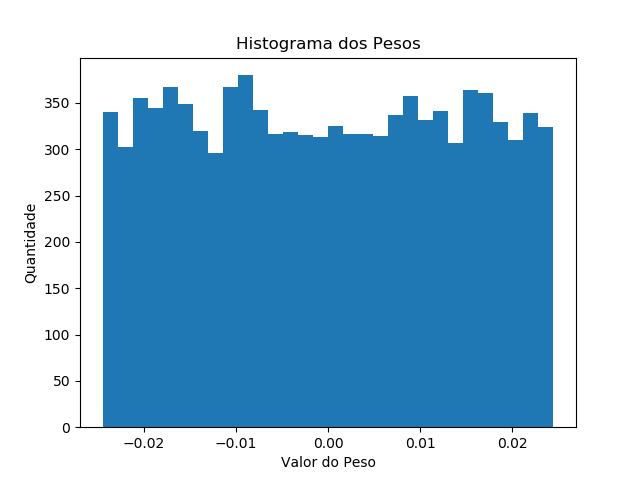
\includegraphics[width=1\linewidth]{figures/pesos_glorot_uniform.png}
			\end{figure}
		\end{column}
		\end{columns}
	\end{block}
\end{frame}
%==========================================================================================
\begin{frame}
	\frametitle{Métodos de Inicialização de Pesos}
	\begin{block}{Glorot Normal}
		\begin{columns}
			\begin{column}{0.6 \textwidth}
				\begin{itemize}
					\item $y \in [-\sigma, +\sigma]$
					\item Conhecida como \textbf{Xavier Normal}
					\item Leva em consideração o tamanho das camadas
					\item Ajuda a quebrar a simetria
				\end{itemize}
				$	y =  \sigma * np.random.randn(H, W) - \sigma$ \\
				Sendo:
				$\sigma = \sqrt{\frac{2}{in + out}}$ \\
				$in$ é a quantidade de neurônio da camada anterior e $out$ a quantidade de neurônio da camada atual
			\end{column}
			\begin{column}{0.4 \textwidth}
				\begin{itemize}
					\item Torna a convergência mais rápida e eficiente
					\item Uma das melhores inicializações de peso
				\end{itemize}
				\begin{figure}
					\centering
					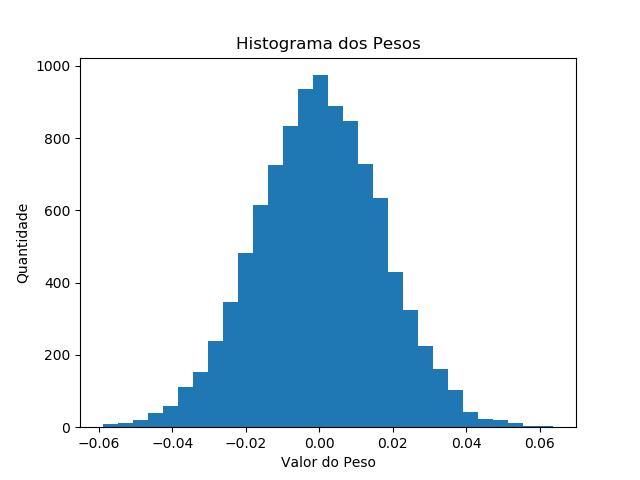
\includegraphics[width=1\linewidth]{figures/pesos_glorot_normal.png}
				\end{figure}
			\end{column}
		\end{columns}
	\end{block}
\end{frame}
%==========================================================================================
\begin{frame}
	\frametitle{Métodos de Inicialização de Pesos}
	\begin{block}{Qual método de inicialização utilizar?}
	\begin{figure}
		\centering
		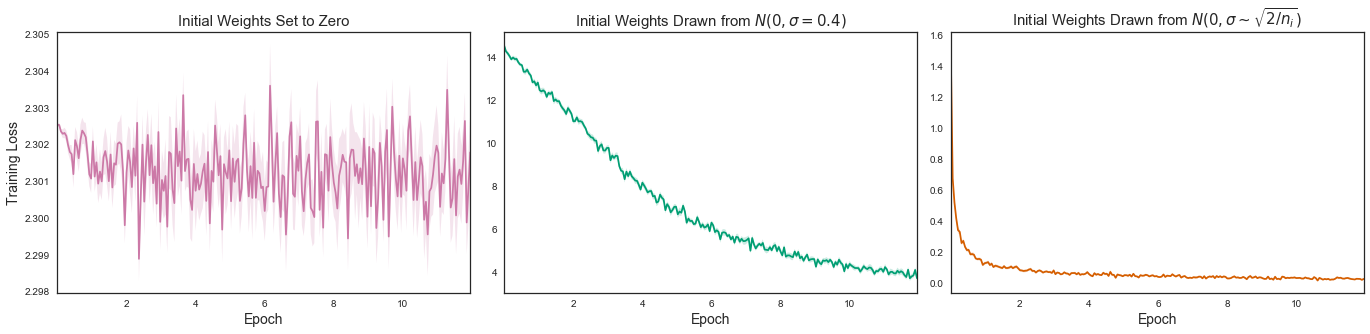
\includegraphics[width=1\linewidth]{figures/weights_init}
	\end{figure}
	Vamos ver isso na prática utilizando o notebook das Redes Neurais! \\
	Vamos refazer nossos experimentos e analisar os resultados
	\end{block}
\end{frame}
%==========================================================================================
\begin{frame}
	\frametitle{Métodos de Inicialização de Pesos}
	\begin{block}{Qual método de inicialização utilizar?}
		\begin{figure}
			\centering
			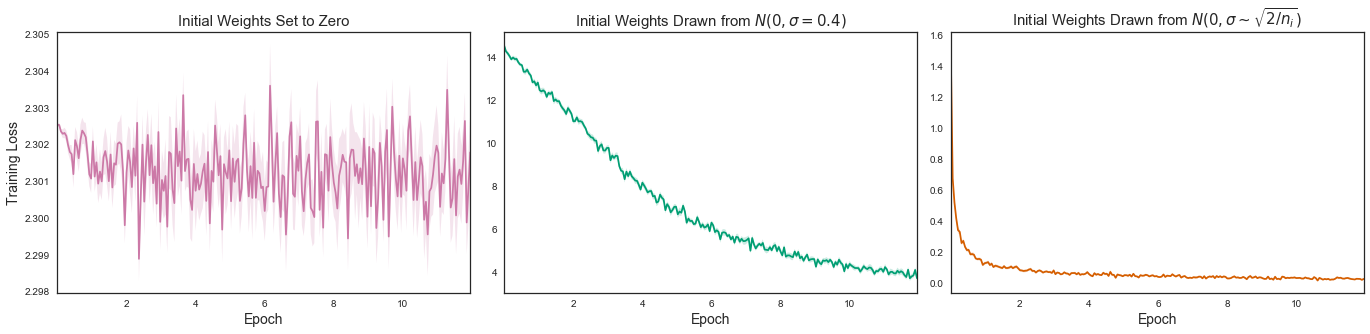
\includegraphics[width=1\linewidth]{figures/weights_init}
		\end{figure}
	\end{block}
\end{frame}
%==========================================================================================
\begin{frame}
	\frametitle{Técnicas de Regularização}
	\begin{block}{Dropout}
		\begin{itemize}
			\item Zerar aleatoriamente a ativação de alguns neurônios por camada utilizando uma probabilidade $p$
			\item Se $p=0.5$ é a probabilidade de zerar 50\% dos neurônios
			\item Cuidado para não tornar a rede ineficiente
			\item A cada iteração diferentes neurônios serão desabilitados, dando a ideia do treinamento de varias sub-redes
			\item os neurônios subsequentes não recebem dados de todos neurônios anteriores.
			\item Uma das melhores técnicas de regularização
			\item Só aplicado no banco de treinamento
			\item Só usado quando ocorre overfitting
		\end{itemize}
	\end{block}
\end{frame}
%==========================================================================================
\begin{frame}
	\frametitle{Técnicas de Regularização}
	\begin{block}{Dropout}
		\begin{figure}
			\centering
			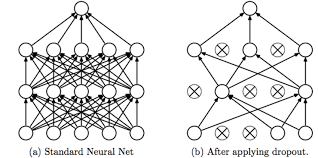
\includegraphics[width=1\linewidth]{figures/dropout}
		\end{figure}
	\end{block}
\end{frame}
%==========================================================================================
\begin{frame}
	\frametitle{Técnicas de Regularização}
	\begin{block}{Regularização L1}
		\begin{itemize}
			\item Criar uma rede menor capaz de resolver o problema
			\item Solução esparsas, atualizando alguns pesos e bias para zeros
			\item Semelhante ao Dropout
			\item Ela deixa apenas os atributos mais relevantes para a rede
			\item A rede é obrigada a aprender com pesos pequenos! E ter o mesmo resultado
			\item A dificuldade é estimar o $\lambda$
			\item Só usado quando ocorre overfitting
		\end{itemize}
	$$J = L(y, w, b) + \frac{\lambda}{m} \sum ||w||$$
	$L(y, w, b)$ é nossa Cost Function \\
	Na L1 é adicionado o termo $ \frac{\lambda}{m} \sum ||w||$  somar o valor absoluto dos pesos e multiplicar por um fator de regularização $\lambda$ e dividir pela Qtd. de amostras. Adicionado isso á nossa MSE, MAE,...
	\end{block}
\end{frame}
%==========================================================================================
\begin{frame}
	\frametitle{Técnicas de Regularização}
	\begin{block}{Regularização L1}
		A derivada da regularização... \\
		Vamos tomar como exemplo a MSE
		$$J = \frac{1}{2} \sum (y - \hat{y})^2 + \frac{\lambda}{m} \sum |w|$$
		A derivada da MSE é:
		$\frac{\partial J1}{\partial w} = -(y - \hat{y})x$ \\
		A derivada do termo pode ser dado por:
		$$\frac{\partial J2}{\partial w} =  \left\{\begin{matrix}
			+1, w > 0
			\\ 
			-1, w < 0
		\end{matrix}\right.$$
	Vamos aplicar isso na formula de atualização dos pesos:
	$w = w - \eta \frac{\partial J}{\partial w}$ Valor inicial - LR * derivada dos pesos 
	\end{block}
\end{frame}
%==========================================================================================

\begin{frame}
	\frametitle{Técnicas de Regularização}
	\begin{block}{Regularização L1}
		Vamos aplicar isso na formula de atualização dos pesos:
		$w = w - \eta \frac{\partial J}{\partial w}$ Valor inicial - LR * derivada dos pesos \\
		Agora... Já que a derivada da soma é a soma das derivadas \\
		$w = w - \eta [\frac{\partial J1}{\partial w} + \frac{\partial J2}{\partial w}]$ \\
		Agora vamos atualizar os pesos da seguinte forma:
		$$w =  \left\{\begin{matrix}
			w - \eta [-(y-\hat{y})x + \frac{\lambda}{m}], w > 0
			\\ 
			w - \eta [-(y-\hat{y})x - \frac{\lambda}{m}], w < 0
		\end{matrix}\right.$$
	\end{block}
\end{frame}
%==========================================================================================

\begin{frame}
	\frametitle{Técnicas de Regularização}
	\begin{block}{Regularização L2}
		\begin{itemize}
			\item Criar uma rede na qual nenhum atributo seja tão mais importante que os outros
			\item Diminui e espalha os valores dos pesos
			\item Mais utilizada que a L1
			\item Conhecida como Weight decay
			\item A dificuldade é estimar o $\lambda$
			\item Só usado quando ocorre overfitting
		\end{itemize}
		$$J = L(y, w, b) + \frac{\lambda}{2m} \sum w_i^2$$
	\end{block}
\end{frame}
%==========================================================================================
\begin{frame}
	\frametitle{Técnicas de Regularização}
	\begin{block}{Regularização L2}
		A derivada da regularização... \\
		Vamos tomar como exemplo a MSE
		$$J = \frac{1}{2} \sum (y - \hat{y})^2 + \frac{\lambda}{2m} \sum w_i^2$$
		A derivada da MSE é:
		$\frac{\partial J1}{\partial w} = -(y - \hat{y})x$ \\
		A derivada do termo pode ser dado por:
		$$\frac{\partial J2}{\partial w} =  \frac{\lambda w}{m}$$
		Vamos aplicar isso na formula de atualização dos pesos:
		$w = w - \eta \frac{\partial J}{\partial w}$ Valor inicial - LR * derivada dos pesos 
	\end{block}
\end{frame}
%==========================================================================================
\begin{frame}
	\frametitle{Técnicas de Regularização}
	\begin{block}{Regularização L2}
		Vamos aplicar isso na formula de atualização dos pesos:
		$w = w - \eta \frac{\partial J}{\partial w}$ Valor inicial - LR * derivada dos pesos \\
		Agora... Já que a derivada da soma é a soma das derivadas \\
		$w = w - \eta [\frac{\partial J1}{\partial w} + \frac{\partial J2}{\partial w}]$ \\
		Agora vamos atualizar os pesos da seguinte forma:
		$$w =  w - \eta [-(y-\hat{y})x + \frac{\lambda w}{m}]$$
	\end{block}
\end{frame}
%==========================================================================================
\begin{frame}
	\frametitle{Técnicas de Regularização}
	\begin{block}{Regularização L2}
		Vamos ver o impacto da regularização nestas imagens
		\begin{figure}
			\centering
			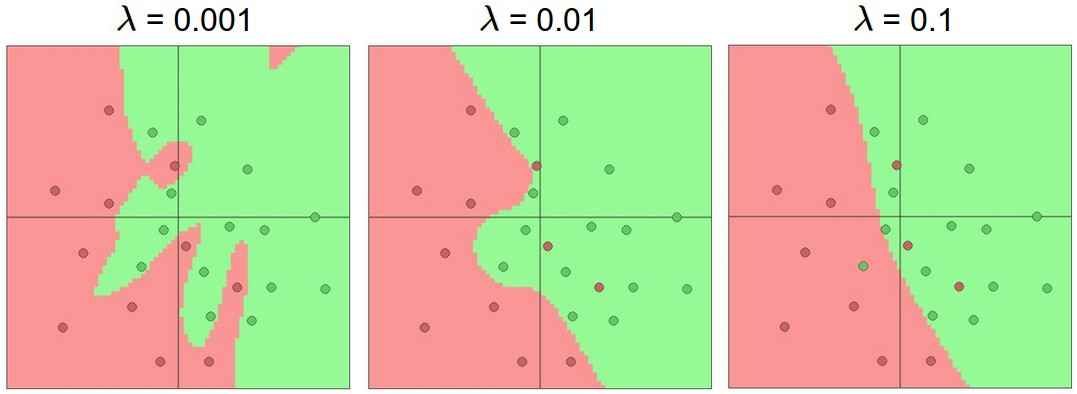
\includegraphics[width=1\linewidth]{figures/comparacao_regularizacao}
		\end{figure}
	Vamos implementar no notebook de redes neurais os métodos de regularização vistos
	\end{block}

\end{frame}
%==========================================================================================
\begin{frame}
	\frametitle{Técnica Momentum}
	\begin{block}{Momentum}
		\begin{itemize}
			\item Utilizada no gradiente descendente
			\item Adiciona velocidade ao Gradiente Descendente
			\item Soma o gradiente da iteração anterior $t-1$ multiplicado por um fator momentum $\mu$
			\item 	\href{https://github.com/mafaldasalomao/pavic_treinamento_ml/blob/main/Machine_Learning/figures/nomomentum1d.gif?raw=true}{\beamergotobutton{Sem Momentum}}
			\item \href{https://github.com/mafaldasalomao/pavic_treinamento_ml/blob/main/Machine_Learning/figures/momentum1d.gif?raw=true}{\beamergotobutton{Com Momentum}}
			\item Fonte \href{https://machinelearningcoban.com/2017/01/16/gradientdescent2/}{\beamergotobutton{Fonte}}
			
		\end{itemize}
		
		$$\triangledown w = \eta \frac{\partial J}{\partial w} + \mu \triangledown w^{t-1}$$
		Vamos implementar no notebook de redes neurais o nosso momentum
	\end{block}
\end{frame}
%==========================================================================================


%==========================================================================================
\begin{frame}
	\frametitle{Mini-Batch}
	\begin{block}{Mini-Batch}
		\begin{itemize}
			\item Divide o treinamento em conjuntos menores (memória)
			\item É importante dar shuffle (embaralhar) antes de cada epoch
			\item 1 epoch = processar todos os batchs
			\item Em geral, é a estratégia de GD mais utilizada	
			
		\end{itemize}
		Vamos tomar um dataset com $100$ amostras e seja dividi-lo em $10$ batchs. Cada batch terá $10$ amostras.
		\begin{figure}
			\centering
			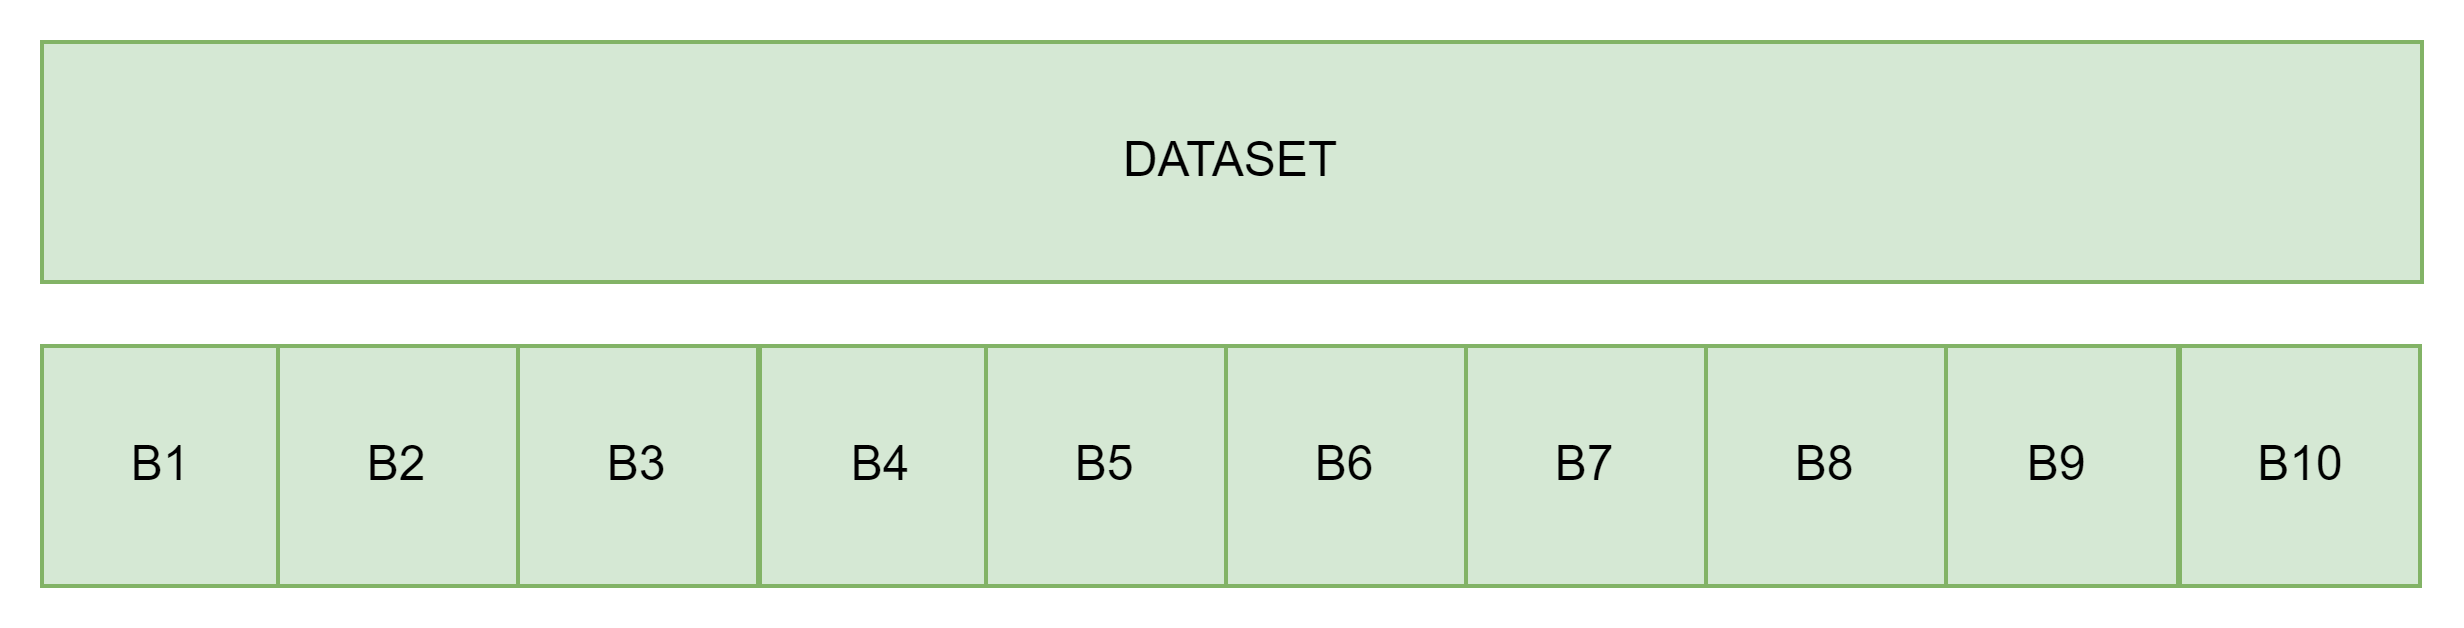
\includegraphics[width=1\linewidth]{figures/minibatch.png}
		\end{figure}
		
	\end{block}
\end{frame}
%==========================================================================================
\begin{frame}
	\frametitle{Gradiente Descendente}
	\begin{block}{Gradiente Descendente}
		Qual a diferença entre o Gradiente Estocástico para o Gradiente Baseado em Mini-batch e Bath \\
		\begin{columns}
			\begin{column}{0.3 \textwidth}
				\textbf{Stochastic Gradient} \\
				Amostra por amostra\\
				Aponta para a direção da amostra \\
				Converge lentamente \\
				Anula vetorização
			\end{column}
			\begin{column}{0.3 \textwidth}
				\textbf{Mini-Batch GD} \\
				Calcula as atualizações por lote \\
				Aponta para a direção que desce \\
				Converge rápido \\
				Rápida execução
			\end{column}
			\begin{column}{0.3 \textwidth}
				\textbf{Batch GD} \\
				Todas as amostras de uma vez \\
				Aponta para a direção que desce sempre \\
				Converge rápido \\
				Lenta execução
			\end{column}
		\end{columns}
		
	\end{block}
\end{frame}

	
%==========================================================================================
\begin{frame}
	\frametitle{Learning Rate Decay}
	\begin{block}{Learning Rate Decay}
		\begin{itemize}
			\item A learning rate alta irá dificultar o aprendizado do algoritmo, mas se livrará de mínimos locais
			\item A learning rate baixa irá ajudar no aprendizado da rede mas irá ter problemas com mínimos locais
			\item Com a Learning Rate Decay, a taxa de aprendizado será reduzida ao longo das épocas
		\end{itemize}
	\end{block}
\end{frame}	
	%==========================================================================================
	\begin{frame}
		\frametitle{Learning Rate Decay}
		\begin{block}{Learning Rate Decay - Time-based}
			$$\lambda_t = \frac{1}{1 + \alpha *t}$$ 
			Onde $t$ são as épocas
			\begin{columns}
				\begin{column}{0.3 \textwidth}
					\begin{figure}
						\centering
						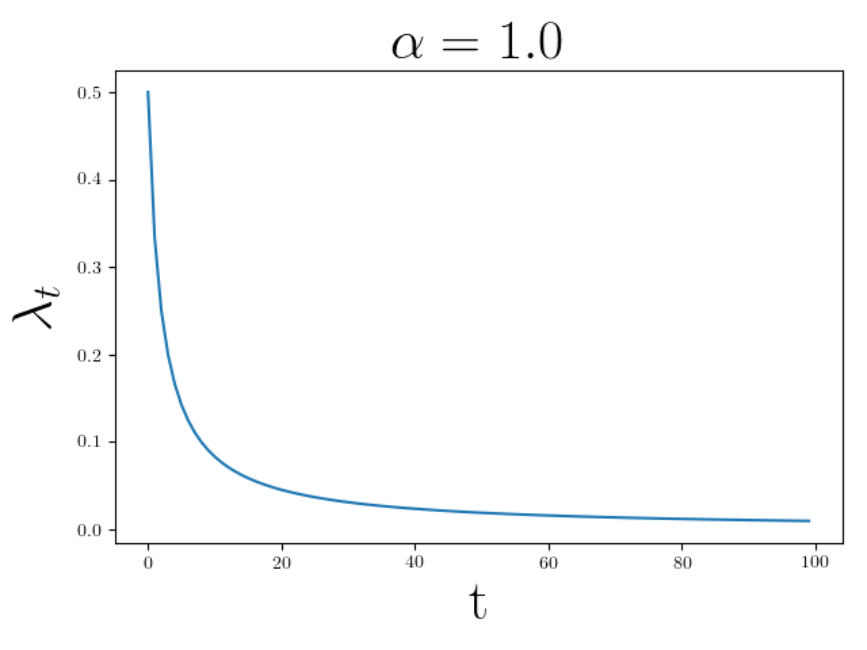
\includegraphics[width=1\linewidth]{figures/lr_decay1.png}
					\end{figure}
				\end{column}
				\begin{column}{0.3 \textwidth}
					\begin{figure}
						\centering
						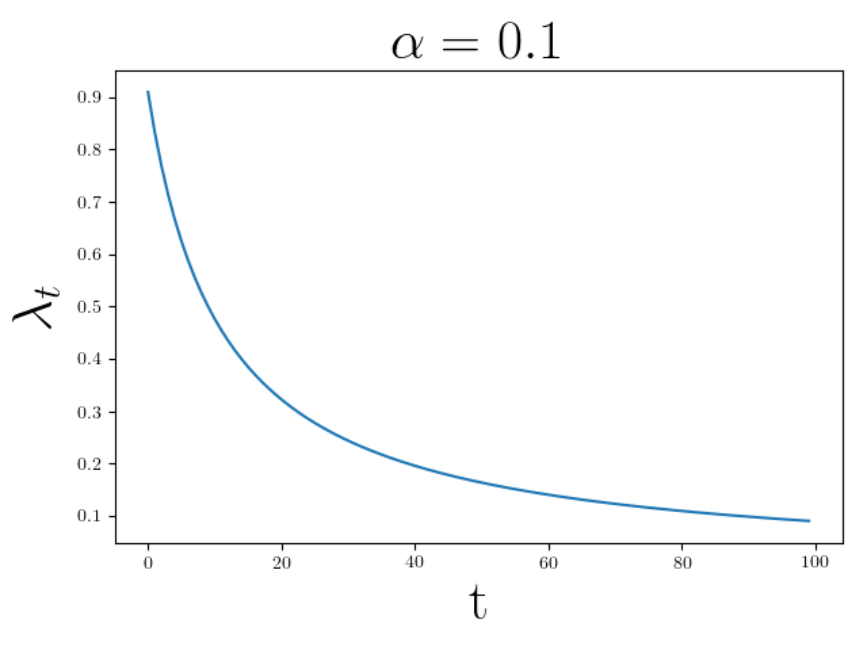
\includegraphics[width=1\linewidth]{figures/lr_decay2.png}
					\end{figure}
				\end{column}
				\begin{column}{0.3 \textwidth}
					\begin{figure}
						\centering
						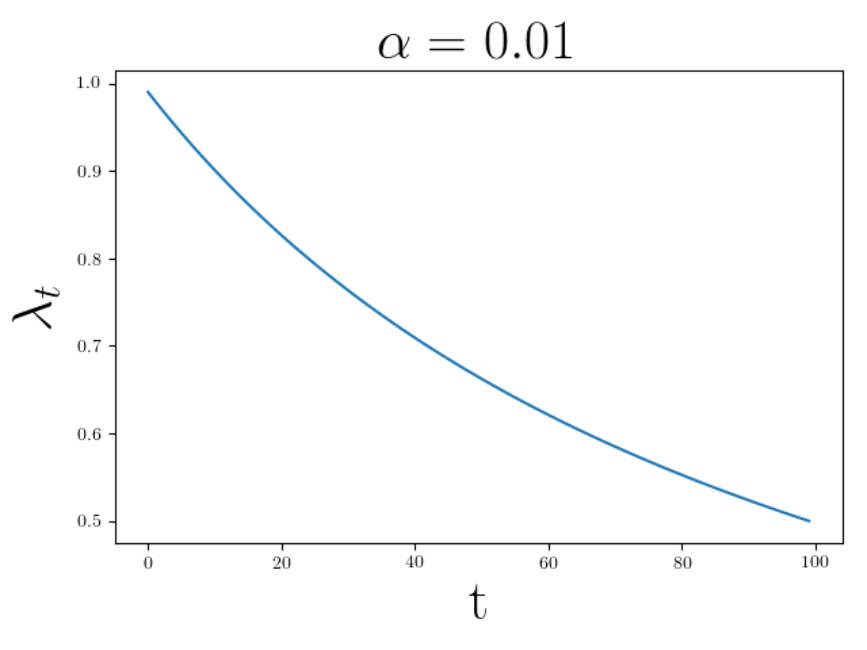
\includegraphics[width=1\linewidth]{figures/lr_decay3.png}
					\end{figure}
				\end{column}
			\end{columns}
		\end{block}
	\end{frame}	

%==========================================================================================
\begin{frame}
	\frametitle{Learning Rate Decay}
	\begin{block}{Learning Rate Decay - Exponential}
		$$\lambda_t = \lambda_0 *\alpha^t$$ 
		Onde $\alpha^t$ é o fator exponencial do decaimento da Learning rate
		\begin{columns}
			\begin{column}{0.3 \textwidth}
				\begin{figure}
					\centering
					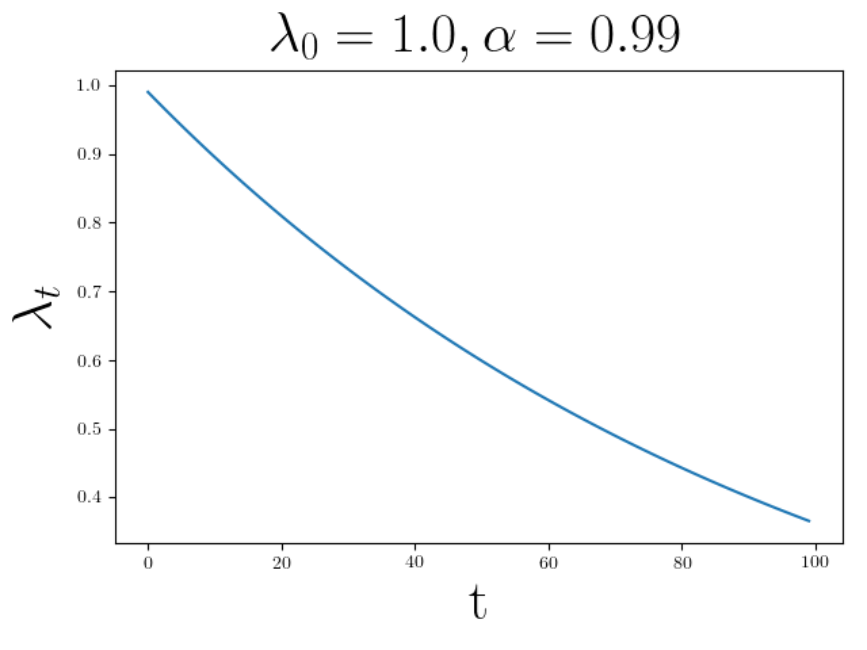
\includegraphics[width=1\linewidth]{figures/lr_decay4.png}
				\end{figure}
			\end{column}
			\begin{column}{0.3 \textwidth}
				\begin{figure}
					\centering
					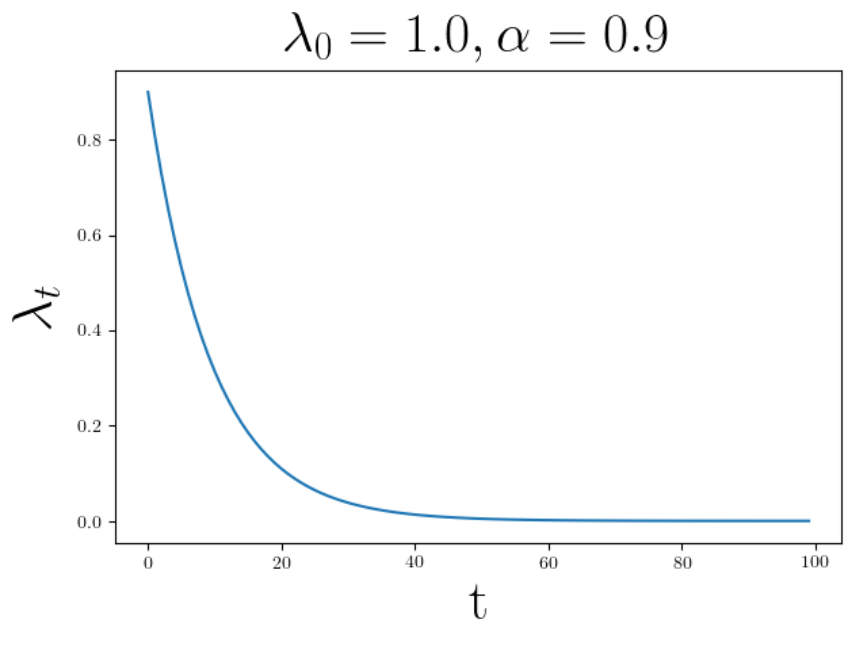
\includegraphics[width=1\linewidth]{figures/lr_decay5.png}
				\end{figure}
			\end{column}
			\begin{column}{0.3 \textwidth}
				\begin{figure}
					\centering
					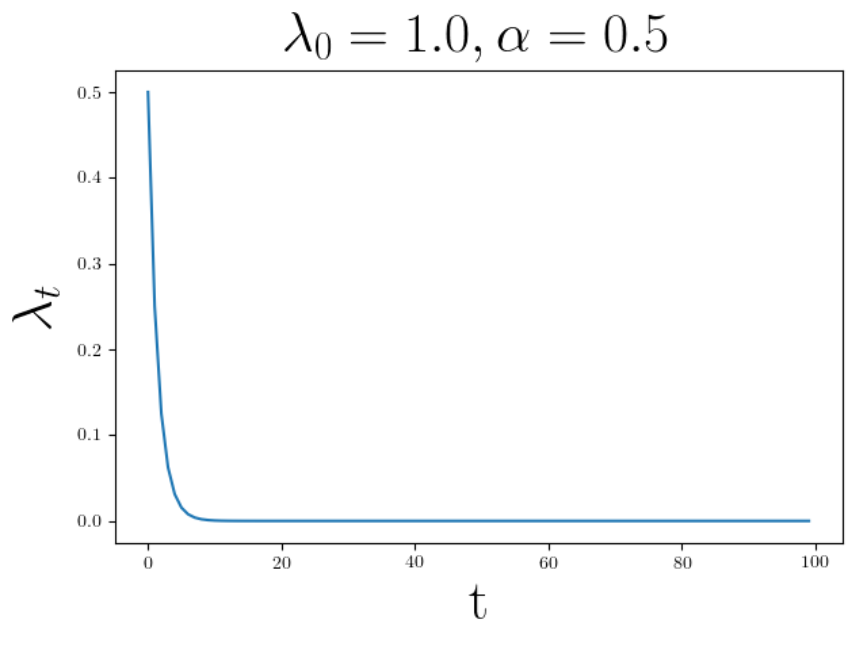
\includegraphics[width=1\linewidth]{figures/lr_decay6.png}
				\end{figure}
			\end{column}
		\end{columns}
	\end{block}
\end{frame}	
%==========================================================================================
\begin{frame}
		\frametitle{Learning Rate Decay}
		\begin{block}{Learning Rate Decay - Staircase}
			$$\lambda_t = \lambda_0 *\alpha^{t/ds}$$ 
			Onde $\alpha^{t/ds}$ é o fator exponencial do decaimento da Learning rate e o $ds$ é de quanta em quanta épocas ocorrerá o decay.
			\begin{columns}
				\begin{column}{0.3 \textwidth}
					\begin{figure}
						\centering
						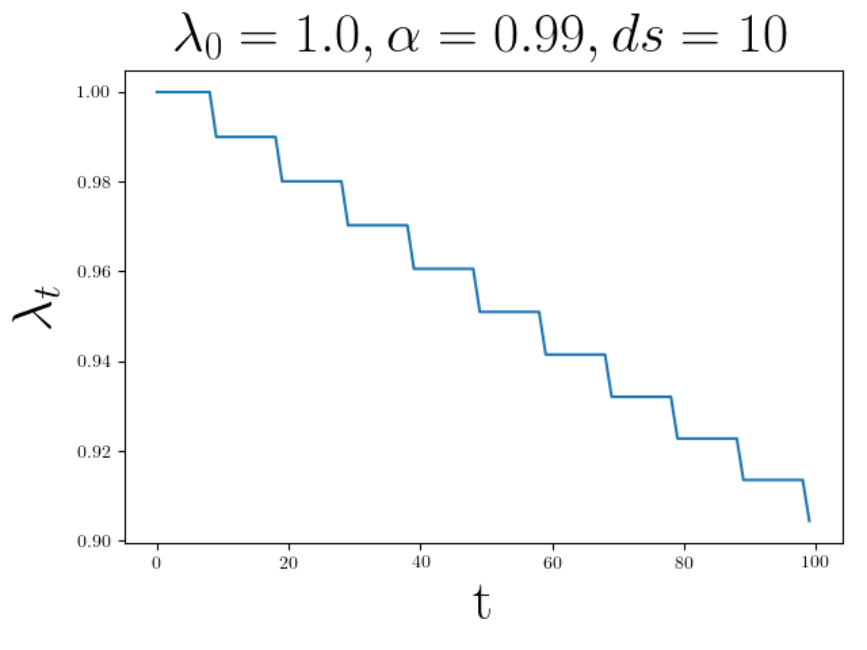
\includegraphics[width=1\linewidth]{figures/lr_decay7.png}
					\end{figure}
				\end{column}
				\begin{column}{0.3 \textwidth}
					\begin{figure}
						\centering
						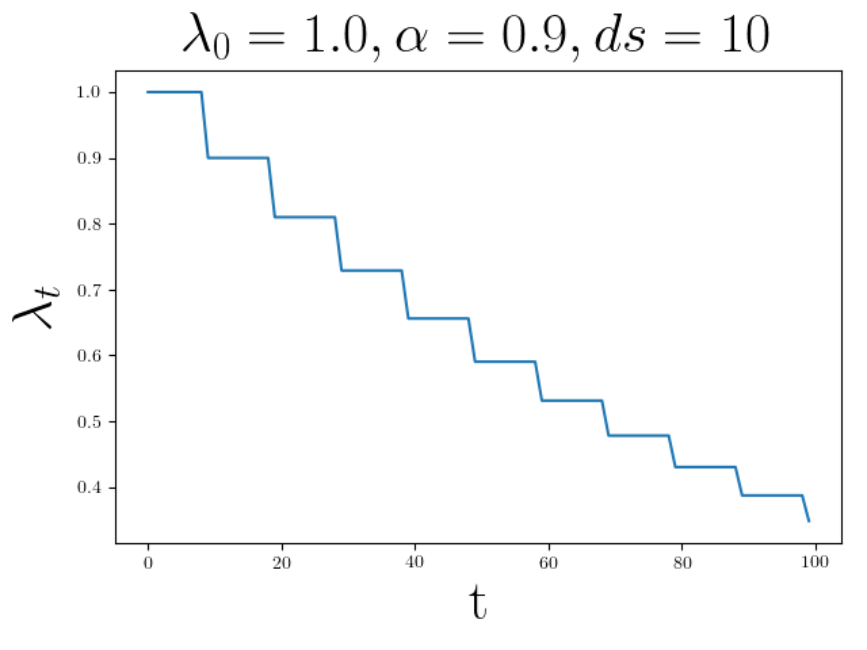
\includegraphics[width=1\linewidth]{figures/lr_decay8.png}
					\end{figure}
				\end{column}
				\begin{column}{0.3 \textwidth}
					\begin{figure}
						\centering
						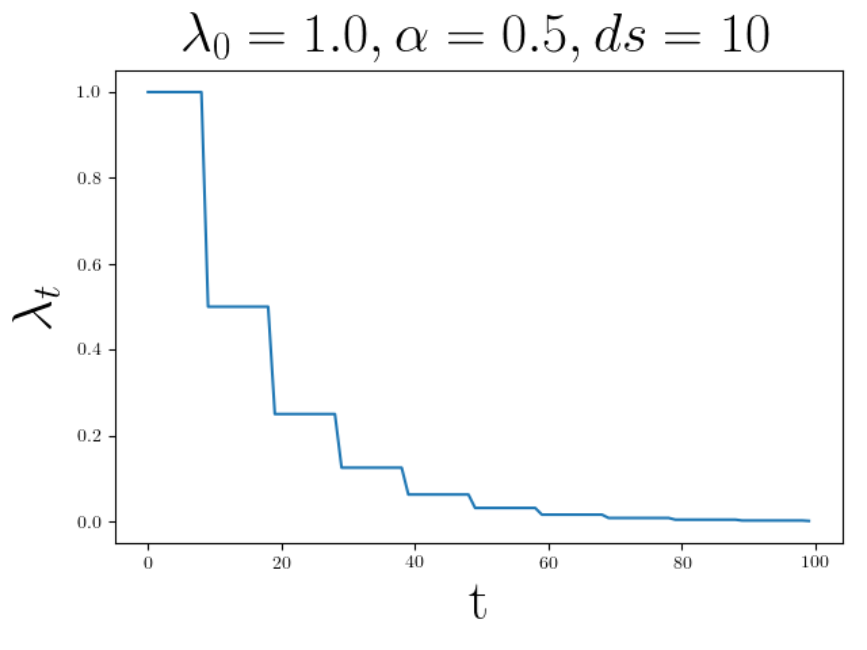
\includegraphics[width=1\linewidth]{figures/lr_decay9.png}
					\end{figure}
				\end{column}
			\end{columns}
		\end{block}
	\end{frame}	
	
%==========================================================================================
\begin{frame}
	\frametitle{Stop Early}
	\begin{block}{Stop Early}
		\begin{itemize}
			\item A ideia é guardar seu melhor modelo. Quando a perda tiver valor mínimo em validação!
			\item Fator patient indica quando o modelo deve parar de treinar a partir da última melhor acurácia. Por exemplo, se na época 7 o modelo apresentou acurácia de 75\% e nas 10 (patient) próximas épocas o modelo não melhorou, então o treinamento é finalizado.
		\end{itemize}
		\begin{figure}
			\centering
			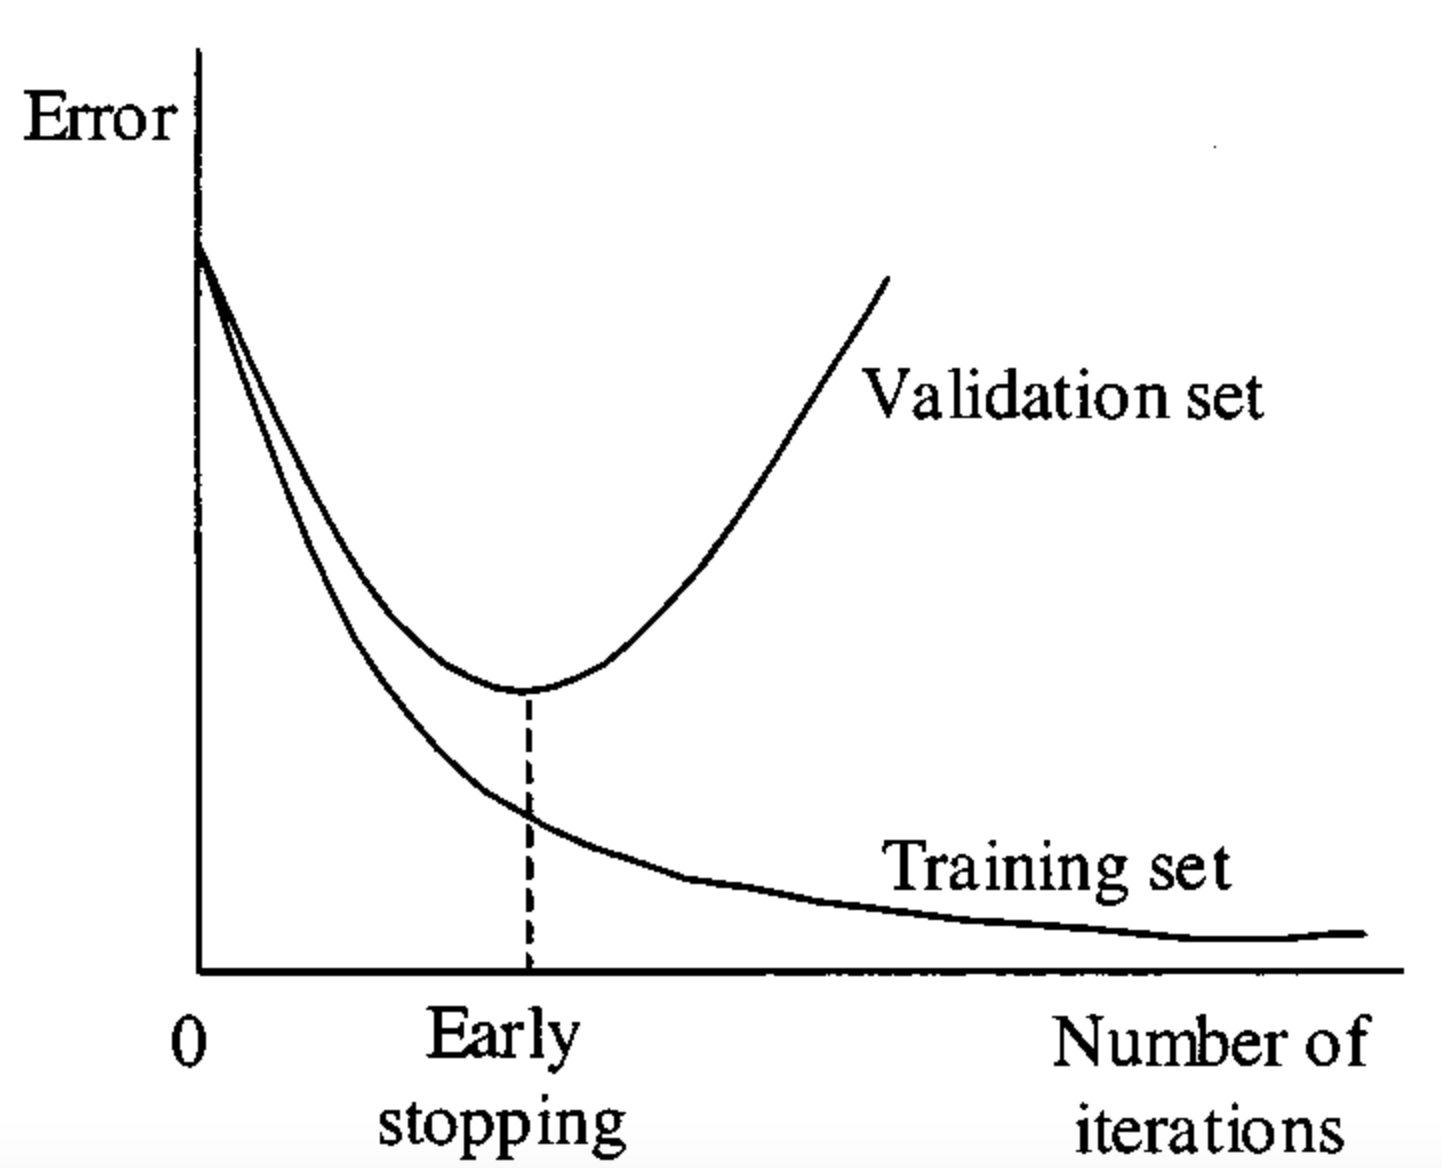
\includegraphics[width=0.35\linewidth]{figures/early_stop}
		\end{figure}
	\end{block}
\end{frame}	
	
%==========================================================================================
\begin{frame}
	\frametitle{Batch Normalization}
	\begin{block}{Batch Normalization}
		\begin{itemize}
			\item Normaliza entradas ou saídas das camadas de ativação
			\item Estima a média e desvio padrão baseado no batch (média móvel)
			\item Regulariza camadas e não neurônios
			\item Pode substituir o dropout
			\item Uma das melhores técnicas
			\item Não usado na validação ou teste!
		\end{itemize}
	\end{block}
\end{frame}	

%==========================================================================================
\begin{frame}
	\frametitle{Batch Normalization}
	\begin{block}{Batch Normalization - FeedForward}
	\begin{columns}
		\begin{column}{0.5 \textwidth}
			\begin{figure}
				\centering
				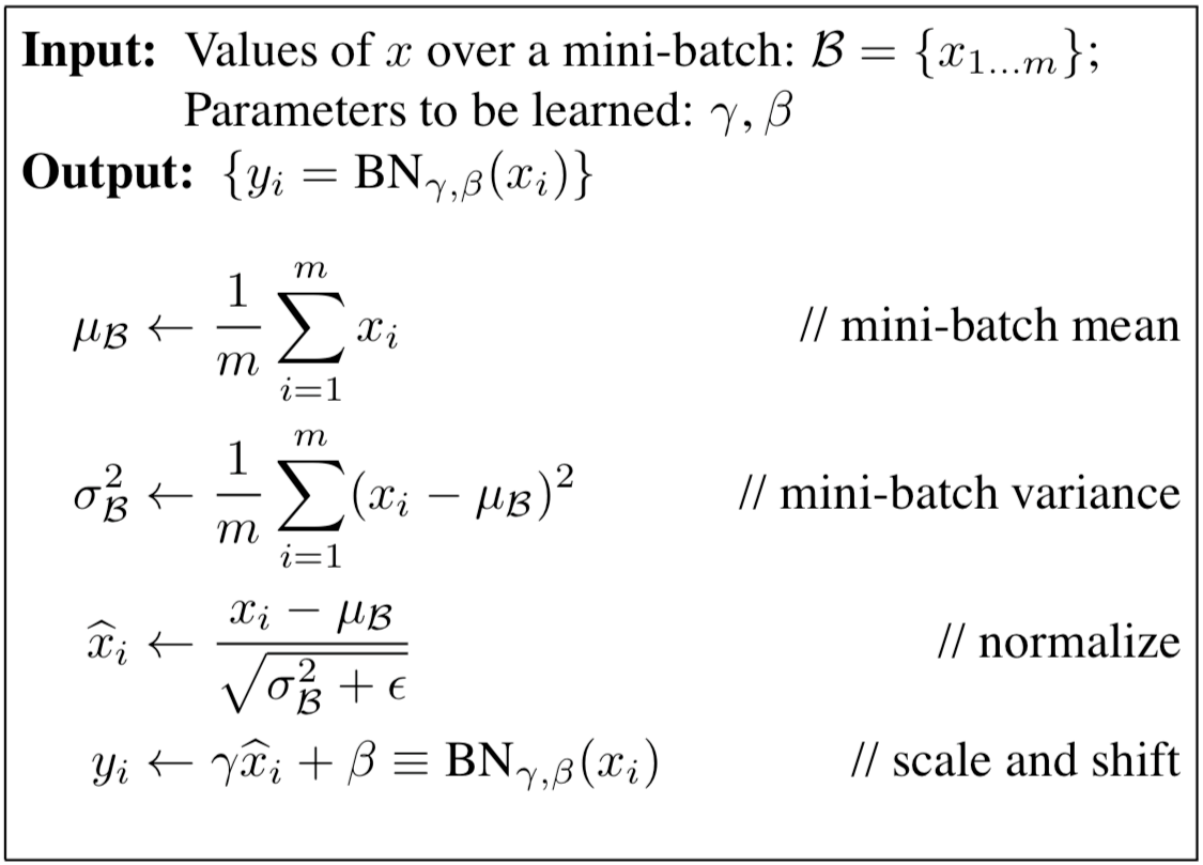
\includegraphics[width=1\linewidth]{figures/batch_norm_feed.png}
			\end{figure}
		\end{column}
		\begin{column}{0.5 \textwidth}
			\begin{itemize}
				\item Cada batch será normalizado subtraindo da média $\mu$ e dividindo pelo desvio padrão $\sigma^2$ = $\hat{x}_i$
				\item $\gamma$ e $\beta$ são parâmetros que a rede vai aprender
				\item se $\gamma = \sigma^2 $ e $\mu = \beta$ a função se anula, assim a rede pode recusar o batch normalization sozinha!
			\end{itemize}
		\end{column}
	\end{columns}

	\end{block}
\end{frame}	
	
%==========================================================================================
\begin{frame}
	\frametitle{Batch Normalization}
	\begin{block}{Batch Normalization - Backpropagation}
		\begin{figure}
			\centering
			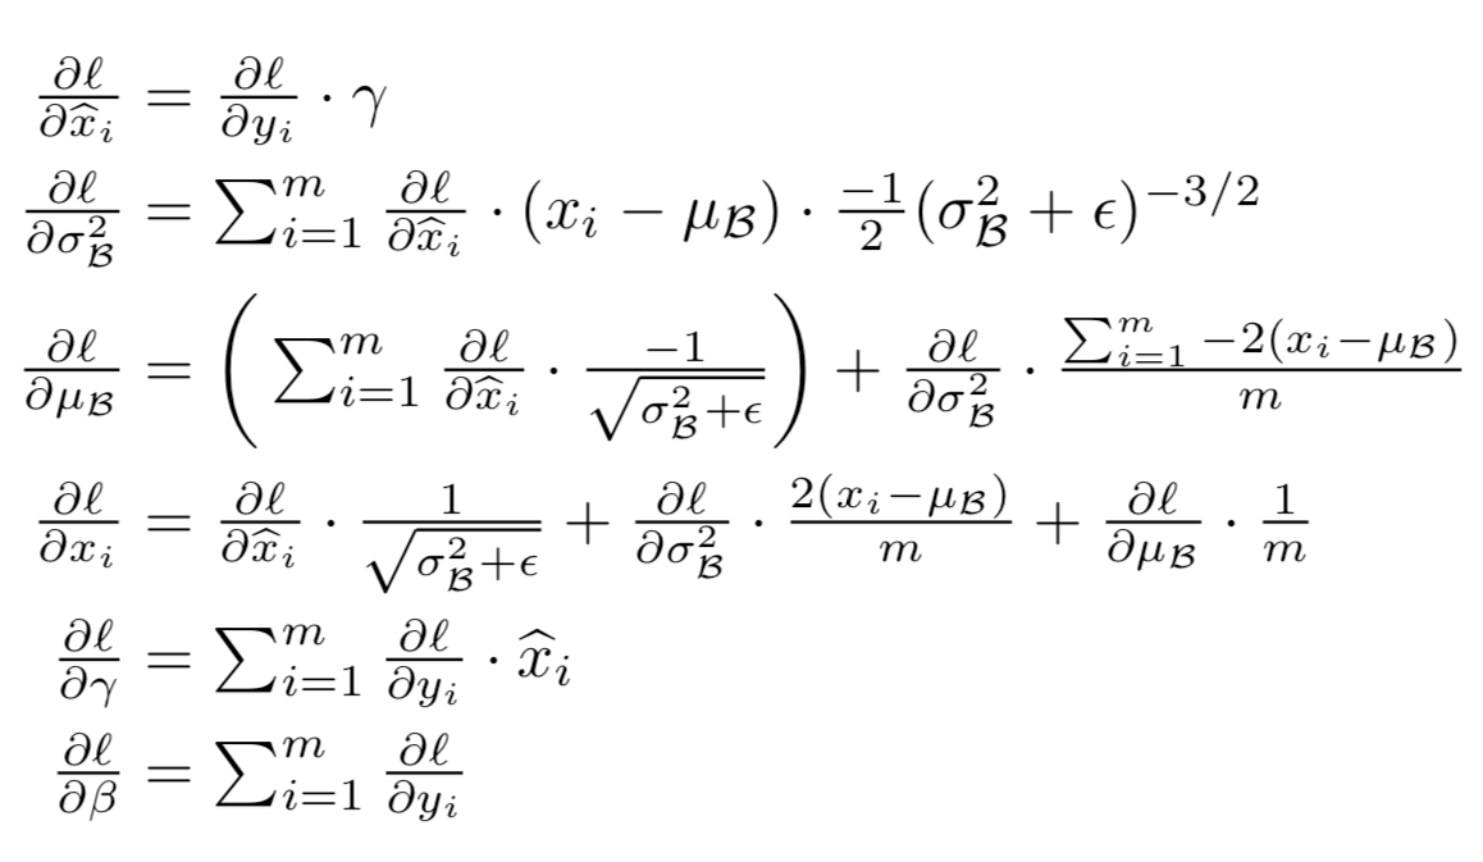
\includegraphics[width=1\linewidth]{figures/batch_norm_back.png}
		\end{figure}
	\end{block}
\end{frame}		
	
%==========================================================================================
\begin{frame}
	\frametitle{Freezing}
	\begin{block}{Freezing}
		\begin{itemize}
			\item Congelamento de certas camadas no \textbf{treinamento}
			\item Muito usada em transfer learning e Fine-tuning
		\end{itemize}
		\begin{figure}
			\centering
			\includegraphics[width=0.7\linewidth]{figures/simple_nn.png}
		\end{figure}
	\end{block}
\end{frame}			
	
	
	
	
\begin{frame}	
\frametitle{Highlighting text}
%
%\begin{align}
%	a + b  q q= c \\        
%	a = c - b
%\end{align}
In this slide, some important text will be
\alert{highlighted} because it's important.
Please, don't abuse it.

\begin{block}{Remark}
Sample text
\end{block}

\begin{alertblock}{Important theorem}
Sample text in red box
\end{alertblock}

\begin{examples}
Sample text in green box. The title of the block is ``Examples".
\end{examples}
\end{frame}

\end{document}